%%%%%%%%%%%%%%%%%%%%%%%%%%%%%%%%%%%%%%%%%%%%%%%%%%%%%%%%%%%%%%%%%%
%%%%%%%%%%%%%%%%%%%%%%%%%%%%%%%%%%%%%%%%%%%%%%%%%%%%%%%%%%%%%%%%%%
\chapter{Multivariate Verfahren}
\label{sec:multivariate}
%%%%%%%%%%%%%%%%%%%%%%%%%%%%%%%%%%%%%%%%%%%%%%%%%%%%%%%%%%%%%%%%%%
%%%%%%%%%%%%%%%%%%%%%%%%%%%%%%%%%%%%%%%%%%%%%%%%%%%%%%%%%%%%%%%%%%

\index{multivariate Verfahren}
Liegen von Beobachtungsobjekten Werte mehrerer Variablen vor, kann sich die Datenanalyse nicht nur auf jede Variable einzeln, sondern auch auf die gemeinsame Verteilung der Variablen beziehen. Solche Fragestellungen sind mit multivariaten Verfahren zu bearbeiten \cite{Backhaus2008, Backhaus2013}, deren Anwendung in R \citeA{Zelterman2015} vertiefend behandelt. Abschnitte \ref{sec:distr2var}, \ref{sec:3dPlot} und \ref{sec:ggplotFacet} thematisieren Möglichkeiten, multivariate Daten in Diagrammen zu veranschaulichen.

%%%%%%%%%%%%%%%%%%%%%%%%%%%%%%%%%%%%%%%%%%%%%%%%%%%%%%%%%%%%%%%%%%
%%%%%%%%%%%%%%%%%%%%%%%%%%%%%%%%%%%%%%%%%%%%%%%%%%%%%%%%%%%%%%%%%%
\section{Lineare Algebra}
\label{sec:linAlg}
%%%%%%%%%%%%%%%%%%%%%%%%%%%%%%%%%%%%%%%%%%%%%%%%%%%%%%%%%%%%%%%%%%
%%%%%%%%%%%%%%%%%%%%%%%%%%%%%%%%%%%%%%%%%%%%%%%%%%%%%%%%%%%%%%%%%%

\index{lineare Algebra|see{Matrix}}
Vielen statistischen Auswertungen -- insbesondere im Bereich multivariater Verfahren -- liegt im Kern das Rechnen mit Matrizen zugrunde. Deshalb soll an dieser Stelle auf einige grundlegende Funktionen zur Matrix-Algebra eingegangen werden, Details beschreibt \citeA{Fieller2017}. Die gezeigten Zusammenhänge sind nur für manuelle Kontrollrechnungen relevant, nicht aber für die reine Anwendung multivariater Tests mit R-eigenen Funktionen.\footnote{Die hier vorgestellten Rechenwege setzen die mathematischen Formeln direkt um. Tatsächlich gibt es häufig numerisch effizientere und stabilere Möglichkeiten, um dieselben Ergebnisse zu erhalten. So entspricht die Implementierung von R-eigenen Funktionen auch meist nicht den hier vorgestellten Rechnungen \cite{Bates2004}. Abschnitt \ref{sec:performance} erläutert Wege, die Effizienz der Berechnungen zu steigern. Das Paket\index[pack]{Matrix@\lstinline{Matrix}} \lstinline!Matrix! \cite{Bates2009} enthält fortgeschrittene Methoden der Matrix-Algebra -- etwa zu schwachbesetzten Matrizen, die u.\,a.\ als Designmatrizen linearer Modelle auftauchen (Abschn.\ \ref{sec:multALMregr}).} Die Rechentechniken und zugehörigen Konzepte der linearen Algebra seien als bekannt vorausgesetzt \cite{Fischer2008, Strang2003}.

%%%%%%%%%%%%%%%%%%%%%%%%%%%%%%%%%%%%%%%%%%%%%%%%%%%%%%%%%%%%%%%%%%
%%%%%%%%%%%%%%%%%%%%%%%%%%%%%%%%%%%%%%%%%%%%%%%%%%%%%%%%%%%%%%%%%%
\subsection{Matrix-Algebra}
\label{sec:matAlg}
%%%%%%%%%%%%%%%%%%%%%%%%%%%%%%%%%%%%%%%%%%%%%%%%%%%%%%%%%%%%%%%%%%
%%%%%%%%%%%%%%%%%%%%%%%%%%%%%%%%%%%%%%%%%%%%%%%%%%%%%%%%%%%%%%%%%%

\index[func]{t()@\lstinline{t()}}
\index{Matrix!transponieren}
\index{transponieren|see{Matrix}}
Eine Matrix $\bm{X}$ wird mit \lstinline!t(X)! transponiert. Hierdurch werden die Zeilen von $\bm{X}$ zu den Spalten der Transponierten $\bm{X}^{\top}$ und die Spalten von $\bm{X}$ zu Zeilen von $\bm{X}^{\top}$. Es gilt $(\bm{X}^{\top})^{\top} = \bm{X}$.
\begin{lstlisting}
> N  <- 4                             # Anzahl Zeilen
> p  <- 2                             # Anzahl Spalten
> (X <- matrix(c(20, 26, 10, 19, 29, 27, 20, 12), nrow=N, ncol=p))
     [,1]  [,2]
[1,]   20    29
[2,]   26    27
[3,]   10    20
[4,]   19    12

> t(X)                                # Transponierte
     [,1]  [,2]  [,3]  [,4]
[1,]   20    26    10    19
[2,]   29    27    20    12
\end{lstlisting}

\index[func]{diag()@\lstinline{diag()}}
\index{Matrix!Diagonalmatrix}
\index{Matrix!Einheitsmatrix}
\lstinline!diag(<<Vektor>>)! erzeugt eine Diagonalmatrix, deren Diagonale aus den Elementen von \lstinline!<<Vektor>>! besteht. Besitzt der übergebene Vektor allerdings nur ein Element, liefert die Variante \lstinline!diag(<<Anzahl>>)! als besondere Diagonalmatrix eine Einheitsmatrix mit \lstinline!<<Anzahl>>! vielen Zeilen und Spalten.\footnote{Eine Dezimalzahl wird dabei tranchiert. Eine $(1 \times 1)$-Diagonalmatrix $\bm{X}$ kann mit einem weiteren Argument als \lstinline!diag(x, nrow=1)! erzeugt werden.}
\begin{lstlisting}
# Diagonale der Kovarianzmatrix von X -> Varianzen der Spalten von X
> diag(cov(X))
[1] 43.58333 59.33333

> diag(1:3)                       # Diagonalmatrix mit Diagonale 1,2,3
     [,1]  [,2]  [,3]
[1,]    1     0     0
[2,]    0     2     0
[3,]    0     0     3

> diag(2)                         # 2x2 Einheitsmatrix
     [,1]  [,2]
[1,]    1     0
[2,]    0     1
\end{lstlisting}

\index{Matrix!Algebra}
\index{Matrix!Multiplikation}
\index{Matrix!Skalarprodukt}
\index{Matrix!Addition}
\index{Matrix!Kronecker-Produkt}
\index{Matrix!Hadamard-Produkt}
\index{Skalarprodukt|see{Matrix}}
\index{Vektor!Skalarprodukt|see{Matrix}}
\index{Vektor!Kreuzprodukt}
\index[func]{\%^\%@\texttt{\%\^{}\%}}
\index[func]{\%*\%@\texttt{\%*\%}}
Da auch bei Matrizen die herkömmlichen Operatoren elementweise arbeiten, eignet sich für die Addition von Matrizen $\bm{X}$ und $\bm{Y}$ gleicher Dimensionierung der \lstinline!+! Operator mit \lstinline!X + Y! genauso wie \lstinline!*! für die Multiplikation von Matrizen mit einem Skalar mittels \lstinline!<<Matrix>> * <<Zahl>>!. Auch \lstinline!X * Y! ist als elementweises Hadamard-Produkt $\bm{X} \circ \bm{Y}$ von gleich dimensionierten Matrizen zu verstehen. Die Matrix-Multiplikation einer $(p \times q)$-Matrix $\bm{X}$ mit einer $(q \times r)$-Matrix $\bm{Y}$ lässt sich dagegen mit \lstinline!X %*% Y! formulieren.\footnote{Mit dem Operator \lstinline!<<Matrix>> \%^\% <<Zahl>>! aus dem Paket\index[pack]{expm@\lstinline{expm}|textbf} \lstinline!expm! \cite{Goulet2010} ist das Exponenzieren von quadratischen Matrizen möglich, mit\index[func]{logm()@\lstinline{logm()}} \lstinline!logm()! aus demselben Paket das Logarithmieren.} Das Ergebnis ist die $(p \times r)$-Matrix der Skalarprodukte der Zeilen von $\bm{X}$ mit den Spalten von $\bm{Y}$. Als Rechenregel ist in vielen Situationen $(\bm{X} \bm{Y})^{\top} = \bm{Y}^{\top} \bm{X}^{\top}$ relevant.

Für den häufig genutzten Spezialfall $\bm{X}^{\top} \bm{Y}$ existiert die Funktion\index[func]{crossprod()@\lstinline{crossprod()}} \lstinline!crossprod(X, Y)!, die alle paarweisen Skalarprodukte der Spalten von $\bm{X}$ und $\bm{Y}$ berechnet.\footnote{Sie ist zudem numerisch effizienter als die Verwendung von \lstinline!t(X) \%*\% Y!. Die Benennung erscheint unglücklich, da Verwechslungen mit dem Vektor-Kreuzprodukt naheliegen, das man stattdessen mit\index[func]{cross()@\lstinline{cross()}} \lstinline!cross()! aus dem Paket\index[pack]{pracma@\lstinline{pracma}} \lstinline!pracma! \cite{Borchers2011} erhält.} \lstinline!crossprod(X)! ist die Kurzform für $\bm{X}^{\top} \bm{X}$. Das Kronecker-Produkt $\bm{X} \otimes \bm{Y}$ erhält man mit der Funktion\index[func]{kronecker()@\lstinline{kronecker()}} \lstinline!kronecker()!, deren Operator-Schreibweise\index[func]{\%x\%@\texttt{\%x\%}} \lstinline!X %x% Y! lautet.

Die Matrix-Multiplikation ist auch auf Vektoren anwendbar, da diese als Matrizen mit nur einer Zeile bzw.\ einer Spalte aufgefasst werden können. Mit \lstinline!c()! oder \lstinline!numeric()! erstellte Vektoren werden in den meisten Rechnungen automatisch so in Zeilen- oder Spaltenvektoren konvertiert, dass die Rechenregeln erfüllt sind.
\begin{lstlisting}
# c(1, 2) wie Zeilenvektor behandelt: (1x2) Vektor %*% (2x3) Matrix
> c(1, 2) %*% rbind(c(1, 2, 3), c(4, 5, 6))
     [,1] [,2] [,3]
[1,]    9   12   15

# c(7, 8, 9) wie Spaltenvektor behandelt: (2x3) Matrix %*% (3x1) Vektor
> rbind(c(1, 2, 3), c(4, 5, 6)) %*% c(7, 8, 9)
     [,1]
[1,]   50
[2,]  122
\end{lstlisting}

Das Skalarprodukt zweier Vektoren $\bm{x}$ und $\bm{y}$ ist mit \lstinline!crossprod(x, y)! oder mit \lstinline!sum(x*y)! berechenbar. Das Ergebnis von \lstinline!crossprod()! ist dabei immer eine Matrix, auch wenn diese nur aus einer Spalte oder einzelnen Zahl besteht.

Als Beispiel sollen einige wichtige Matrizen zu einer gegebenen $(n \times p)$-Datenmatrix $\bm{X}$ mit Variablen in den Spalten berechnet werden: Die spaltenweise zentrierte Datenmatrix $\dot{\bm{X}}$ führt zur\index{Matrix!SSP-Matrix} SSP-Matrix $\dot{\bm{X}}^{\top} \dot{\bm{X}}$ (auch SSCP-Matrix genannt, \emph{sum of squares and cross products}).\footnote{\index{Matrix!zentrieren}Im Anwendungsfall sollte man statt einer Zentriermatrix die Funktion \lstinline!scale(<<Matrix>>, center=TRUE, scale=FALSE)! verwenden, um eine Matrix spaltenweise zu zentrieren.} Sie ist das $(n-1)$-fache der korrigierten Kovarianzmatrix $\bm{S}$.
\begin{lstlisting}
> (Xc <- diag(N) - matrix(rep(1/N, N^2), nrow=N))     # Zentriermatrix
      [,1]   [,2]   [,3]   [,4]
[1,]  0.75  -0.25  -0.25  -0.25
[2,] -0.25   0.75  -0.25  -0.25
[3,] -0.25  -0.25   0.75  -0.25
[4,] -0.25  -0.25  -0.25   0.75

> all.equal(Xc %*% Xc, Xc)            # Zentriermatrix ist idempotent
[1] TRUE

> (Xdot <- Xc %*% X)                  # spaltenweise zentrierte Daten
      [,1]  [,2]
[1,]  1.25     7
[2,]  7.25     5
[3,] -8.75    -2
[4,]  0.25   -10

> (SSP <- t(Xdot) %*% Xdot)           # SSP-Matrix
       [,1]  [,2]
[1,] 130.75    60
[2,]  60.00   178

> crossprod(Xdot)                     # äquivalent: SSP-Matrix ...
> (1/(N-1)) * SSP                     # korrigierte Kovarianzmatrix
         [,1]      [,2]
[1,] 43.58333  20.00000
[2,] 20.00000  59.33333

> (S <- cov(X))                       # korrigierte Kovarianzmatrix
         [,1]      [,2]
[1,] 43.58333  20.00000
[2,] 20.00000  59.33333
\end{lstlisting}

Mit Hilfe der aus den Kehrwerten der korrigierten Streuungen gebildeten Diagonalmatrix $\bm{D}_{S}^{-1/2}$ erhält man die zu einer Kovarianzmarix $\bm{S}$ gehörende Korrelationsmatrix als $\bm{R} = \bm{D}_{S}^{-1/2} \bm{S} \bm{D}_{S}^{-1/2}$. Hierfür eignet sich\index[func]{cov2cor()@\lstinline{cov2cor()}} \lstinline!cov2cor(<<K>>)!.
\begin{lstlisting}
> Dsi <- diag(1/sqrt(diag(S)))        # Diagonalmatrix: 1 / Streuungen
> Dsi %*% S %*% Dsi                   # Korrelationsmatrix
          [,1]       [,2]
[1,] 1.0000000  0.3932968
[2,] 0.3932968  1.0000000

> cov2cor(S)                          # Kontrolle ...
\end{lstlisting}

Für Anwendungen, in denen die Zeilen oder Spalten einer Matrix $\bm{X}$ mit einem Vektor $\bm{a}$ verrechnet werden müssen, eignet sich \lstinline!sweep()! (Abschn.\ \ref{sec:mat_colwise}). So könnte $\bm{a}$ etwa zu jeder Zeile von $\bm{X}$ addiert oder $\bm{X}$ spaltenweise normiert werden. Alternativ könnte letzteres auch mit $\bm{X} \bm{D}$ geschehen, wenn $\bm{D}$ die Diagonalmatrix aus den Kehrwerten der Spaltenlängen ist.
\begin{lstlisting}
> b <- 2                              # Skalar
> a <- c(-2, 1)                       # Vektor
> sweep(b * X, 2, a, "+")             # bX + a
     [,1]  [,2]
[1,]   38    59
[2,]   50    55
[3,]   18    41
[4,]   36    25

> colLens <- sqrt(colSums(X^2))       # euklidische Längen der Spalten
> sweep(X, 2, colLens, "/")           # spaltenweise normierte Daten
          [,1]       [,2]
[1,] 0.5101443  0.6307329
[2,] 0.6631876  0.5872341
[3,] 0.2550722  0.4349882
[4,] 0.4846371  0.2609929

# äquivalent: Mult. mit Diag.-Matrix aus Kehrwerten der Spaltenlängen
> X %*% diag(1/colLens)               # ...
\end{lstlisting}

%%%%%%%%%%%%%%%%%%%%%%%%%%%%%%%%%%%%%%%%%%%%%%%%%%%%%%%%%%%%%%%%%%
%%%%%%%%%%%%%%%%%%%%%%%%%%%%%%%%%%%%%%%%%%%%%%%%%%%%%%%%%%%%%%%%%%
\subsection{Lineare Gleichungssysteme lösen}
\label{sec:matSolve}
%%%%%%%%%%%%%%%%%%%%%%%%%%%%%%%%%%%%%%%%%%%%%%%%%%%%%%%%%%%%%%%%%%
%%%%%%%%%%%%%%%%%%%%%%%%%%%%%%%%%%%%%%%%%%%%%%%%%%%%%%%%%%%%%%%%%%

\index{lineare Gleichungssysteme lösen}
\index{Matrix!Inverse}
Für die Berechnung der Inversen $\bm{A}^{-1}$ einer quadratischen Matrix $\bm{A}$ mit vollem Rang ist die Funktion \lstinline!solve(a=<<Matrix>>, b=<<Matrix>>)! zu nutzen, die die Lösung $\bm{x}$ des linearen Gleichungssystems $\bm{A} \bm{x} = \bm{b}$ liefert. Dabei ist für das Argument \lstinline!a! eine invertierbare quadratische Matrix und für \lstinline!b! ein Vektor oder eine Matrix passender Dimensionierung anzugeben. Fehlt das Argument \lstinline!b!, wird als rechte Seite des Gleichungssystems die passende Einheitsmatrix $\bm{I}$ angenommen, womit sich als Lösung für $\bm{x}$ in $\bm{A} \bm{x} = \bm{I}$ die Inverse $\bm{A}^{-1}$ ergibt.\footnote{Für die\index{Matrix!Pseudoinverse|textbf}\index{Pseudoinverse|see{Matrix}} Pseudoinverse\index[func]{ginv()@\lstinline{ginv()}} $\bm{A}^{+}$ einer nicht invertierbaren Matrix $\bm{A}$ vgl.\ \lstinline!ginv()!\index[func]{ginv()@\lstinline{ginv()}} aus dem\index[pack]{MASS@\lstinline{MASS}} \lstinline!MASS! Paket. Für solche Matrizen ermittelt \lstinline!Null()!\index[func]{Null()@\lstinline{Null()}} aus demselben Paket eine Basis des\index{Matrix!Kern}\index{Kern|see{Matrix}} Kerns von $\bm{A}^{\top}$ (\emph{null space}).}

Für $\bm{A}^{-1}$ gilt etwa $(\bm{A}^{-1})^{-1} = \bm{A}$, $(\bm{A}^{-1})^{\top} = (\bm{A}^{\top})^{-1}$ und $(\bm{A} \bm{B})^{-1} = \bm{B}^{-1} \bm{A}^{-1}$, wenn $\bm{B}$ ebenfalls eine invertierbare Matrix passender Dimensionierung ist.
\begin{lstlisting}
> Y <- matrix(c(1, 1, 1, -1), nrow=2)   # Matrix Y
> (Yinv <- solve(Y))                    # Inverse von Y
     [,1]  [,2]
[1,]  0.5   0.5
[2,]  0.5  -0.5

> Y %*% Yinv                            # Kontrolle: Einheitsmatrix
     [,1]  [,2]
[1,]    1     0
[2,]    0     1

# löse lineares Gleichungssystem
> A  <- matrix(c(9, 1, -5, 0), nrow=2)  # Matrix A
> b  <- c(5, -3)                        # Ergebnisvektor
> (x <- solve(A, b))                    # Lösung x von Ax = b
[1] -3.0 -6.4

> A %*% x                               # Kontrolle: reproduziere b
     [,1]
[1,]    5
[2,]   -3
\end{lstlisting}

%%%%%%%%%%%%%%%%%%%%%%%%%%%%%%%%%%%%%%%%%%%%%%%%%%%%%%%%%%%%%%%%%%
%%%%%%%%%%%%%%%%%%%%%%%%%%%%%%%%%%%%%%%%%%%%%%%%%%%%%%%%%%%%%%%%%%
\subsection{Norm und Abstand von Vektoren und Matrizen}
\label{sec:matNorm}
%%%%%%%%%%%%%%%%%%%%%%%%%%%%%%%%%%%%%%%%%%%%%%%%%%%%%%%%%%%%%%%%%%
%%%%%%%%%%%%%%%%%%%%%%%%%%%%%%%%%%%%%%%%%%%%%%%%%%%%%%%%%%%%%%%%%%

\index{Vektor!Norm}
\index{Matrix!Spaltennorm}
\index{Norm}
Das mit \lstinline!crossprod(<<Vektor>>)! ermittelte Skalarprodukt $\bm{x}^{\top} \bm{x}$ eines Vektors $\bm{x}$ mit sich selbst liefert ebenso wie \lstinline!sum(<<Vektor>>^2)! dessen quadrierte euklidische\index{Lange@Länge!Norm} Länge $\|\bm{x}\|^{2}$ als quadrierte Norm. Genauso eignen sich \lstinline!colSums(<<Matrix>>^2)! und \lstinline!crossprod(<<Matrix>>)!, um die quadrierten Spaltennormen einer Matrix zu ermitteln, die dort im Ergebnis in der Diagonale stehen.
\begin{lstlisting}
> a1 <- c(3, 4, 1, 8, 2)               # Vektor
> sqrt(crossprod(a1))                  # Norm (euklidische Länge)
[1,] 9.69536

> sqrt(sum(a1^2))                      # Kontrolle ...
> a2 <- c(6, 9, 10, 8, 7)              # weiterer Vektor
> A  <- cbind(a1, a2)                  # verbinde Vektoren zu Matrix
> sqrt(diag(crossprod(A)))             # Spaltennormen der Matrix
     a1        a2
9.69536  18.16590

> sqrt(colSums(A^2))                   # Kontrolle ...
\end{lstlisting}

\index[func]{norm()@\lstinline{norm()}} \lstinline!norm(<<Matrix>>, type="<<Norm>>")! berechnet verschiedene\index{Matrix!Norm} Matrixnormen. Über das Argument \lstinline!type! lässt sich der genaue Typ auswählen, die Frobenius-Norm erhält man etwa über \lstinline!type="F"!. Fasst man eine $(p \times q)$-Matrix $\bm{A}$ als $(p \cdot q)$-Vektor $\bm{a}$ auf, ist die Frobenius-Norm von $\bm{A}$ gleich der Minkowski-$2$-Norm von $\bm{a}$, also gleich dessen euklidischer Länge.
\begin{lstlisting}
> norm(A, type="F")                    # Frobenius-Norm
[1] 20.59126

# Kontrolle: 2-Norm des zugehörigen Vektors
> sqrt(crossprod(c(A)))                # ...
\end{lstlisting}

\index{Abstand}
\index{Distanzmass@Distanzmaß|see{Abstand}}
Der Abstand zwischen zwei Vektoren ist gleich der Norm des Differenzvektors. Mit\index[func]{dist()@\lstinline{dist()}} \lstinline!dist()! ist eine Funktion verfügbar, die unterschiedliche Abstandsmaße direkt berechnen kann.
\begin{lstlisting}
dist(<<Matrix>>, method="<<Abstandsmaß>>", diag=FALSE, upper=FALSE, p=2)
\end{lstlisting}

Das erste Argument erwartet eine zeilenweise aus Koordinatenvektoren zusammengestellte Matrix. In der Voreinstellung werden alle paarweisen euklidischen Abstände zwischen ihren Zeilen berechnet. Über \lstinline!method! lassen sich auch andere Abstandsmaße wählen, etwa die City-Block-Metrik mit \lstinline!"manhattan"! oder die Minkowski-$p$-Norm mit \lstinline!"minkowski"!. Ein konkretes $p$ kann in diesem Fall für \lstinline!p! übergeben werden. Die Ausgabe enthält in der Voreinstellung die untere Dreiecksmatrix der paarweisen Abstände. Soll auch die Diagonale ausgegeben werden, ist \lstinline!diag=TRUE! zu setzen, ebenso \lstinline!upper=TRUE! für die obere Dreiecksmatrix.
\begin{lstlisting}
> B <- matrix(sample(-20:20, 12, replace=TRUE), ncol=3)
> dist(B, diag=TRUE, upper=TRUE)
          1          2          3          4
1  0.000000  26.095977  29.698485  17.262677
2 26.095977   0.000000   7.681146  30.282008
3 29.698485   7.681146   0.000000  32.954514
4 17.262677  30.282008  32.954514   0.000000

# Kontrolle für den euklidischen Abstand der 1. und 2. Zeile
> sqrt(crossprod(B[1, ] - B[2, ]))
[1,] 26.09598
\end{lstlisting}

%%%%%%%%%%%%%%%%%%%%%%%%%%%%%%%%%%%%%%%%%%%%%%%%%%%%%%%%%%%%%%%%%%
%%%%%%%%%%%%%%%%%%%%%%%%%%%%%%%%%%%%%%%%%%%%%%%%%%%%%%%%%%%%%%%%%%
\subsection{Mahalanobistransformation und Mahalanobisdistanz}
\label{sec:mahaDist}
%%%%%%%%%%%%%%%%%%%%%%%%%%%%%%%%%%%%%%%%%%%%%%%%%%%%%%%%%%%%%%%%%%
%%%%%%%%%%%%%%%%%%%%%%%%%%%%%%%%%%%%%%%%%%%%%%%%%%%%%%%%%%%%%%%%%%

\index{Mahalanobistransformation}
Die Mahalanobistransformation ist eine affine Transformation einer multivariaten Variable, deren Zentroid in den Ursprung des Koordinatensystems verschoben und deren Kovarianzmatrix die zugehörige Einheitsmatrix wird. In diesem Sinne handelt es sich um eine Verallgemeinerung der\index{multivariate z-Transformation@multivariate $z$-Transformation} $z$-Transformation univariater Variablen. Ist $\bm{S}$ die Kovarianzmatrix einer multivariaten Variable $X$ mit Zentroid $\overline{\bm{x}}$, ergibt $\bm{S}^{-\frac{1}{2}} (\bm{x}-\overline{\bm{x}})$ die Mahalanobistransformierte eines konkreten Datenvektors $\bm{x}$.\footnote{Jede Transformation der Form $\bm{G} \bm{S}^{-\frac{1}{2}} (\bm{x}-\overline{\bm{x}})$ mit $\bm{G}$ als Orthogonalmatrix ($\bm{G}^{\top} = \bm{G}^{-1}$) würde ebenfalls eine multivariate $z$-Transformation liefern.} Entsprechend ist $(\bm{S}^{-\frac{1}{2}} \dot{\bm{X}}^{\top})^{\top}$ die Mahalanobistransformation mehrerer Datenvektoren, die zeilenweise die Matrix $\bm{X}$ bilden, deren spaltenweise Zentrierte $\dot{\bm{X}}$ ist.

Im Beispiel seien an mehreren Bewerbern für eine Arbeitsstelle drei Eigenschaften erhoben worden. Zunächst wird\index[func]{rmvnorm()@\lstinline{rmvnorm()}} \lstinline!rmvnorm()! aus dem Paket \lstinline!mvtnorm!\index[pack]{mvtnorm@\lstinline{mvtnorm}} verwendet, um Zufallsvektoren einer multinormalverteilten dreidimensionalen Variable zu simulieren. Die Verwendung von \lstinline!rmvnorm()! gleicht der von \lstinline!rnorm()!, lediglich muss hier das theoretische Zentroid $\bm{\mu}$ für das Argument \lstinline!mean! und die theoretische Kovarianzmatrix $\bm{\Sigma}$ für \lstinline!sigma! angegeben werden. Die erzeugten Daten werden dann einer Mahalanobistransformation unterzogen (Abschn.\ \ref{sec:matDecomp} zeigt die Berechnung von $\bm{S}^{-\frac{1}{2}}$ durch Diagonalisieren von $\bm{S}$ mittels Spektralzerlegung durch \lstinline!eigen()!).
\begin{lstlisting}
# theoretische 3x3 Kovarianzmatrix
> sigma <- matrix(c(4,2,-3, 2,16,-1, -3,-1,9), byrow=TRUE, ncol=3)
> mu    <- c(-3, 2, 4)              # theoretisches Zentroid
> N     <- 100                      # Anzahl Bewerber
> library(mvtnorm)                  # für rmvnorm()
> X     <- round(rmvnorm(N, mean=mu, sigma=sigma))    # Zufallsvektoren
> ctr   <- colMeans(X)              # empirisches Zentroid
> S     <- cov(X)                   # empirische Kovarianzmatrix
> Seig  <- eigen(S)                 # Eigenwerte und -vektoren von S
> sqrtD <- sqrt(Seig$values)        # Wurzel aus Eigenwerten

# berechne S^(-1/2) durch Diagonalisieren
> SsqrtInv <- Seig$vectors %*% diag(1/sqrtD) %*% t(Seig$vectors)

# Differenzvektoren zwischen Daten und Zentroid
> Xdot <- scale(X, center=ctr, scale=FALSE)

# Mahalanobistransformation der Daten
> Xmt <- t(SsqrtInv %*% t(Xdot))

# Kontrolle: Kovarianzmatrix der transformierten Daten: Einheitsmatrix
> cov(Xmt)                          # ...

# Kontrolle: Zentroid der transformierten Daten: Null-Vektor
> colMeans(Xmt)                     # ...
\end{lstlisting}

Die quadrierte\index{Mahalanobisdistanz} Mahalanobisdistanz zwischen zwei Vektoren $\bm{x}$ und $\bm{y}$ bzgl.\ einer Kovarianzmatrix $\bm{S}$ ist definiert als $(\bm{x}-\bm{y})^{\top} \bm{S}^{-1} (\bm{x}-\bm{y})$ und lässt sich durch\index[func]{mahalanobis()@\lstinline{mahalanobis()}} \lstinline!mahalanobis()! berechnen.
\begin{lstlisting}
mahalanobis(x=<<Matrix>>, center=<<Vektor>>, cov=<<Kovarianzmatrix>>)
\end{lstlisting}

Das Argument \lstinline!x! erwartet entweder einen Vektor oder eine zeilenweise aus Koordinatenvektoren zusammengestellte Matrix. Für \lstinline!center! ist ein Vektor anzugeben, dessen jeweilige Distanz zu den Vektoren aus \lstinline!x! berechnet wird. Die Kovarianzmatrix, bzgl.\ der die Transformation durchgeführt werden soll, ist für \lstinline!cov! zu nennen. Häufig ist \lstinline!center! das für die Mahalanobistransformation verwendete Zentroid der Variablen, von denen die Koordinatenvektoren in \lstinline!x! stammen, und \lstinline!cov! die Kovarianzmatrix dieser Variablen. Die Ausgabe ist ein Vektor mit den quadrierten Mahalanobis-Distanzen der Zeilen von \lstinline!x! zum Vektor \lstinline!center!.

Im obigen Beispiel sei der Bewerber zu bevorzugen, der einem Idealprofil, also vorher festgelegten konkreten Ausprägungen für jede Merkmalsdimension, am ehesten entspricht. Bei der Berechnung der Nähe zwischen Bewerber und Profil i.\,S.\ der Mahalanobisdistanz sind dabei Streuungen und Korrelationen der einzelnen Merkmale mit zu berücksichtigen.
\begin{lstlisting}
> ideal <- c(1, 2, 3)                # Idealprofil
> x     <- X[1, ]                    # Bewerber 1
> y     <- X[2, ]                    # Bewerber 2
> mat   <- rbind(x, y)               # Bewerber zeilenweise als Matrix
> mahalanobis(mat, ideal, S)  # Quadrat Maha.-Distanz zum Idealprofil
        x         y
11.286151  1.529668

# manuelle Kontrolle
> Sinv <- solve(S)            # Inverse der empirischen Kovarianzmatrix
> t(x-ideal) %*% Sinv %*% (x-ideal)  # quadrierte Distanz 1
[1,] 11.28615

> t(y-ideal) %*% Sinv %*% (y-ideal)  # quadrierte Distanz 2
[1,] 1.529668
\end{lstlisting}

Um den Bewerber mit der geringsten Mahalanobisdistanz zum Idealprofil unter allen Bewerbern zu identifizieren, kann auf \lstinline!min()! und \lstinline!which.min()! zurückgegriffen werden.
\begin{lstlisting}
> mDist <- mahalanobis(X, ideal, S)  # quadrierte Distanz alle Bewerber
> min(mDist)                         # geringste quadrierte Distanz
[1] 0.2095796

> (idxMin <- which.min(mDist))       # zugehöriger Bewerber
[1] 16

> X[idxMin, ]                        # bestes Profil
[1] 1 1 2
\end{lstlisting}

Die Mahalanobisdistanz zweier Vektoren ist gleich deren euklidischer Distanz, nachdem beide derselben Mahalanobistransformation unterzogen wurden.
\begin{lstlisting}
# Mahalanobistransformation des Idealprofils
> idealM <- t(SsqrtInv %*% (ideal - ctr))

# Quadrat euklid. Distanz transformierte Bewerber-Profile - Idealprofil
> crossprod(Xmt[1, ] - t(idealM))     # erster Bewerber
[1,] 11.28615

> crossprod(Xmt[2, ] - t(idealM))     # zweiter Bewerber
[1,] 1.529668
\end{lstlisting}

%%%%%%%%%%%%%%%%%%%%%%%%%%%%%%%%%%%%%%%%%%%%%%%%%%%%%%%%%%%%%%%%%%
%%%%%%%%%%%%%%%%%%%%%%%%%%%%%%%%%%%%%%%%%%%%%%%%%%%%%%%%%%%%%%%%%%
\subsection{Kennwerte von Matrizen}
\label{sec:matProp}
%%%%%%%%%%%%%%%%%%%%%%%%%%%%%%%%%%%%%%%%%%%%%%%%%%%%%%%%%%%%%%%%%%
%%%%%%%%%%%%%%%%%%%%%%%%%%%%%%%%%%%%%%%%%%%%%%%%%%%%%%%%%%%%%%%%%%

\index{Matrix!Spur}
Die Spur (\emph{trace}) einer $(p \times p)$-Matrix $\bm{A}$ ist $\text{tr}(\bm{A}) = \sum_{i=1}^{p} a_{ii}$. Man erhält sie mit \lstinline!sum(diag(A))!. Zudem sei an $\text{tr}(\bm{A}^{\top} \bm{A}) = \text{tr}(\bm{A} \bm{A}^{\top})$ ebenso erinnert\footnote{Es sei $\bm{a}_{i \cdot}$ die $i$-te Zeile und $\bm{a}_{\cdot j}$ die $j$-te Spalte von $\bm{A}$. Dann gilt $\text{tr}(\bm{A}^{\top} \bm{A}) = \sum_{j} \bm{a}_{\cdot j}^{\top} \bm{a}_{\cdot j} = \sum_{j} \sum_{i} a_{ij}^{2} = \sum_{i} \sum_{j} a_{ij}^{2} = \sum_{i} \bm{a}_{i \cdot}^{\top} \bm{a}_{i \cdot} = \text{tr}(\bm{A} \bm{A}^{\top})$.} wie an $\text{tr}(\bm{A} \bm{B}) = \text{tr}(\bm{B} \bm{A})$ und $\text{tr}(\bm{A} + \bm{B}) = \text{tr}(\bm{B} + \bm{A})$, wenn auch $\bm{B}$ eine $(p \times p)$-Matrix ist.
\begin{lstlisting}
> (A <- matrix(c(9, 1, 1, 4), nrow=2))  # Matrix A
     [,1]  [,2]
[1,]    9     1
[2,]    1     4

> sum(diag(A))                   # Spur von A
[1] 13
\end{lstlisting}

Die\index{Matrix!Determinante}\index{Determinante|see{Matrix}} Determinante $\det(\bm{A})$ einer quadratischen Matrix $\bm{A}$ berechnet\index[func]{det()@\lstinline{det()}} \lstinline!det(A)!. Genau dann, wenn $\bm{A}$ invertierbar ist, gilt $\det(\bm{A}) \neq 0$. Zudem ist $\det(\bm{A}) = \det(\bm{A}^{\top})$. Für die Determinante zweier $(p \times p)$-Matrizen $\bm{A}$ und $\bm{B}$ gilt $\det(\bm{A} \bm{B}) = \det(\bm{B} \bm{A}) = \det(\bm{A}) \cdot \det(\bm{B})$. Für eine obere $(p \times p)$-Dreiecksmatrix $\bm{D}$ (insbesondere also für Diagonalmatrizen) ist $\det(\bm{D}) = \prod_{i=1}^{p} d_{ii}$, das Produkt der Diagonalelemente. Zusammengenommen folgt für invertierbare Matrizen $\det(\bm{A}^{-1}) = \frac{1}{\det(\bm{A})}$.\footnote{$\det(\bm{A}) \cdot \det(\bm{A}^{-1}) = \det(\bm{A} \bm{A}^{-1}) = \det(\bm{I}) = \prod_{i=1}^{p} 1 = 1^{p} = 1$.}
\begin{lstlisting}
> det(A)                         # Determinante von A
[1] 35
\end{lstlisting}

\index{Rang|see{Matrix}}
\index{Matrix!Rang}
Während der Rang einer Matrix als Maximum der Anzahl linear unabhängiger Zeilen bzw.\ Spalten klar definiert ist, wirft seine numerische Berechnung für beliebige Matrizen Probleme auf, weil Computer Zahlen nur mit endlicher Genauigkeit darstellen können (Abschn.\ \ref{sec:isTRUE}). Über die $QR$-Zerlegung\index{Matrix!QR-Zerlegung@$QR$-Zerlegung} mit\index[func]{qr()@\lstinline{qr()}} \lstinline!qr(<<Matrix>>)! (Abschn.\ \ref{sec:matDecomp}) lässt sich der Rang aber meist zuverlässig ermitteln. Er befindet sich in der ausgegebenen Liste in der Komponente \lstinline!rank!, sofern die Voreinstellung \lstinline!LAPACK=FALSE! beibehalten wurde. Eine $(p \times p)$-Matrix $\bm{X}$ ist genau dann invertierbar, wenn $\text{Rang}(\bm{X}) = p$ gilt.
\begin{lstlisting}
> qrA <- qr(A)                    # QR-Zerlegung
> qrA$rank                        # Rang
[1] 2
\end{lstlisting}

\index{Matrix!Eigenwerte, -vektoren}
\index{Eigenwerte, -vektoren|see{Matrix}}
Eigenwerte und -vektoren einer quadratischen Matrix berechnet\index[func]{eigen()@\lstinline{eigen()}} \lstinline!eigen(<<Matrix>>)!. Beide werden als Komponenten einer Liste ausgegeben -- die Eigenwerte als Vektor in der Komponente \lstinline!values!,\footnote{Eigenwerte werden entsprechend ihrer algebraischen Vielfachheit ggf.\ mehrfach aufgeführt. Auch Matrizen mit komplexen Eigenwerten sind zugelassen. Da in der Statistik vor allem Eigenwerte von Kovarianzmatrizen interessant sind, konzentriert sich die Darstellung hier auf den Fall reeller symmetrischer Matrizen. Ihre Eigenwerte sind alle reell, zudem stimmen algebraische und geometrische Vielfachheiten überein.} die normierten Eigenvektoren als Spalten einer Matrix in der Komponente \lstinline!vectors!. Die Summe der Eigenwerte einer Matrix ist gleich ihrer Spur, das Produkt der Eigenwerte gleich der Determinante.
\begin{lstlisting}
> (eigA <- eigen(A))              # Eigenwerte und -vektoren von A
$values
[1] 9.192582 3.807418

$vectors
           [,1]       [,2]
[1,] -0.9819564  0.1891075
[2,] -0.1891075 -0.9819564

# Matrix ist symmetrisch -> Matrix aus Eigenvektoren ist orthogonal
> zapsmall(eigA$vectors %*% t(eigA$vectors))
     [,1]  [,2]
[1,]    1     0
[2,]    0     1

> sum(eigA$values)              # Spur = Summe der Eigenwerte
[1] 13

> prod(eigA$values)             # Determinante = Produkt der Eigenwerte
[1] 35
\end{lstlisting}

\index{Matrix!Kondition $\kappa$}
\index{Kondition kappa@Kondition $\kappa$|see{Matrix}}
Die Kondition $\kappa$ einer reellen Matrix $\bm{X}$ ist für invertierbare $\bm{X}$ gleich dem Produkt $\|\bm{X}\| \cdot \|\bm{X}^{-1}\|$ der Normen von $\bm{X}$ und ihrer Inversen $\bm{X}^{-1}$, andernfalls gleich $\|\bm{X}\| \cdot \|\bm{X}^{+}\|$ mit $\bm{X}^{+}$ als Pseudoinverser. Das Ergebnis hängt damit von der Wahl der Matrixnorm ab, wobei die $2$-Norm üblich ist. Die $2$-Norm von $\bm{X}$ ist gleich der Wurzel aus dem größten Eigenwert von $\bm{X}^{\top} \bm{X}$, im Spezialfall symmetrischer Matrizen damit gleich dem betragsmäßig größten Eigenwert von $\bm{X}$. Zur Berechnung von $\kappa$ dient\index[func]{kappa()@\lstinline{kappa()}} \lstinline!kappa(<<Matrix>>, exact=FALSE)!, wobei für eine numerisch aufwendigere, aber präzisere Bestimmung von $\kappa$ das Argument \lstinline!exact=TRUE! zu setzen ist.
\begin{lstlisting}
> X <- matrix(c(20,26,10,19, 29,27,20,12, 17,23,27,25), nrow=4)
> kappa(X, exact=TRUE)                            # Kondition kappa
[1] 7.931935

# Kontrolle: Produkt der 2-Norm jeweils von X und X+
> Xplus <- solve(t(X) %*% X) %*% t(X)             # Pseudoinverse X+
> norm(X, type="2") * norm(Xplus, type="2")       # Kondition kappa
[1] 7.931935
\end{lstlisting}

Bei Verwendung der $2$-Norm gilt zudem $\kappa = \sqrt{\frac{\lambda_{\text{max}}}{\lambda_{\text{min}}}}$ mit $\lambda_{\text{max}}$ als größtem und $\lambda_{\text{min}}$ als kleinstem Eigenwert $\neq 0$ von $\bm{X}^{\top} \bm{X}$.
\begin{lstlisting}
> evX <- eigen(t(X) %*% X)$values                 # Eigenwerte X^t X
> sqrt(max(evX) / min(evX[evX >= .Machine$double.eps]))
[1] 7.931935
\end{lstlisting}

Der Konditionsindex gibt für jeden Eigenwert $\lambda_{i}$ den Quotienten $\sqrt{\frac{\lambda_{i}}{\lambda_{\text{min}}}}$ an.
\begin{lstlisting}
> sqrt(evX / min(evX[evX >= .Machine$double.eps]))
[1] 7.931935 1.502511 1.000000
\end{lstlisting}

%%%%%%%%%%%%%%%%%%%%%%%%%%%%%%%%%%%%%%%%%%%%%%%%%%%%%%%%%%%%%%%%%%
%%%%%%%%%%%%%%%%%%%%%%%%%%%%%%%%%%%%%%%%%%%%%%%%%%%%%%%%%%%%%%%%%%
\subsection{Zerlegungen von Matrizen}
\label{sec:matDecomp}
%%%%%%%%%%%%%%%%%%%%%%%%%%%%%%%%%%%%%%%%%%%%%%%%%%%%%%%%%%%%%%%%%%
%%%%%%%%%%%%%%%%%%%%%%%%%%%%%%%%%%%%%%%%%%%%%%%%%%%%%%%%%%%%%%%%%%

\index{Matrix!diagonalisieren}
\index{Matrix!Spektralzerlegung}
\index{Spektralzerlegung|see{Matrix}}
Matrizen lassen sich auf unterschiedliche Weise \emph{zerlegen}, also als Produkt anderer Matrizen darstellen. Diese Eigenschaft lässt sich in manchen Berechnungen ausnutzen, um eine höhere numerische Genauigkeit zu erreichen als bei der direkten Umsetzung mathematischer Formeln -- etwa in der Regression \cite{Bates2004}.

Eine reelle symmetrische Matrix $\bm{S}$ ist mit dem Spektralsatz diagonalisierbar, d.\,h.\ als \emph{Spektralzerlegung} $\bm{S} = \bm{G} \bm{D} \bm{G}^{\top}$ darstellbar. Dabei ist $\bm{G}$ die Orthogonalmatrix ($\bm{G}^{\top} = \bm{G}^{-1}$) mit den normierten Eigenvektoren von $\bm{S}$ in den Spalten und $\bm{D}$ die aus den Eigenwerten von $\bm{S}$ in zugehöriger Reihenfolge gebildete reelle Diagonalmatrix.
\begin{lstlisting}
> X    <- matrix(c(20,26,10, 19,29,27, 20,12,17, 23,27,25), nrow=4)
> S    <- cov(X)                    # Kovarianzmatrix S von X
> eigS <- eigen(S)                  # Eigenwerte und -vektoren von S
> G    <- eigS$vectors              # Matrix: normierte Eigenvektoren
> D    <- diag(eigS$values)         # Diagonalmatrix aus Eigenwerten
> all.equal(S, G %*% D %*% t(G))    # Spektralzerlegung S = G D G^t
[1] TRUE
\end{lstlisting}

Ist eine Matrix $\bm{S}$ diagonalisierbar, lassen sich Matrizen finden, durch die $\bm{S}$ ebenfalls berechnet werden kann, was in verschiedenen Anwendungsfällen nützlich ist. So lässt sich $\bm{S}$ dann als Quadrat einer\index{Matrix!Wurzel} Matrix $\bm{A} = \bm{G} \bm{D}^{\frac{1}{2}} \bm{G}^{\top}$ darstellen ($\bm{S} = \bm{A}^{2} = \bm{A} \bm{A}$),\footnote{$\bm{A} \bm{A} = \bm{G} \bm{D}^{\frac{1}{2}} \bm{G}^{\top} \bm{G} \bm{D}^{\frac{1}{2}} \bm{G}^{\top} = \bm{G} \bm{D}^{\frac{1}{2}} \bm{D}^{\frac{1}{2}} \bm{G}^{\top} = \bm{G} \bm{D} \bm{G}^{\top} = \bm{S}$. Siehe auch\index[func]{sqrtm()@\lstinline{sqrtm()}} \lstinline!sqrtm()! aus dem Paket\index[pack]{expm@\lstinline{expm}} \lstinline!expm!.} oder als Produkt einer Matrix $\bm{N}$ mit deren Transponierter ($\bm{S} = \bm{N} \bm{N}^{\top}$). Dabei ist $\bm{N} = \bm{G} \bm{D}^{\frac{1}{2}}$ die spaltenweise aus den Eigenvektoren von $\bm{S}$ zusammengestellte Matrix, deren Spaltenlängen jeweils gleich der Wurzel aus den zugehörigen Eigenwerten sind.\footnote{$\bm{N} \bm{N}^{\top} = \bm{G} \bm{D}^{\frac{1}{2}} (\bm{G} \bm{D}^{\frac{1}{2}})^{\top} = \bm{G} \bm{D}^{\frac{1}{2}} (\bm{D}^{\frac{1}{2}})^{\top} \bm{G}^{\top} = \bm{G} \bm{D} \bm{G}^{\top} = \bm{S}$.}
\begin{lstlisting}
# stelle S als Quadrat A^2 einer Matrix A dar
> sqrtD <- diag(sqrt(eigS$values))  # Diagonalmatrix Wurzel Eigenwerte
> A     <- G %*% sqrtD %*% t(G)     # Matrix A = G D^(1/2) G^t
> all.equal(S, A %*% A)             # Zerlegung S = A^2
[1] TRUE

# stelle S als Produkt N N^t dar
> N <- eigS$vectors %*% sqrt(diag(eigS$values))             # Matrix N
> all.equal(S, N %*% t(N))          # Zerlegung S = N N^t
[1] TRUE
\end{lstlisting}

Die\index{Matrix!Singulärwertzerlegung}\index{Singulärwertzerlegung|see{Matrix}} Singulärwertzerlegung einer beliebigen Matrix $\bm{X}$ liefert \index[func]{svd()@\lstinline{svd()}} \lstinline!svd(X)! in Form einer Liste. Deren Komponente \lstinline!d! ist der Vektor der Singulärwerte, \lstinline!u! die spaltenweise aus den Links-Singulärvektoren und \lstinline!v! die spaltenweise aus den Rechts-Singulärvektoren zusammengesetzte Orthogonalmatrix. Insgesamt gilt damit $\bm{X} = \bm{u} \bm{D} \bm{v}^{\top}$, wenn $\bm{D}$ die aus den Singulärwerten gebildete Diagonalmatrix ist. Die Spalten von $\bm{u}$ sind Eigenvektoren von $\bm{X} \bm{X}^{\top}$, die von $\bm{v}$ analog Eigenvektoren von $\bm{X}^{\top} \bm{X}$. Die Singulärwerte von $\bm{X}$ sind gleich der Wurzel aus den Eigenwerten von $\bm{X}^{\top} \bm{X}$. Die Kondition $\kappa$ (Abschn.\ \ref{sec:matProp}) ist also auch gleich dem Quotienten vom größten zum kleinsten Singulärwert $\neq 0$ von $\bm{X}$.
\begin{lstlisting}
> svdX <- svd(X)                    # Singulärwertzerlegung von X
> all.equal(X, svdX$u %*% diag(svdX$d) %*% t(svdX$v))   # X = u D v^t
[1] TRUE

# Wurzel aus Eigenwerten von X^t X = Singulärwerte von X
> all.equal(sqrt(eigen(t(X) %*% X)$values), svdX$d)
[1] TRUE
\end{lstlisting}

Die mit\index[func]{chol()@\lstinline{chol()}} \lstinline!chol(X)! durchgeführte\index{Matrix!Cholesky-Zerlegung}\index{Cholesky-Zerlegung|see{Matrix}} Cholesky-Zerlegung einer symmetrischen, positiv-definiten Matrix $\bm{X}$ berechnet eine obere Dreiecksmatrix $\bm{R}$, so dass $\bm{X} = \bm{R}^{\top} \bm{R}$ gilt.
\begin{lstlisting}
> R <- chol(S)                      # Cholesky-Zerlegung von S
> all.equal(S, t(R) %*% R)          # Zerlegung S = R^t R
[1] TRUE
\end{lstlisting}

\index{Matrix!QR-Zerlegung@$QR$-Zerlegung|textbf}
\index{QR-Zerlegung@$QR$-Zerlegung|see{Matrix}}
Die $QR$-Zerlegung einer beliebigen Matrix $\bm{X}$ erhält man mit der\index[func]{qr()@\lstinline{qr()}|textbf} \lstinline!qr(X)! Funktion. Sie berechnet Matrizen $\bm{Q}$ und $\bm{R}$, so dass $\bm{X} = \bm{Q} \bm{R}$ gilt. Dabei ist $\bm{Q}$ eine Orthogonalmatrix derselben Dimensionierung wie $\bm{X}$ ($\bm{Q}^{\top} = \bm{Q}^{-1}$, ggf.\ über die Pseudoinverse definiert) und $\bm{R}$ eine obere Dreiecksmatrix. Die Ausgabe ist eine Liste, die den Rang von $\bm{X}$ in der Komponente \lstinline!rank! enthält, sofern die Voreinstellung \lstinline!LAPACK=FALSE! beibehalten wurde. Um die Matrizen $\bm{Q}$ und $\bm{R}$ zu erhalten, müssen die Hilfsfunktionen \lstinline!qr.Q(<<QR-Liste>>)! bzw.\ \lstinline!qr.R(<<QR-Liste>>)! auf die von \lstinline!qr()! ausgegebene Liste angewendet werden.
\begin{lstlisting}
> qrX <- qr(X)                      # QR-Zerlegung von X
> Q   <- qr.Q(qrX)                  # extrahiere Q
> R   <- qr.R(qrX)                  # extrahiere R
> all.equal(X, Q %*% R)             # Zerlegung X = Q R
[1] TRUE
\end{lstlisting}

%%%%%%%%%%%%%%%%%%%%%%%%%%%%%%%%%%%%%%%%%%%%%%%%%%%%%%%%%%%%%%%%%%
%%%%%%%%%%%%%%%%%%%%%%%%%%%%%%%%%%%%%%%%%%%%%%%%%%%%%%%%%%%%%%%%%%
\subsection{Orthogonale Projektion}
\label{sec:matOrthProj}
%%%%%%%%%%%%%%%%%%%%%%%%%%%%%%%%%%%%%%%%%%%%%%%%%%%%%%%%%%%%%%%%%%
%%%%%%%%%%%%%%%%%%%%%%%%%%%%%%%%%%%%%%%%%%%%%%%%%%%%%%%%%%%%%%%%%%

\index{Matrix!orthogonale Projektion}
\index{Projektion|see{Matrix}}
\index{Normalengleichungen}
In vielen statistischen Verfahren spielt die orthogonale Projektion von Daten im durch $n$ Beobachtungsobjekte aufgespannten $n$-dimensionalen Personenraum $U$ auf bestimmte Unterräume eine entscheidende Rolle \cite{Wickens2015}. Hier sei $V$ ein solcher $p$-dimensionaler Unterraum ($n > p$) und die $(n \times p)$-Matrix $\bm{A}$ spaltenweise eine Basis von $V$ ($\text{Rang}(\bm{A}) = p$). Für jeden Datenpunkt $\bm{x}$ aus $U$ liefert die orthogonale Projektion den Punkt $\bm{v}$ aus $V$ mit dem geringsten euklidischen Abstand zu $\bm{x}$ (Abb.\ \ref{fig:orthProj}). $\bm{v}$ ist dadurch eindeutig bestimmt, dass $(\bm{x} - \bm{v}) \perp V$ gilt, $\bm{x} - \bm{v}$ also senkrecht auf $V$ und damit senkrecht auf den Spalten von $\bm{A}$ steht ($\bm{A}^{\top} (\bm{x} - \bm{v}) = \bm{0}$). Ist $\bm{y}$ der Koordinatenvektor von $\bm{v}$ bzgl.\ der Basis $\bm{A}$, erfüllt $\bm{v} = \bm{A} \bm{y}$ somit die Bedingung $\bm{A}^{\top} (\bm{x} - \bm{A} \bm{y}) = \bm{0}$, was sich zu $\bm{A}^{\top} \bm{A} \bm{y} = \bm{A}^{\top} \bm{x}$ umformen lässt -- den \emph{Normalengleichungen}.

Da $\bm{A}$ als Basis vollen Spaltenrang besitzt, existiert die Inverse $(\bm{A}^{\top} \bm{A})^{-1}$, weshalb der Koordinatenvektor $\bm{y}$ des orthogonal auf $V$ projizierten Vektors $\bm{x}$ bzgl.\ der Basis $\bm{A}$ durch $(\bm{A}^{\top} \bm{A})^{-1} \bm{A}^{\top} \bm{x}$ gegeben ist.\footnote{$(\bm{A}^{\top} \bm{A})^{-1} \bm{A}^{\top}$ ist die Pseudoinverse $\bm{A}^{+}$ von $\bm{A}$.} Die Koordinaten bzgl.\ der Standardbasis berechnen sich entsprechend durch $\bm{A} (\bm{A}^{\top} \bm{A})^{-1} \bm{A}^{\top} \bm{x}$. Die Matrix $\bm{A} (\bm{A}^{\top} \bm{A})^{-1} \bm{A}^{\top}$ wird als orthogonale Projektion $\bm{P}$ auf $V$ bezeichnet.\footnote{Im Kontext linearer Modelle ist $\bm{P}$ die \emph{Hat-Matrix} (Abschn.\ \ref{sec:regrMultAn}).} Ist $\bm{C}$ eine Orthogonalbasis von $V$ ($\bm{C}^{\top} \bm{C} = \bm{I}$ mit $\bm{I}$ als $(p \times p)$-Einheitsmatrix), gilt $\bm{P} = \bm{C} (\bm{C}^{\top} \bm{C})^{-1} \bm{C}^{\top} = \bm{C} \bm{C}^{\top}$.

\begin{figure}[ht]
\centering
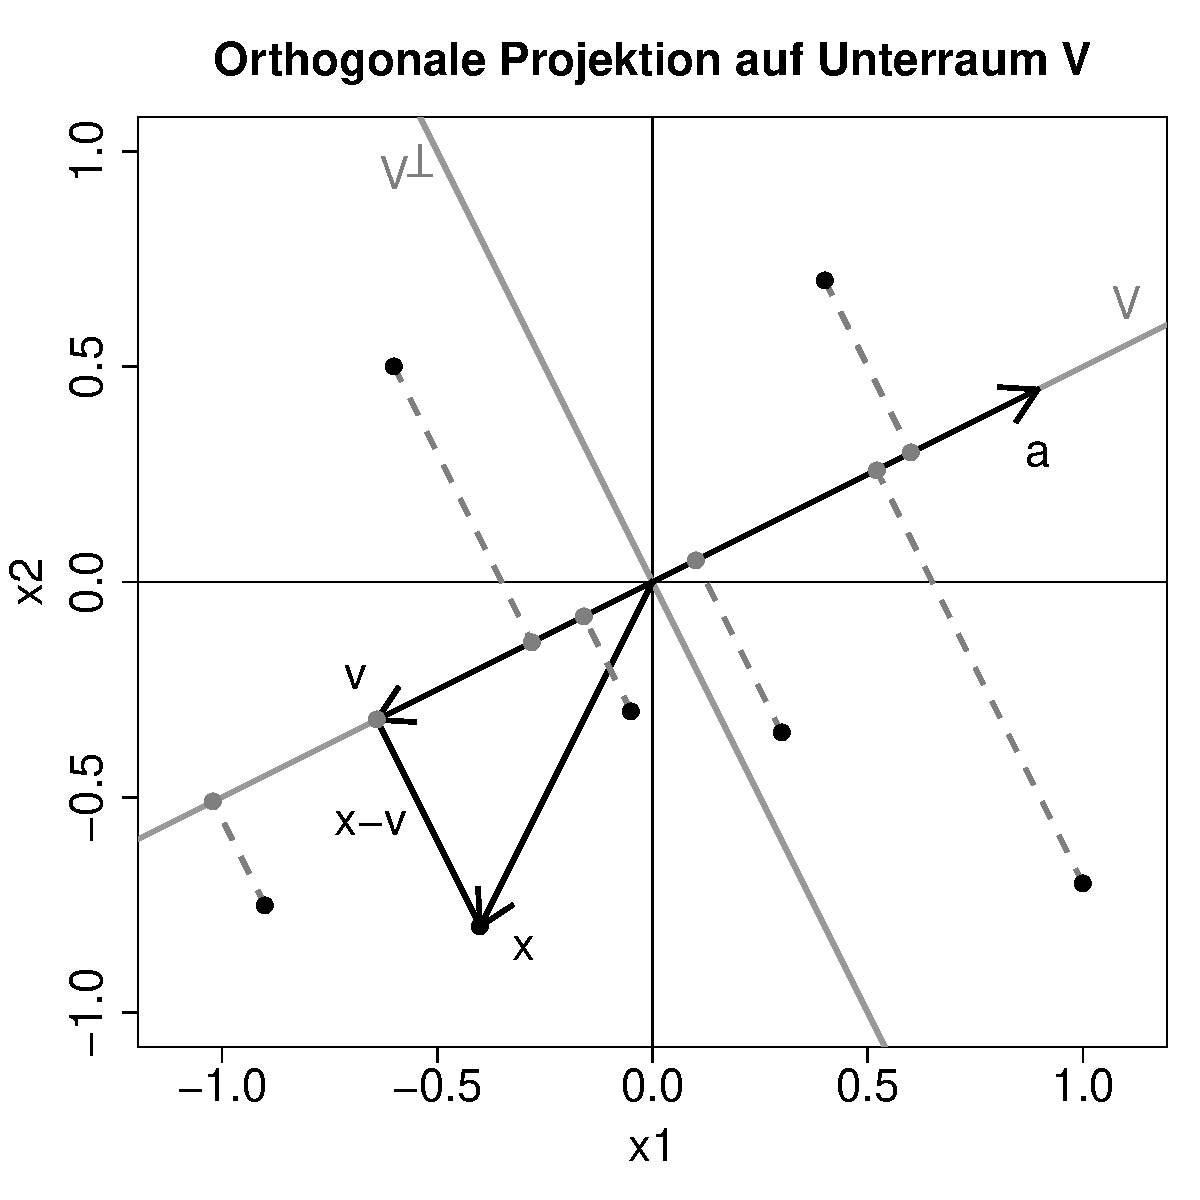
\includegraphics[width=8cm]{orthProj}
\vspace*{-1em}
\caption{Orthogonale Projektion von Vektoren $\bm{x}$ auf Unterraum $V$ mit Basis $\bm{a}$}
\label{fig:orthProj}
\end{figure}

%%%%%%%%%%%%%%%%%%%%%%%%%%%%%%%%%%%%%%%%%%%%%%%%%%%%%%%%%%%%%%%%%%
%%%%%%%%%%%%%%%%%%%%%%%%%%%%%%%%%%%%%%%%%%%%%%%%%%%%%%%%%%%%%%%%%%
\subsubsection{Eigenschaften}
%%%%%%%%%%%%%%%%%%%%%%%%%%%%%%%%%%%%%%%%%%%%%%%%%%%%%%%%%%%%%%%%%%
%%%%%%%%%%%%%%%%%%%%%%%%%%%%%%%%%%%%%%%%%%%%%%%%%%%%%%%%%%%%%%%%%%

Im Fall eines eindimensionalen Unterraums $V$, dessen Basisvektor $\bm{a}$ bereits normiert ist ($\|\bm{a}\|^{2} =  \bm{a}^{\top} \bm{a} = 1$), vereinfacht sich die Projektion zu $\bm{a} \bm{a}^{\top} \bm{x}$, die Koordinaten des projizierten Vektors bzgl.\ $\bm{a}$ liefert entsprechend $\bm{a}^{\top} \bm{x}$ -- das Skalarprodukt von $\bm{a}$ und $\bm{x}$.

Vektoren, die bereits aus $V$ stammen, bleiben durch die Projektion unverändert, insbesondere ist also $\bm{P} \bm{A} = \bm{A}$.\footnote{Ist $\bm{v}$ aus $V$, lässt sich $\bm{v} = \bm{C} \bm{y}$ schreiben, wobei $\bm{y}$ der Koordinatenvektor von $\bm{v}$ bzgl.\ einer Orthogonalbasis $\bm{C}$ von $V$ ist. Damit folgt $\bm{P} \bm{v} = \bm{C} \bm{C}^{\top} \bm{v} = \bm{C} \bm{C}^{\top} \bm{C} \bm{y} = \bm{C} \bm{y} = \bm{v}$.} Orthogonale Projektionen sind idempotent ($\bm{P}^{2} = \bm{P}$) und symmetrisch ($\bm{P}^{\top} = \bm{P})$,\footnote{Zunächst gilt $\bm{P}^{2} = (\bm{C} \bm{C}^{\top}) (\bm{C} \bm{C}^{\top}) = \bm{C} \bm{C}^{\top} = \bm{P}$. Weiter gilt $\bm{P}^{\top} = (\bm{C} \bm{C}^{\top})^{\top} = \bm{C} \bm{C}^{\top} = \bm{P}$.} was sie auch bereits vollständig charakterisiert. Ferner gilt $\text{Rang}(\bm{P}) = \text{Rang}(\bm{A}) = p$, der Dimension von $V$. Zudem ist $\text{Rang}(\bm{P}) = \text{tr}(\bm{P})$.\footnote{$\text{tr}(\bm{P}) = \text{tr}(\bm{C} \bm{C}^{\top}) = \text{tr}(\bm{C}^{\top} \bm{C}) = \text{tr}(\bm{I}) = p$.} $\bm{P}$ besitzt nur die Eigenwerte $1$ mit Vielfachheit $p$ und $0$ mit Vielfachheit $n-p$. Die Eigenvektoren zum Eigenwert $1$ bilden dabei eine Orthogonalbasis von $V$, da Vektoren $\bm{v}$ aus $V$ durch $\bm{P}$ unverändert bleiben. Ist für zwei orthogonale Projektionen $\bm{P}_{1}$ und $\bm{P}_{2}$ ihr Produkt $\bm{P}_{1} \bm{P}_{2}$ symmetrisch, gilt $\bm{P}_{1} \bm{P}_{2} = \bm{P}_{2} \bm{P}_{1}$.\footnote{$\bm{P}_{1} \bm{P}_{2} = (\bm{P}_{1} \bm{P}_{2})^{\top} = \bm{P}_{2}^{\top} \bm{P}_{1}^{\top} = \bm{P}_{2} \bm{P}_{1}$.}

Die Projektion auf das orthogonale Komplement $V^{\perp}$ von $V$ berechnet sich mit der $(n \times n)$-Einheitsmatrix $\bm{I}$ als $\bm{I} - \bm{P}$.\footnote{Ist $\bm{w} = (\bm{I} - \bm{P}) \bm{x}$ aus $V^{\perp}$ und $\bm{v}$ aus $V$, muss $\bm{w}^{\top} \bm{v} = \bm{0}$ gelten. $\bm{v}$ lässt sich als $\bm{v} = \bm{C} \bm{y}$ schreiben, wobei $\bm{y}$ der Koordinatenvektor von $\bm{v}$ bzgl.\ einer Orthogonalbasis $\bm{C}$ von $V$ ist. Nun gilt $\bm{w}^{\top} \bm{v} = ((\bm{I} - \bm{P}) \bm{x})^{\top} \bm{C} \bm{y} = \bm{x}^{\top} (\bm{I} - \bm{P}) \bm{C} \bm{y} = (\bm{x}^{\top} - \bm{x}^{\top} \bm{C} \bm{C}^{\top}) \bm{C} \bm{y} = \bm{x}^{\top} \bm{C} \bm{y} - \bm{x}^{\top} \bm{C} \bm{C}^{\top} \bm{C} \bm{y} = \bm{x}^{\top} \bm{C} \bm{y} - \bm{x}^{\top} \bm{C} \bm{y} = \bm{0}$.} Der Rang von $\bm{I} - \bm{P}$ ist gleich $n - \text{Rang}(\bm{A})$, der Dimension von $V^{\perp}$. Für $\bm{v}$ aus $V$ gilt $(\bm{I} - \bm{P}) \bm{v} = \bm{0}$,\footnote{$(\bm{I}-\bm{P}) \bm{v} = \bm{I} \bm{v} - \bm{P} \bm{v} = \bm{v} - \bm{v} = \bm{0}$, da $\bm{v}$ durch $\bm{P}$ unverändert bleibt.} insbesondere ist also $(\bm{I} - \bm{P}) \bm{A} = \bm{0}$.

%%%%%%%%%%%%%%%%%%%%%%%%%%%%%%%%%%%%%%%%%%%%%%%%%%%%%%%%%%%%%%%%%%
%%%%%%%%%%%%%%%%%%%%%%%%%%%%%%%%%%%%%%%%%%%%%%%%%%%%%%%%%%%%%%%%%%
\subsubsection{Beispiele}
%%%%%%%%%%%%%%%%%%%%%%%%%%%%%%%%%%%%%%%%%%%%%%%%%%%%%%%%%%%%%%%%%%
%%%%%%%%%%%%%%%%%%%%%%%%%%%%%%%%%%%%%%%%%%%%%%%%%%%%%%%%%%%%%%%%%%

Als Beispiel sollen die im vorangehenden Abschnitt simulierten Daten mit der Projektion $\bm{P}_{1}$ im durch die Beobachtungsobjekte aufgespannten $n$-dimensionalen Personenraum auf den eindimensionalen Unterraum projiziert werden, dessen Basisvektor $\bm{1}$ aus lauter $1$-Einträgen besteht. Dies bewirkt, dass alle Werte jeweils durch den Mittelwert der zugehörigen Variable ersetzt werden.\footnote{\label{ftn:ones}$\bm{P}_{1} = \bm{1}_{n} (\bm{1}_{n}^{\top} \bm{1}_{n})^{-1} \bm{1}_{n}^{\top} = \frac{1}{n} \, \bm{1}_{n} \bm{1}_{n}^{\top} = \frac{1}{n} \, \bm{1}_{n \times n}$.} Die Projektion auf das orthogonale Komplement liefert die Differenzen zum zugehörigen Spaltenmittelwert. Damit ist $\bm{I}-\bm{P}_{1}$ gleich der Zentriermatrix (Abschn.\ \ref{sec:matAlg}).
\begin{lstlisting}
> X <- matrix(c(20,26,10,19, 29,27,20,12, 17,23,27,25), nrow=4)

# Basisvektor eines eindimensionalen Unterraums: lauter 1-Einträge
> ones <- rep(1, nrow(X))
> P1   <- ones %*% solve(t(ones) %*% ones) %*% t(ones)     # Projektion
> P1x  <- P1 %*% X         # Koordinaten der Projektion
> head(P1x, n=3)           # Werte ersetzt durch Variablen-Mittelwerte
      [,1]  [,2]  [,3]
[1,] 18.75    22    23
[2,] 18.75    22    23
[3,] 18.75    22    23

> colMeans(X)              # Kontrolle: Spaltenmittel der Daten
[1] 18.75 22.00 23.00

# orthogonale Projektion auf normierten Vektor als Basis des Unterraums
> a  <- ones / sqrt(crossprod(ones))             # normiere Basisvektor
> P2 <- a %*% t(a)         # orthogonale Projektion
> all.equal(P1, P2)        # Kontrolle: Vergleich mit erster Projektion
[1] TRUE

# Projektion auf orthogonales Komplement von P1
> IP1   <- diag(nrow(X)) - P1
> IP1x  <- IP1 %*% X        # zentrierte Daten

# Kontrolle
> all.equal(IP1x, scale(X, center=colMeans(X), scale=FALSE),
+           check.attributes=FALSE)
[1] TRUE
\end{lstlisting}

Als weiteres Beispiel sollen die Daten im durch die Variablen aufgespannten dreidimensionalen Raum auf den zweidimensionalen Unterraum projiziert werden, dessen Basisvektoren die zwei ersten Vektoren der Standardbasis sind. Dies bewirkt, dass die dritte Komponente jedes Zeilenvektors der Datenmatrix auf $0$ gesetzt wird.
\begin{lstlisting}
# Basis eines 2D Unterraums: erste 2 Standard-Basisvektoren
> A   <- cbind(c(1, 0, 0), c(0, 1, 0))
> P3  <- A %*% solve(t(A) %*% A) %*% t(A) # orthogonale Projektion
> Px3 <- t(P3 %*% t(X))                   # Koordinaten der Projektion
> head(Px3, n=3)                          # 3. Komponente auf 0 gesetzt
     [,1]  [,2]  [,3]
[1,]   20    29     0
[2,]   26    27     0
[3,]   10    20     0
\end{lstlisting}

Mit Hilfe der $QR$-Zerlegung lassen sich orthogonale Projektionen numerisch stabiler berechnen als mit der direkten Umsetzung der mathematischen Formel: Mit $\bm{X} = \bm{Q} \bm{R}$ folgt für die Pseudoinverse\index{Matrix!Pseudoinverse} $\bm{X}^{+} = \bm{R}^{-1} \bm{Q}^{\top}$\footnote{Hier sei voller Spaltenrang von $\bm{X}$ vorausgesetzt. Dann ist $\bm{X}^{+} = (\bm{X}^{\top} \bm{X})^{-1} \bm{X}^{\top} = ((\bm{Q} \bm{R})^{\top} \bm{Q} \bm{R})^{-1} (\bm{Q} \bm{R})^{\top} = (\bm{R}^{\top} \bm{Q}^{\top} \bm{Q} \bm{R})^{-1} \bm{R}^{\top} \bm{Q}^{\top} = (\bm{R}^{\top} \bm{R})^{-1} \bm{R}^{\top} \bm{Q}^{\top} = \bm{R}^{-1} \bm{R}^{t -1} \bm{R}^{\top} \bm{Q}^{\top} = \bm{R}^{-1} \bm{Q}^{\top}$.} und für die Projektion (Hat-Matrix $\bm{H}$)\index{allgemeines lineares Modell!Hat-Matrix} $\bm{P} = \bm{Q} \bm{Q}^{\top}$.\footnote{$\bm{X} \bm{X}^{+} = \bm{Q} \bm{R} \bm{R}^{-1} \bm{Q}^{\top} = \bm{Q} \bm{Q}^{\top}$.}
\begin{lstlisting}
> qrX   <- qr(X)                           # QR-Zerlegung
> Q     <- qr.Q(qrX)                       # extrahiere Q
> R     <- qr.R(qrX)                       # extrahiere R
> Xplus <- solve(t(X) %*% X) %*% t(X)      # Pseudoinverse X+
> all.equal(Xplus, solve(R) %*% t(Q))      # X+ = R^(-1) Q^t
[1] TRUE

> all.equal(X %*% Xplus, Q %*% t(Q))       # P = Q Q^t
[1] TRUE
\end{lstlisting}

%%%%%%%%%%%%%%%%%%%%%%%%%%%%%%%%%%%%%%%%%%%%%%%%%%%%%%%%%%%%%%%%%%
%%%%%%%%%%%%%%%%%%%%%%%%%%%%%%%%%%%%%%%%%%%%%%%%%%%%%%%%%%%%%%%%%%
\section{Hauptkomponentenanalyse}
\label{sec:multPCA}
%%%%%%%%%%%%%%%%%%%%%%%%%%%%%%%%%%%%%%%%%%%%%%%%%%%%%%%%%%%%%%%%%%
%%%%%%%%%%%%%%%%%%%%%%%%%%%%%%%%%%%%%%%%%%%%%%%%%%%%%%%%%%%%%%%%%%

\index{Hauptkomponentenanalyse}
Die Hauptkomponentenanalyse dient dazu, die Hauptstreuungsrichtungen multivariater Daten im durch die Variablen aufgespannten Raum zu identifizieren. Hauptkomponenten sind neue Variablen, die als Linearkombinationen der beobachteten Variablen gebildet werden und folgende Eigenschaften besitzen:

\begin{itemize}
\item Die Linearkombinationen sind standardisiert, d.\,h.\ die Koeffizientenvektoren haben jeweils die Länge $1$. Die Koeffizientenvektoren sind die normierten\index{Matrix!Eigenwerte, -vektoren} Eigenvektoren der Kovarianzmatrix der Daten (bis auf potentiell unterschiedliche Vorzeichen i.\,S.\ von Rotationen um $180^{\circ}$) und damit paarweise orthogonal.\footnote{Es sei $\overline{\bm{x}}$ das Zentroid der spaltenweise aus den Variablen zusammengestellten Datenmatrix $\bm{X}$, $\bm{x}$ ein Datenvektor und $\bm{G}$ die Matrix der spaltenweise zusammengestellten normierten Eigenvektoren der Kovarianzmatrix $\bm{S}$ von $\bm{X}$ (Abschn.\ \ref{sec:matProp}). Mit dem Spektralsatz ist $\bm{G}$ eine Orthogonalmatrix ($\bm{G}^{\top} = \bm{G}^{-1}$, s.\ Abschn.\ \ref{sec:matDecomp}). Dann berechnet sich der zugehörige Vektor $\bm{y}$ der Hauptkomponenten als $\bm{y} = \bm{G}^{\top} (\bm{x} - \overline{\bm{x}})$.}
\item Die Hauptkomponenten sind zentriert und paarweise unkorreliert.\footnote{Genauer gesagt ist ihre Kovarianz $0$ -- da ihre Varianz auch $0$ sein kann, ist die Korrelation nicht immer definiert. $\bm{S}$ lässt sich mit $\bm{S} = \bm{G} \bm{D} \bm{G}^{\top}$ diagonalisieren (Abschn.\ \ref{sec:matDecomp}). Dabei ist $\bm{D}$ die zu $\bm{G}$ gehörende, aus den Eigenwerten von $\bm{S}$ gebildete Diagonalmatrix. Damit gilt $V(\bm{y}) = V(\bm{G}^{\top} (\bm{x} - \overline{\bm{x}})) = V(\bm{G}^{\top} \bm{x} - \bm{G}^{\top} \overline{\bm{x}}) = V(\bm{G}^{\top} \bm{x}) = \bm{G}^{\top} V(\bm{x}) \bm{G} = \bm{G}^{\top} \bm{S} \bm{G} = \bm{G}^{\top} \bm{G} \bm{D} \bm{G}^{\top} \bm{G} = \bm{D}$. Die Varianzen der Hauptkomponenten sind also gleich den Eigenwerten der Kovarianzmatrix der Daten, die Kovarianzen sind $0$.}
\item Der euklidische Abstand zwischen zwei Punkten im Raum der Hauptkomponenten ist derselbe wie im Raum der beobachteten Variablen.\footnote{Es seien $\bm{x}_{1}$ und $\bm{x}_{2}$ zwei Datenvektoren mit zugehörigen Hauptkomponenten-Vektoren $\bm{y}_{1}$ und $\bm{y}_{2}$. Dann gilt $\|\bm{x}_{2} - \bm{x}_{1}\|^{2} = (\bm{x}_{2} - \bm{x}_{1})^{\top} (\bm{x}_{2} - \bm{x}_{1}) = (\bm{x}_{2} - \bm{x}_{1})^{\top} \bm{G} \bm{G}^{\top} (\bm{x}_{2} - \bm{x}_{1}) = (\bm{G}^{\top} (\bm{x}_{2} - \bm{x}_{1}))^{\top} \bm{G}^{\top} (\bm{x}_{2} - \bm{x}_{1}) = \|\bm{G}^{\top} (\bm{x}_{2} - \bm{x}_{1})\|^{2} = \|\bm{G}^{\top} \bm{x}_{2} - \bm{G}^{\top} \bm{x}_{1}\|^{2} = \|\bm{G}^{\top} (\bm{x}_{2} - \overline{\bm{x}}) - \bm{G}^{\top} (\bm{x}_{1} - \overline{\bm{x}})\|^{2} = \|\bm{y}_{2} - \bm{y}_{1} \|^{2}$.}
\item Die Streuung der Hauptkomponenten ist im folgenden Sinn sukzessive maximal: Die erste Hauptkomponente ist diejenige unter allen standardisierten Linearkombinationen mit der größten Streuung. Unter allen standardisierten Linearkombinationen, die mit der ersten Hauptkomponente unkorreliert sind, ist die zweite Hauptkomponente dann wieder diejenige mit der größten Streuung. Für die weiteren Hauptkomponenten gilt dies analog.
\end{itemize}

%%%%%%%%%%%%%%%%%%%%%%%%%%%%%%%%%%%%%%%%%%%%%%%%%%%%%%%%%%%%%%%%%%
%%%%%%%%%%%%%%%%%%%%%%%%%%%%%%%%%%%%%%%%%%%%%%%%%%%%%%%%%%%%%%%%%%
\subsection{Berechnung}
\label{sec:pcaCalc}
%%%%%%%%%%%%%%%%%%%%%%%%%%%%%%%%%%%%%%%%%%%%%%%%%%%%%%%%%%%%%%%%%%
%%%%%%%%%%%%%%%%%%%%%%%%%%%%%%%%%%%%%%%%%%%%%%%%%%%%%%%%%%%%%%%%%%

\index[func]{prcomp()@\lstinline{prcomp()}}
\index[func]{princomp()@\lstinline{princomp()}}
Für die Berechnung der Hauptkomponenten samt ihrer jeweiligen Streuung stehen \lstinline!prcomp()! und \lstinline!princomp()! zur Verfügung.
\begin{lstlisting}
  prcomp(<<Matrix oder Modellformel>>, scale=FALSE, data=<<Datensatz>>)
princomp(<<Matrix oder Modellformel>>,              data=<<Datensatz>>,
         cor=FALSE, covmat)
\end{lstlisting}

In der ersten Variante akzeptieren bei Funktionen die spaltenweise aus den Variablen zusammengestellte Datenmatrix. Damit die Hauptkomponenten aus den standardisierten Variablen berechnet werden, ist \lstinline!prcomp(..., scale=TRUE)! bzw.\ \lstinline!princomp(..., cor=TRUE)! zu setzen. Alternativ lassen sich die Variablen in beiden Funktionen als rechte Seite einer Modellformel nennen. Stammen sie aus einem Datensatz, muss dieser unter \lstinline!data! übergeben werden. \lstinline!princomp()! erlaubt es zusätzlich, die Kovarianzmatrix der Daten über das Argument \lstinline!covmat! separat zu spezifizieren, etwa um direkt eine \index{robuste Verfahren!Hauptkomponentenanalyse} robuste Schätzung der theoretischen Kovarianzmatrix zu verwenden (Abschn.\ \ref{sec:varRob}).\footnote{Für die robuste Hauptkomponentenanalyse s.\ das Paket \lstinline!pcaPP!\index[pack]{pcaPP@\lstinline{pcaPP}} \cite{Filzmoser2011a}.}
\begin{lstlisting}
> sigma <- matrix(c(4,2, 2,3), ncol=2)  # 2x2 Kovarianzmatrix
> mu    <- c(1, 2)                      # Zentroid für Zufallsvektoren
> N     <- 50                           # Anzahl Personen
> library(mvtnorm)                      # für rmvnorm()
> X     <- rmvnorm(N, mean=mu, sigma=sigma)   # Multinormalverteilung
> (pca  <- prcomp(X))                   # Hauptkomponentenanalyse
Standard deviations:
[1] 2.436560 1.270408

Rotation:
            PC1         PC2
[1,] -0.7335078   0.6796810
[2,] -0.6796810  -0.7335078
\end{lstlisting}

Die Ausgabe von \lstinline!prcomp()! ist eine Liste mit zwei Komponenten: die erste enthält den Vektor der korrigierten Streuungen der Hauptkomponenten (Überschrift \lstinline!Standard deviations!). Dies sind gleichzeitig die Wurzeln aus den Eigenwerten der korrigierten Kovarianzmatrix der Daten (Abschn.\ \ref{sec:matProp}). Die zweite Komponente beinhaltet die als Spalten einer Matrix $\bm{G}$ zusammengestellten Koeffizienten der Linearkombinationen zur Bildung der Hauptkomponenten (Überschrift \lstinline!Rotation!). Dies sind gleichzeitig die normierten Eigenvektoren der korrigierten Kovarianzmatrix.
\begin{lstlisting}
> eig    <- eigen(cov(X))       # Eigenwerte, -vektoren Kovarianzmatrix
> eigVal <- eig$values          # Eigenwerte
> sqrt(eigVal)                  # deren Wurzel = Streuungen der HK
[1] 2.436560 1.270408

# normierte Eigenvektoren = Koeffizientenvektoren Linearkombinationen
> (G <- eig$vectors)
           [,1]        [,2]
[1,] -0.7335078   0.6796810
[2,] -0.6796810  -0.7335078
\end{lstlisting}

Die Hauptkomponenten kann man in einem Koordinatensystem ablesen, das seinen Ursprung im Zentroid der Daten hat. Die Achsen weisen in Richtung der Koeffizientenvektoren und haben dieselbe Einheit wie das Standard-Koordinatensystem (Abb.\ \ref{fig:pca}). Die Hauptkomponenten sind die orthogonale Projektion der zentrierten Daten auf die Geraden in Richtung der Eigenvektoren der Kovarianzmatrix (Abschn.\ \ref{sec:matOrthProj}). Die Streuung der projizierten Daten entlang der Geraden ist daher gleich der Streuung der zugehörigen Hauptkomponente. Sie ist zudem gleich der Wurzel aus dem entsprechenden Eigenwert der Kovarianzmatrix.
\begin{lstlisting}
# normierte Eigenvektoren * Wurzel aus zugehörigem Eigenwert
> B    <- G %*% diag(sqrt(eigVal))
> ctr  <- colMeans(X)                                 # Zentroid
> xMat <- rbind(ctr[1] - B[1, ], ctr[1])
> yMat <- rbind(ctr[2] - B[2, ], ctr[2])

# Punkt-Steigungsform der durch Eigenvektoren definierten Achsen
> ab1 <- solve(cbind(1, xMat[ , 1]), yMat[ , 1])      # Achse 1
> ab2 <- solve(cbind(1, xMat[ , 2]), yMat[ , 2])      # Achse 2

# Daten im Streudiagramm darstellen
> plot(X, xlab="x", ylab="y", pch=20, asp=1,
+      main="Datenwolke und Hauptkomponenten")

> abline(coef=ab1, lwd=2, col="gray")                 # Achse 1
> abline(coef=ab2, lwd=2, col="gray")                 # Achse 2
> matlines(xMat, yMat, lty=1, lwd=6, col="blue")      # Streuungen HK
> points(ctr[1], ctr[2], pch=16, col="red", cex=3)    # Zentroid

# Legende einfügen
> legend(x="topleft", legend=c("Daten", "Achsen HK",
+        "Streuungen HK", "Zentroid"), pch=c(20, NA, NA, 16),
+        lty=c(NA, 1, 1, NA), col=c("black", "gray", "blue", "red"))
\end{lstlisting}

\begin{figure}[ht]
\centering
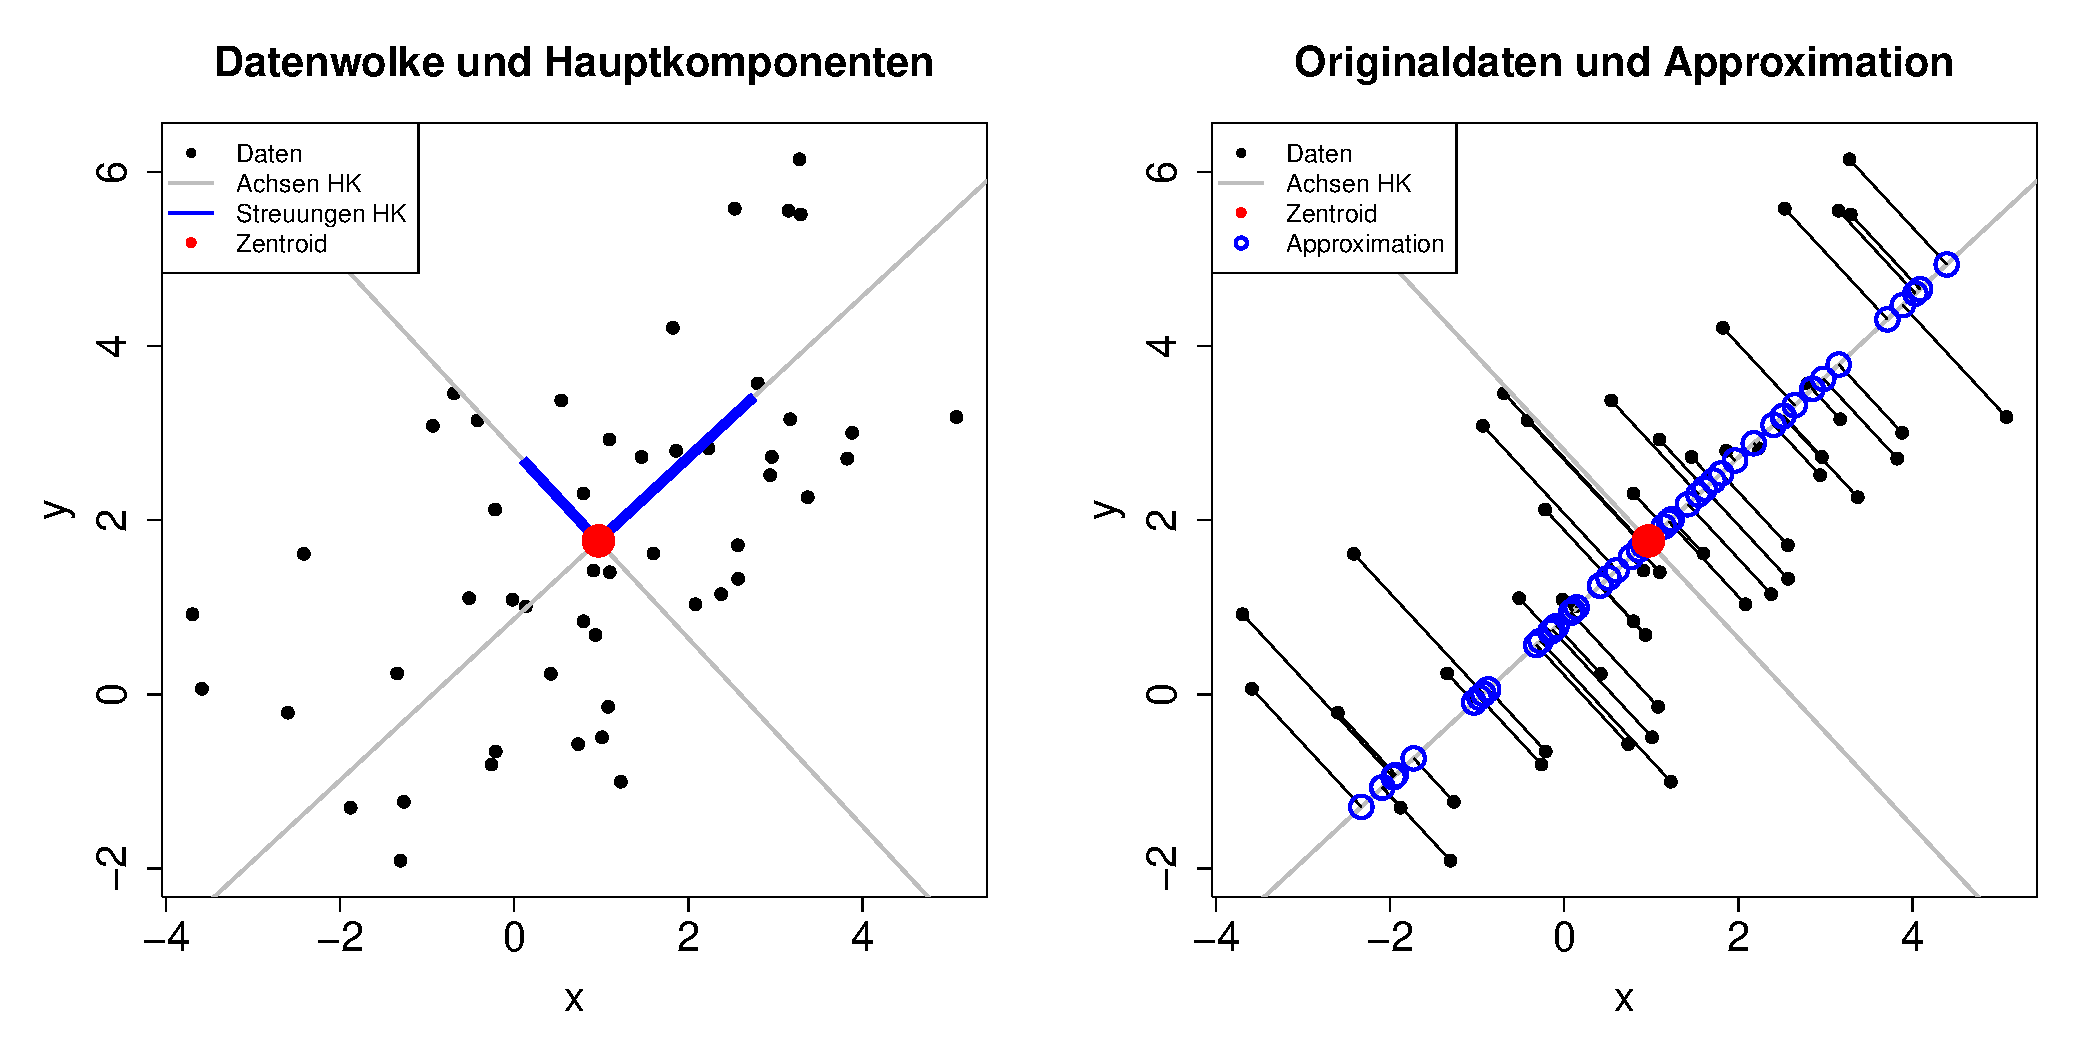
\includegraphics[width=12.5cm]{pcaAxes}
\vspace*{-1em}
\caption{Hauptkomponentenanalyse: Koordinatensystem mit Achsen in Richtung der ins Zentroid verschobenen Eigenvektoren sowie Streuungen der Hauptkomponenten. Originaldaten und Approximation durch erste Hauptkomponente}
\label{fig:pca}
\end{figure}

Aus der Matrix $\bm{G}$ der Koeffizienten der standardisierten Linearkombinationen und der spaltenweise zentrierten Datenmatrix $\dot{\bm{X}}$ berechnen sich die Hauptkomponenten als neue Variablen durch $\dot{\bm{X}} \bm{G}$. Man erhält sie mit \lstinline!predict(<<PCA>>)!.\footnote{\label{ftn:pcamds}Das Ergebnis ist -- bis auf mögliche Spiegelung der Achsen -- identisch mit dem der metrischen multidimensionalen Skalierung (Abschn.\ \ref{sec:multMDS}) mit \lstinline!cmdscale(dist(X))!.} Dabei ist \lstinline!<<PCA>>! das Ergebnis einer Hauptkomponentenanalyse mit \lstinline!prcomp()! oder \lstinline!princomp()!. 
\begin{lstlisting}
> Y <- predict(pca)                     # Hauptkomponenten
> head(Y, n=3)
     PC1       PC2
[1,] -4.257878 -1.171098
[2,] -1.021898 -0.370420
[3,]  1.500310  1.683688

> (Ysd <- apply(Y, 2, sd))              # deren Streuungen
     PC1       PC2
2.436560  1.270408

# Kontrolle
> Xdot    <- scale(X, center=TRUE, scale=FALSE)     # zentrierte Daten
> Y_XdotG <- Xdot %*% G                 # Hauptkomponenten
> head(Y_XdotG, n=3)
           PC1        PC2
[1,] -4.257878  -1.171098
[2,] -1.021898  -0.370420
[3,]  1.500310   1.683688
\end{lstlisting}

Mit der Singulärwertzerlegung von $\dot{\bm{X}}$ (Abschn.\ \ref{sec:matDecomp}) ergeben sich die Hauptkomponenten auch als spaltenweise aus den Links-Singulärvektoren zusammengestellte Matrix $\bm{u}$, deren Spalten mit den Singulärwerten skaliert wurden.
\begin{lstlisting}
> svd_Xdot <- svd(Xdot)                 # Singulärwertzerlegung
> Y_svd    <- svd_Xdot$u %*% diag(svd_Xdot$d)       # Hauptkomponenten
> head(Y_svd, n=3)                      # ...
\end{lstlisting}

Bei \lstinline!predict(<<PCA>>)! lässt sich für das Argument \lstinline!newdata! eine Matrix mit neuen Werten der ursprünglichen Variablen angeben, die dann in Werte auf den Hauptkomponenten umgerechnet werden.
\begin{lstlisting}
# Hauptkomponenten für neue Daten berechnen
> Xnew <- matrix(1:4, ncol=2)
> predict(pca, newdata=Xnew)
            PC1        PC2
[1,] -0.8672799 -0.8858317
[2,] -2.2804688 -0.9396585
\end{lstlisting}

Die Streuungen der Hauptkomponenten, den Anteil ihrer Varianz an der Gesamtvarianz (i.\,S.\ der Spur der Kovarianzmatrix der Daten) sowie den kumulativen Anteil der Varianz der Hauptkomponenten an der Gesamtvarianz gibt \lstinline!summary(<<PCA>>)!\index[func]{summary()@\lstinline{summary()}} aus.
\begin{lstlisting}
> summary(pca)
Importance of components:
                          PC1     PC2
Standard deviation     2.4366  1.2704
Proportion of Variance 0.7863  0.2137
Cumulative Proportion  0.7863  1.0000

# Kontrolle: Anteil der Varianz der HK an Gesamtvarianz
> Ysd^2 / sum(diag(cov(X)))
[1] 0.7862549  0.2137451
\end{lstlisting}

%%%%%%%%%%%%%%%%%%%%%%%%%%%%%%%%%%%%%%%%%%%%%%%%%%%%%%%%%%%%%%%%%%
%%%%%%%%%%%%%%%%%%%%%%%%%%%%%%%%%%%%%%%%%%%%%%%%%%%%%%%%%%%%%%%%%%
\subsection{Dimensionsreduktion}
\label{sec:pcaDimReduce}
%%%%%%%%%%%%%%%%%%%%%%%%%%%%%%%%%%%%%%%%%%%%%%%%%%%%%%%%%%%%%%%%%%
%%%%%%%%%%%%%%%%%%%%%%%%%%%%%%%%%%%%%%%%%%%%%%%%%%%%%%%%%%%%%%%%%%

Häufig dient die Hauptkomponentenanalyse der Datenreduktion: Wenn von Beobachtungsobjekten Werte von sehr vielen Variablen vorliegen, ist es oft wünschenswert, diese Daten durch Werte von weniger Variablen möglichst gut zu approximieren. Als Kriterium dient dabei die Summe der quadrierten Abstände zwischen Originaldaten und Approximation. Eine perfekte Reproduktion der Originaldaten lässt sich zunächst wie folgt erreichen: Sei die \emph{Ladungs-Matrix} $\bm{B}$ spaltenweise aus den Koeffizientenvektoren der Hauptkomponenten zusammengestellt. Zusätzlich sollen die Spalten von $\bm{B}$ als Länge die Streuung der jeweils zugehörigen Hauptkomponente besitzen, was mit $\bm{B} = \bm{G} \bm{D}^{\frac{1}{2}}$ erreicht wird. Weiter sei $\bm{H}$ die \emph{Score-Matrix} der standardisierten Hauptkomponenten, die jeweils Mittelwert $0$ und Varianz $1$ besitzen. Ferner sei $\overline{\bm{x}}$ das Zentroid der Originaldaten. Für die Datenmatrix $\bm{X}$ gilt dann $\bm{X} = \bm{H} \bm{B}^{\top} + \overline{\bm{x}}$.\footnote{Zunächst gilt $\bm{H} = \bm{Y} \bm{D}^{-\frac{1}{2}}$, wobei $\bm{Y} = \dot{\bm{X}} \bm{G} = \bm{Z} \bm{X} \bm{G}$ die Matrix der (zentrierten) Hauptkomponenten und $\bm{Z}$ die Zentriermatrix zu $\bm{X}$ ist (Abschn.\ \ref{sec:matAlg}). Wegen $\bm{G}^{\top} = \bm{G}^{-1}$ folgt $\bm{H} \bm{B}^{\top} + \overline{\bm{x}} = \bm{Y} \bm{D}^{-\frac{1}{2}} (\bm{G} \bm{D}^{\frac{1}{2}})^{\top} + \overline{\bm{x}} = \bm{Z} \bm{X} \bm{G} \bm{D}^{-\frac{1}{2}} \bm{D}^{\frac{1}{2}} \bm{G}^{\top} + \overline{\bm{x}} = \dot{\bm{X}} \bm{G} \bm{G}^{\top} + \overline{\bm{x}} = \bm{X}$.}
\begin{lstlisting}
> B  <- G %*% diag(sqrt(eigVal))
> H  <- scale(Y)          # Score-Matrix = standard. Hauptkomponenten
> HB <- H %*% t(B)        # H * B^t

# Reproduktion der Originaldaten: addiere Zentroid c: H * B^t + c
> repr <- sweep(HB, 2, ctr, "+")
> all.equal(X, repr)      # Kontrolle: Übereinstimmung mit X
[1] TRUE
\end{lstlisting}

Sollen die ursprünglichen Daten nun im obigen Sinne optimal durch weniger Variablen repräsentiert werden, können die Spalten von $\bm{B}$ von rechts kommend nacheinander gestrichen werden, wodurch sich etwa eine Matrix $\bm{B}'$ ergibt. Ebenso sind die zugehörigen standardisierten Hauptkomponenten, also die Spalten von $\bm{H}$, zu streichen, wodurch die Matrix $\bm{H}'$ entsteht. Die approximierten Daten $\bm{X}' = \bm{H}' \bm{B}'^{\top} + \overline{\bm{x}}$ liegen dann in einem affinen Unterraum mit niedrigerer Dimension als die ursprünglichen Daten (Abb.\ \ref{fig:pca}).\footnote{Die mittlere Summe der quadrierten Abstände von $\bm{X}$ und $\bm{X}'$ ist gleich der Summe der $q$ kleinsten Eigenwerte der Kovarianzmatrix $\bm{S}$, wenn $q$ Spalten von $\bm{B}$ gestrichen wurden.}
\begin{lstlisting}
# approximiere Originaldaten durch niedrig-dimensionale Daten
> HB1   <- H[ , 1, drop=FALSE] %*% t(B[ , 1, drop=FALSE]) # H' * B'^t
> repr1 <- sweep(HB1, 2, ctr, "+") # H' * B'^t + c
> sum((X-repr1)^2)                 # Summe der quadrierten Abweichungen
[1] 79.08294

# approximierte Daten liegen in eindimensionalem Unterraum
> qr(scale(repr1, center=TRUE, scale=FALSE))$rank
[1] 1

# grafische Darstellung der Originaldaten und der Approximation
> plot(X, xlab="x", ylab="y", pch=20, asp=1,
+      main="Originaldaten und Approximation")

> abline(coef=ab1, lwd=2, col="gray")                   # Achse 1
> abline(coef=ab2, lwd=2, col="gray")                   # Achse 2
> segments(X[ , 1], X[ , 2], repr1[ , 1], repr1[ , 2])
> points(repr1, pch=1, lwd=2, col="blue", cex=2)        # Approximation
> points(ctr[1], ctr[2], pch=16, col="red", cex=3)      # Zentroid

# Legende einfügen
> legend(x="topleft", legend=c("Daten", "Achsen HK",
+        "Zentroid", "Approximation"), pch=c(20, NA, 16, 1),
+        lty=c(NA, 1, NA, NA), col=c("black", "gray", "red", "blue"))
\end{lstlisting}

Die Kovarianzmatrix der Daten lässt sich als $\bm{S} = \bm{B} \bm{B}^{\top}$ zerlegen\footnote{$\bm{B} \bm{B}^{\top} = \bm{G} \bm{D}^{\frac{1}{2}} (\bm{G} \bm{D}^{\frac{1}{2}})^{\top} = \bm{G} \bm{D}^{\frac{1}{2}} \bm{D}^{\frac{1}{2}} \bm{G}^{\top} = \bm{G} \bm{D} \bm{G}^{\top} = \bm{S}$.} (Abschn.\ \ref{sec:matDecomp}). Die Reproduktion von $\bm{S}$ durch die um rechte Spalten gestrichene Matrix $\bm{B}'$ mit $\bm{B}' \bm{B}'^{\top}$ wird schlechter, bleibt aber optimal im Vergleich zu allen anderen Matrizen gleicher Dimensionierung.
\begin{lstlisting}
> cov(X)                   # Kovarianzmatrix von X
         [,1]      [,2]
[1,] 3.939795  2.155180
[2,] 2.155180  3.610964

> B %*% t(B)               # reproduziert Kovarianzmatrix ...
> B[ , 1] %*% t(B[ , 1])   # approximiere Kovarianzmatrix mit B' * B'^t
         [,1]      [,2]
[1,] 3.194211  2.959811
[2,] 2.959811  2.742612
\end{lstlisting}

Die von\index[func]{princomp()@\lstinline{princomp()}} \lstinline!princomp()! berechnete Hauptkomponentenanalyse unterscheidet sich von der durch \lstinline!prcomp()! erzeugten in den ausgegebenen Streuungen: bei \lstinline!prcomp()! sind dies die korrigierten, bei \lstinline!princomp()! die unkorrigierten. Die Streuungen sind gleich den zugehörigen Eigenwerten der unkorrigierten Kovarianzmatrix der Daten.\footnote{Weiterhin basiert \lstinline!prcomp()! intern auf der\index{Matrix!Singulärwertzerlegung} Singulärwertzerlegung der Datenmatrix $\bm{X}$, \lstinline!princomp()! hingegen auf der Spektralzerlegung der Kovarianzmatrix $\bm{S}$ der Daten (Abschn.\ \ref{sec:matDecomp}). Die Singulärwertzerlegung der Datenmatrix gilt als numerisch stabiler bei schlecht konditionierten Matrizen i.\,S.\ der Kondition $\kappa$ (Abschn.\ \ref{sec:matProp}), kann aber langsamer sein. \lstinline!prcomp()! sollte meist vorgezogen werden.} In der Ausgabe von \lstinline!princomp()! sind die Koeffizienten der standardisierten Linearkombination zunächst nicht mit aufgeführt, befinden sich jedoch in der Komponente \lstinline!loadings! der zurückgelieferten Liste.
\begin{lstlisting}
> (pcaPrin <- princomp(X))
Call:
princomp(x = X)
Standard deviations:
  Comp.1    Comp.2
2.412071  1.257640
2 variables and 50 observations.

# Kontrolle: unkorrigierte Streuungen der Hauptkomponenten
> Sml <- cov.wt(pc, method="ML")$cov
> sqrt(diag(Sml))
     PC1       PC2
2.412071  1.257640

> pcaPrin$loadings                         # Koeffizientenmatrix ...
\end{lstlisting}

%%%%%%%%%%%%%%%%%%%%%%%%%%%%%%%%%%%%%%%%%%%%%%%%%%%%%%%%%%%%%%%%%%
%%%%%%%%%%%%%%%%%%%%%%%%%%%%%%%%%%%%%%%%%%%%%%%%%%%%%%%%%%%%%%%%%%
\subsection{Visualisierung}
\label{sec:pcaDiag}
%%%%%%%%%%%%%%%%%%%%%%%%%%%%%%%%%%%%%%%%%%%%%%%%%%%%%%%%%%%%%%%%%%
%%%%%%%%%%%%%%%%%%%%%%%%%%%%%%%%%%%%%%%%%%%%%%%%%%%%%%%%%%%%%%%%%%

Die Varianzen der Hauptkomponenten werden häufig in einem Liniendiagramm (Abschn.\ \ref{sec:plot}) als\index{Grafik!Scree-Plot}\index{Scree-Plot|see{Grafik}} Scree-Plot dargestellt, der mit \lstinline!plot(<<PCA>>, type="b")! aufzurufen ist (Abb.\ \ref{fig:pcaScreeBiplot}). Dabei ist \lstinline!<<PCA>>! das Ergebnis einer Hauptkomponentenanalyse mit \lstinline!prcomp()! oder \lstinline!princomp()!. Für eine grafische Veranschaulichung der Hauptkomponenten selbst über die Hauptachsen des die gemeinsame Verteilung der Daten charakterisierenden Streuungsellipsoids s.\ Abschn.\ \ref{sec:distr2var}, Abb.\ \ref{fig:distr2var}. Ein mit \lstinline!biplot(<<PCA>>)! \index[func]{biplot()@\lstinline{biplot()}} erzeugter Biplot stellt die ersten beiden Hauptkomponenten und die Ladungs-Matrix gleichzeitig in einem Diagramm dar, das eine inhaltliche Interpretation der Hauptkomponentenanalyse fördern soll (Abb.\ \ref{fig:pcaScreeBiplot}). Die Definition eines Biplots ist nicht ganz einheitlich und kann zwischen je nach Software leicht unterschiedlich ausfallen, s.\ \lstinline!?biplot!.
\begin{lstlisting}
> plot(pca, type="b")                    # Scree-Plot
> biplot(pca)                            # stelle Biplot dar
\end{lstlisting}

\begin{figure}[ht]
\centering
%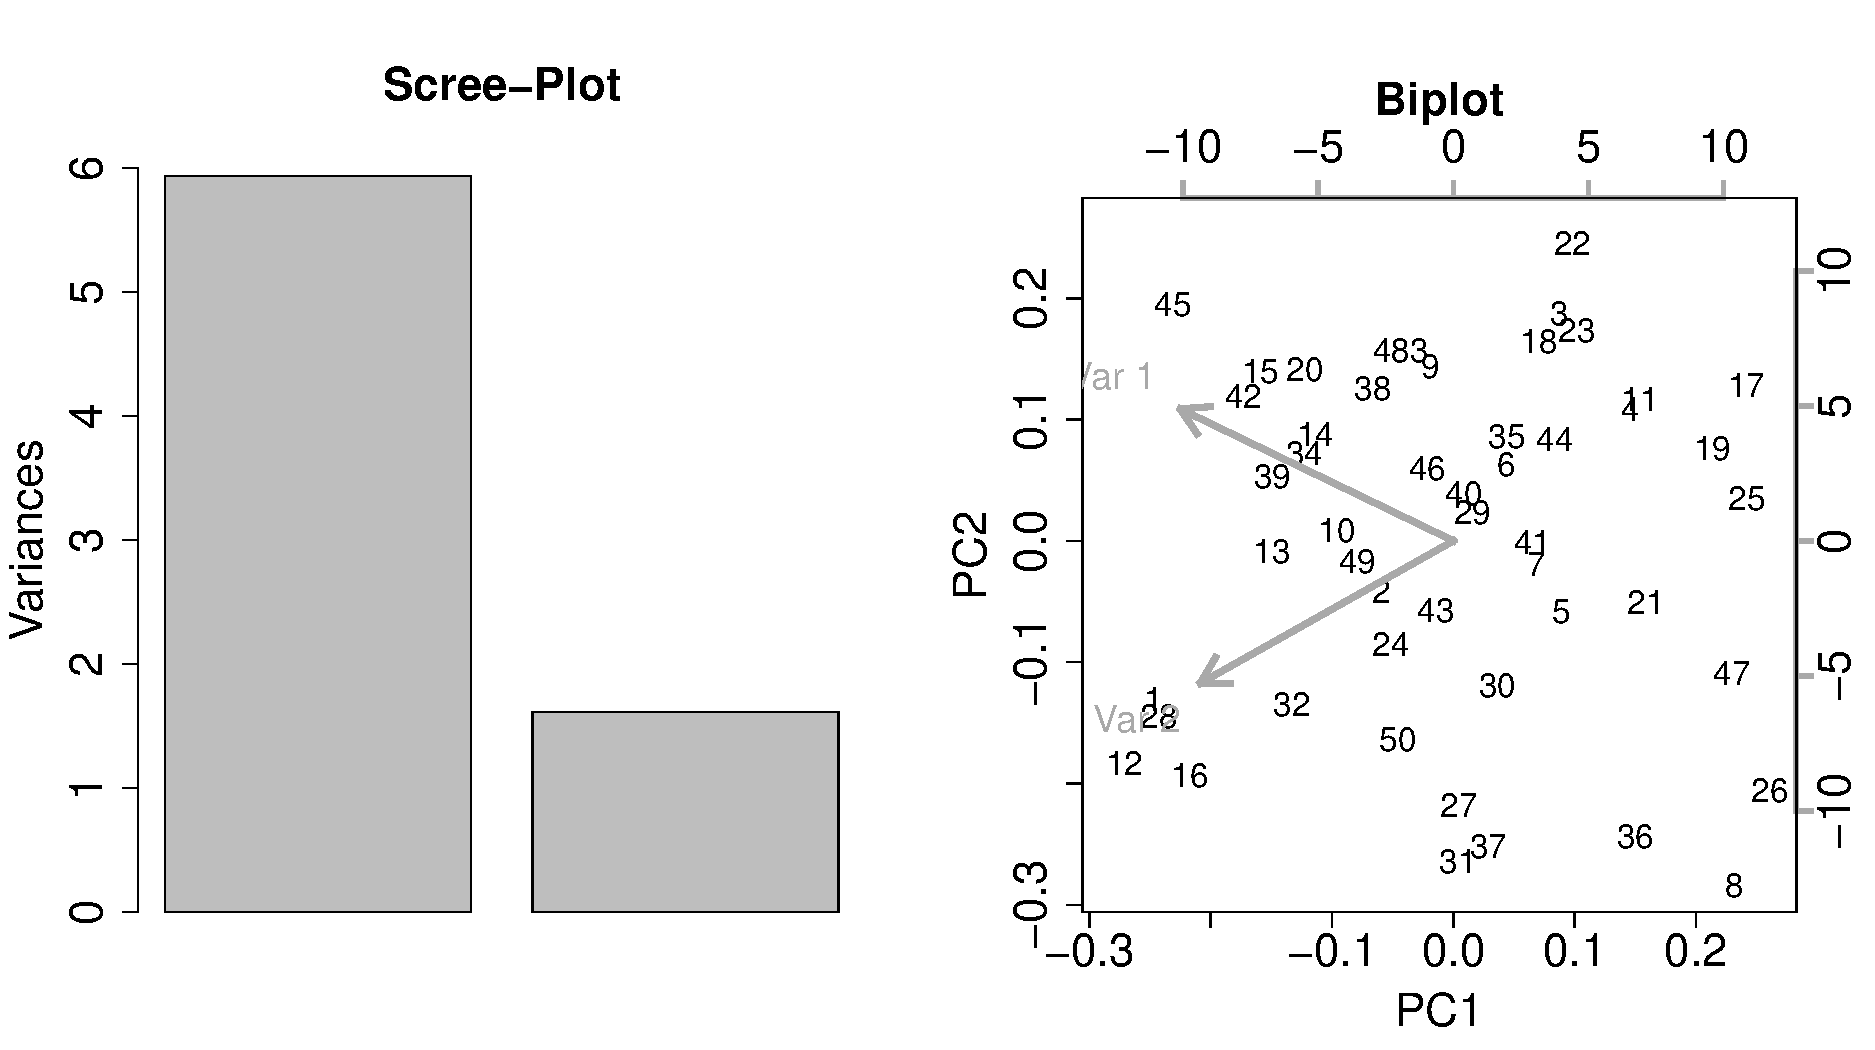
\includegraphics[width=8cm]{pcaScreeBiplot}
\vspace*{-0.5em}
\caption{Scree-Plot und Biplot zur Visualisierung der Ergebnisse einer Hauptkomponentenanalyse}
\label{fig:pcaScreeBiplot}
\end{figure}
     
Für die Darstellung im Biplot werden die Spalten der Hauptkomponenten $\bm{Y}$ mit dem Vektor $1/\bm{f}$ skaliert. Dabei ist $\bm{f}$ gleich den Singulärwerten von $\dot{\bm{X}}$, also gleich der Wurzel aus den Eigenwerten der Kovarianzmatrix von $\bm{X}$ multipliziert mit der Wurzel aus der Anzahl an Beobachtungen. Zur Darstellung der Variablen werden die zugehörigen normierten Eigenvektoren, gleich den Rechts-Singulärvektoren von $\dot{\bm{X}}$, mit $\bm{f}$ skaliert.
\begin{lstlisting}
> (f <- svd_Xdot$d)                      # Skalierungsfaktor
[1] 17.229078  8.983144

> sqrt(eigVal)*sqrt(N)                   # Kontrolle
[1] 17.229078  8.983144

> head(Y %*% diag(1/f), n=3)             # Koordinaten HK für Biplot
            [,1]        [,2]
[1,] -0.24713328 -0.13036620
[2,] -0.05931238 -0.04123501
[3,]  0.08708010  0.18742743

> G %*% diag(f)                          # Koord. Variablen für Biplot 
          [,1]      [,2]
[1,] -12.51065  6.044307
[2,] -11.59258 -6.522982
\end{lstlisting}
     
%%%%%%%%%%%%%%%%%%%%%%%%%%%%%%%%%%%%%%%%%%%%%%%%%%%%%%%%%%%%%%%%%%
%%%%%%%%%%%%%%%%%%%%%%%%%%%%%%%%%%%%%%%%%%%%%%%%%%%%%%%%%%%%%%%%%%
\section{Faktorenanalyse}
\label{sec:multFA}
%%%%%%%%%%%%%%%%%%%%%%%%%%%%%%%%%%%%%%%%%%%%%%%%%%%%%%%%%%%%%%%%%%
%%%%%%%%%%%%%%%%%%%%%%%%%%%%%%%%%%%%%%%%%%%%%%%%%%%%%%%%%%%%%%%%%%

\index{Faktorenanalyse}
Der Faktorenanalyse liegt die Vorstellung zugrunde, dass sich die korrelativen Zusammenhänge zwischen vielen beobachtbaren Merkmalen $X_{j}$ (mit $j = 1, \ldots, p$) aus wenigen latenten Variablen\index{Variable!latente} $F_{k}$ (den \emph{Faktoren} mit $k = 1, \ldots, q$) speisen, die ursächlich auf die Ausprägung der $X_{j}$ wirken.\footnote{\label{ftn:structEqMod}Für weitere Verfahren, die die Beziehungen latenter und beobachtbarer Variablen modellieren, vgl.\ den Abschnitt \emph{Psychometric Models} der CRAN Task Views \cite{CRANtvPsych}. Lineare Strukturgleichungsmodelle\index{lineare Strukturgleichungsmodelle} werden durch die Pakete\index[pack]{sem@\lstinline{sem}}\index[pack]{OpenMx@\lstinline{OpenMx}}\index[pack]{lavaan@\lstinline{lavaan}}\index[pack]{psych@\lstinline{psych}} \lstinline!lavaan! \cite{Rosseel2012}, \lstinline!OpenMx! \cite{Boker2010} und \lstinline!sem! \cite{Fox2009b} -- mit ergänzenden Funktionen in \lstinline!psych! -- unterstützt.} Die Wirkungsweise wird dabei als linear angenommen, d.\,h.\ die $X_{j}$ sollen sich als Linearkombination der $F_{k}$ zzgl.\ eines zufälligen Fehlers ergeben.\footnote{In diesem Sinne ist die Faktorenanalyse das Gegenteil der Hauptkomponentenanalyse, in der die Hauptkomponenten Linearkombinationen der beobachtbaren Variablen sind.} Weiterhin beruht die Faktorenanalyse auf der Annahme, dass sich bei unterschiedlichen Beobachtungsobjekten zwar die Ausprägungen der $F_{k}$ unterscheiden, die den Einfluss der Faktoren auf die $X_{j}$ charakterisierenden Koeffizienten der Linearkombinationen dagegen fest, also für alle Beobachtungsobjekte gleich sind.

Zur Vereinbarung der Terminologie sei $\bm{x}$ der $p$-Vektor der beobachtbaren Merkmalsausprägungen einer Person, $\bm{f}$ der $q$-Vektor ihrer Faktorausprägungen, $\bm{\epsilon}$ der $p$-Vektor der Fehler und $\bm{\Lambda}$ die $(p \times q)$-\emph{Ladungsmatrix} der zeilenweise zusammengestellten Koeffizienten der Linearkombinationen für jedes $X_{j}$. Das Modell geht von standardisierten $X_{j}$ und $F_{k}$ aus, die also Erwartungswert $0$ und Varianz $1$ besitzen sollen. Weiterhin sollen die Fehler untereinander und mit den Faktoren unkorreliert sein. Das Modell lässt sich damit insgesamt als $\bm{x} = \bm{\Lambda} \bm{f} + \bm{\epsilon}$ formulieren.\footnote{Für $n$ Personen seien die Werte auf den beobachtbaren Variablen zeilenweise in einer $(n \times p)$-Matrix $\bm{X}$ zusammengefasst, analog die Faktorwerte in einer $(n \times q)$-Matrix $\bm{F}$ und die Fehler in einer $(n \times p)$-Matrix $\bm{E}$. Dann lautet das Modell $\bm{X} = \bm{F} \bm{\Lambda}^{\top} + \bm{E}$.} Die $X_{j}$ abzüglich des Fehlervektors seien als \emph{reduzierte} Variablen $\hat{X}_{j}$ bezeichnet, für deren Werte einer Person $\hat{\bm{x}} = \bm{\Lambda} \bm{f}$ gilt.

Es sind nun zwei Varianten denkbar: Zum einen kann das Modell unkorrelierter Faktoren angenommen werden, deren Korrelationsmatrix $\bm{K}_{\bm{f}}$ dann gleich der $(q \times q)$-Einheitsmatrix ist. Dieses Modell wird auch als \emph{orthogonal} bezeichnet, da die Faktoren in einer geeigneten geometrischen Darstellung senkrecht aufeinander stehen. In diesem Fall ist $\bm{\Lambda}$ gleichzeitig die auch als \emph{Faktorstruktur} bezeichnete Korrelationsmatrix von $\bm{x}$ und $\bm{f}$. Zum anderen ist das Modell potentiell korrelierter Faktoren mit Einträgen von $\bm{K}_{\bm{f}}$ ungleich $0$ außerhalb der Hauptdiagonale möglich. Hier bilden die Faktoren in einer geeigneten Darstellung keinen rechten Winkel, weshalb das Modell auch als schiefwinklig (\emph{oblique}) bezeichnet wird. Die Faktorstruktur berechnet sich zu $\bm{\Lambda} \bm{K}_{\bm{f}}$, zur Unterscheidung wird $\bm{\Lambda}$ selbst als \emph{Faktormuster} bezeichnet.

Die Korrelationsmatrix der beobachtbaren Variablen $\bm{K}_{\bm{x}}$ ergibt sich im Modell korrelierter Faktoren als $\bm{K}_{\bm{x}} = \bm{\Lambda} \bm{K}_{\bm{f}} \bm{\Lambda}^{\top} + \bm{D}_{\bm{\epsilon}}$, wenn die Diagonalmatrix $\bm{D}_{\bm{\epsilon}}$ die Kovarianzmatrix der Fehler ist. Im Modell unkorrelierter Faktoren vereinfacht sich die Gleichung zu $\bm{K}_{\bm{x}} = \bm{\Lambda} \bm{\Lambda}^{\top} + \bm{D}_{\bm{\epsilon}}$. Analog zum Vektor der reduzierten Variablen $\hat{\bm{x}}$ sei $\bm{K}_{\hat{\bm{x}}} = \bm{\Lambda} \bm{K}_{\bm{f}} \bm{\Lambda}^{\top}$ bzw.\ $\bm{K}_{\hat{\bm{x}}} = \bm{\Lambda} \bm{\Lambda}^{\top}$ als reduzierte Korrelationsmatrix bezeichnet. Dabei ist zu beachten, dass $\bm{K}_{\hat{\bm{x}}}$ nicht die Korrelationsmatrix von $\hat{\bm{x}}$ ist -- die Diagonalelemente sind nicht $1$, sondern ergänzen die Diagonalelemente von $\bm{D}_{\bm{\epsilon}}$ (die Fehlervarianzen) zu $1$. Die Diagonalelemente von $\bm{K}_{\hat{\bm{x}}}$ heißen Kommunalitäten. Sie sind gleichzeitig die Varianzen von $\bm{\Lambda} \bm{f}$ und damit $\geq 0$.

Bei der \emph{exploratorischen} Faktorenanalyse besteht der Wunsch, bei vorausgesetzter Gültigkeit eines der beiden Modelle auf Basis vieler Messwerte der $X_{j}$ eine Schätzung der Ladungsmatrix $\hat{\bm{\Lambda}}$ sowie ggf.\ der Korrelationsmatrix der Faktoren $\hat{\bm{K}}_{\bm{f}}$ zu erhalten.\footnote{Die \emph{konfirmatorische} Faktorenanalyse, bei der theoretische Erwägungen ein bestimmtes, auf Konsistenz mit den Daten zu testendes $\bm{\Lambda}$ vorgeben, ist mit Hilfe linearer Strukturgleichungsmodelle durchzuführen (Fußnote \ref{ftn:structEqMod}).} Die Anzahl der latenten Faktoren sei dabei vorgegeben. Praktisch immer lassen sich jedoch durch Rotation viele Ladungs- und ggf.\ Korrelationsmatrizen finden, die zum selben Resultat i.\,S.\ von $\bm{K}_{\bm{x}}$ führen (s.\,u.).

Die Aufgabe kann analog zur Hauptkomponentenanalyse auch so verstanden werden, dass es die empirisch gegebene korrelative Struktur der $X_{j}$ i.\,S.\ ihrer Korrelationsmatrix $\bm{K}_{\bm{x}}$ möglichst gut durch die Matrix $\hat{\bm{\Lambda}}$ und ggf.\ $\hat{\bm{K}}_{\bm{f}}$ zu reproduzieren gilt: $\hat{\bm{\Lambda}} \hat{\bm{\Lambda}}^{\top}$ bzw.\ $\hat{\bm{\Lambda}} \hat{\bm{K}}_{\bm{f}} \hat{\bm{\Lambda}}^{\top}$ sollte also höchstens auf der Diagonale nennenswert von $\bm{K}_{\bm{x}}$ abweichen und dort positive Einträge $\leq 1$ besitzen. Die mit $\hat{\bm{\Lambda}}$ geschätzten Einflüsse der Faktoren auf die beobachtbaren Variablen sollen gleichzeitig dazu dienen, die Faktoren inhaltlich mit Bedeutung zu versehen.

Die Faktorenanalyse wird mit\index[func]{factanal()@\lstinline{factanal()}} \lstinline!factanal()! durchgeführt, weitere Varianten enthält das Paket \lstinline!psych!\index[pack]{psych@\lstinline{psych}}.
\begin{lstlisting}
factanal(x=<<Datenmatrix>>, covmat=<<Kovarianzmatrix>>,
         n.obs=<<Anzahl Beobachtungen>>, factors=<<Anzahl Faktoren>>,
         scores="<<Schätzung Faktorwerte>>", rotation="<<Rotationsart>>")
\end{lstlisting}

Für \lstinline!x! ist die spaltenweise aus den Daten der beobachtbaren Variablen zusammengestellte Matrix zu übergeben. Alternativ lässt sich das Argument \lstinline!covmat! nutzen, um statt der Daten ihre Kovarianzmatrix zu übergeben. In diesem Fall ist für \lstinline!n.obs! die Anzahl der Beobachtungen zu nennen, die \lstinline!covmat! zugrunde liegen. Die gewünschte Anzahl an Faktoren muss für \lstinline!factors! genannt werden. Sollen die Schätzungen der Faktorwerte $\hat{\bm{f}}$ ebenfalls berechnet werden, ist \lstinline!scores! auf \lstinline!"regression"! oder \lstinline!"Bartlett"! zu setzen. Mit der Voreinstellung \lstinline!"varimax"! für das Argument \lstinline!rotation! liegt der Rechnung das Modell unkorrelierter Faktoren zugrunde.\footnote{Weitere Rotationsarten, etwa für das Modell korrelierter Faktoren, stellt das Paket \lstinline!GPArotation!\index[pack]{GPArotation@\lstinline{GPArotation}} \cite{Bernaards2005} zur Verfügung. Es enthält Funktionen, deren Namen an das Argument \lstinline!rotation! übergeben werden können, z.\,B.\ \lstinline!\"oblimin\"! für eine schiefwinklige Rotation. Für eine vollständige Liste vgl.\ \lstinline!?rotations!, nachdem das Paket geladen wurde.}

Das folgende Beispiel behandelt den Fall, dass unkorrelierte Faktoren angenommen werden.
\begin{lstlisting}
> N <- 200                      # Anzahl Beobachtungsobjekte
> P <- 6                        # Anzahl beobachteter Variablen
> Q <- 2                        # simulierte Anzahl von Faktoren

# hypothetische Ladungsmatrix für die Simulation der Daten
> (Lambda <- matrix(c(0.7,-0.4, 0.8,0, -0.2,0.9, -0.3,0.4,
+                     0.3,0.7, -0.8,0.1), nrow=P, ncol=Q, byrow=TRUE))
     [,1]   [,2]
[1,]  0.7   -0.4
[2,]  0.8    0.0
[3,] -0.2    0.9
[4,] -0.3    0.4
[5,]  0.3    0.7
[6,] -0.8    0.1

# hypothetische Kovarianzmatrix der Faktoren. Hier: Einheitsmatrix
> Kf <- diag(Q)                 # Modell unkorrelierter Faktoren
> mu <- c(5, 15)                # hypothetisches Zentroid der Faktoren
> library(mvtnorm)              # für rmvnorm()
> FF <- rmvnorm(N, mean=mu, sigma=Kf)         # simulierte Faktorwerte
> E  <- rmvnorm(N, rep(0, P), diag(P))        # simulierter Fehler

# simuliere beobachtete Variablen im Modell der Faktorenanalyse
> X   <- FF %*% t(Lambda) + E                 # Datenmatrix
> (fa <- factanal(X, factors=2, scores="regression"))
Uniquenesses:
[1] 0.492 0.701 0.595 0.589 0.582 0.542

Loadings:
     Factor1  Factor2
[1,]   0.564   -0.437
[2,]   0.546
[3,]  -0.145    0.619
[4,]  -0.334    0.548
[5,]   0.325    0.559
[6,]  -0.674

               Factor1  Factor2
SS loadings      1.308    1.191
Proportion Var   0.218    0.199
Cumulative Var   0.218    0.417

Test of the hypothesis that 2 factors are sufficient.
The chi square statistic is 4.74 on 4 degrees of freedom.
The p-value is 0.315
\end{lstlisting}

Die Ausgabe von \lstinline!factanal()! liefert unter der Überschrift \lstinline!Uniqueness! die geschätzten Fehlervarianzen der $X_{j}$, also die Einträge von $\hat{\bm{D}}_{\bm{\epsilon}}$, die sich mit den Kommunalitäten zu $1$ ergänzen. Die geschätzte Ladungsmatrix $\hat{\bm{\Lambda}}$ ist unter \lstinline!Loadings! aufgeführt, wobei nur Werte über einer bestimmten absoluten Größe angezeigt werden (Abb.\ \ref{fig:fa}). Die Faktoren sind dabei entsprechend der durch sie aufgeklärten Varianz geordnet. Die berechnete Ladungsmatrix weicht leicht von der zur Simulation verwendeten ab. Ursache hierfür ist zum einen die bereits angesprochene Uneindeutigkeit der Lösung, zum anderen der in die simulierten Daten eingeflossene Fehlerterm.

In der abschließenden Tabelle gibt \lstinline!SS loadings! die jeweilige Spaltensumme der quadrierten Ladungen eines Faktors an, also die durch ihn bei allen Variablen aufgeklärte Varianz. Als Gesamtvarianz wird hier die Spur der Kovarianzmatrix der Variablen verstanden. Da die Variablen standardisiert sind, ist dies gleichzeitig die Spur ihrer Korrelationsmatrix, also die Anzahl der Variablen.\footnote{Setzt man \lstinline!rotation="none"!, ist dies ist bei der durch \lstinline!factanal()! verwendeten Methode, um ein $\hat{\bm{\Lambda}}$ zu erzeugen, gleichzeitig der zugehörige Eigenwert der geschätzten reduzierten Korrelationsmatrix $\hat{\bm{K}}_{\hat{\bm{x}}} = \hat{\bm{\Lambda}} \hat{\bm{\Lambda}}^{\top}$. Bei der Methode handelt es sich um die iterative Maximum-Likelihood Kommunalitätenschätzung. Bei Rotation oder anderen Schätzmethoden gilt diese Gleichheit dagegen nicht.} \lstinline!Proportion Var! ist der vom Faktor aufgeklärte Anteil an der Gesamtvarianz und \lstinline!Cumulative Var! der kumulative Anteil der durch die Faktoren aufgeklärten Varianz. Die Komponente \lstinline!scores! der von \lstinline!factanal()! erzeugten Liste enthält die hier über die Regressionsmethode geschätzten Faktorwerte. Die von \lstinline!factanal()! ggf.\ verwendete Rotationsmatrix findet sich in der Komponente \lstinline!rotmat!.
\begin{lstlisting}
# Spaltensumme der quadrierten Ladungen -> aufgeklärte Varianz
> Lhat <- fa$loadings               # geschätzte Ladungsmatrix
> colSums(Lhat^2)
 Factor1   Factor2
1.307778  1.191397

# Spaltensummen der quadrierten Ladungen geteilt durch Spur der
# Korrelationsmatrix -> Anteil der aufgeklärten Varianz
> colSums(Lhat^2) / sum(diag(cor(X)))
  Factor1    Factor2
0.2179629  0.1985661

> head(fa$scores, n=3)              # geschätzte Faktorwerte
        Factor1    Factor2
[1,] -1.1439721  0.4063908
[2,] -1.2996309 -0.4458015
[3,]  0.9340950 -0.4548785
\end{lstlisting}

%# Eigenwerte der geschätzten reduzierten Korrelationsmatrix
%# hier: von Faktoren aufgeklärte Varianzen
%> Rhat <- Lhat %*% t(Lhat)
%> zapsmall(eigen(Rhat)$values)      # nur die ersten beiden > 0
%[1] 1.642012 0.857162 0.000000 0.000000 0.000000 0.000000

Schließlich folgt in der Ausgabe von \lstinline!factanal()! die $\chi^{2}$-Teststatistik für den Test der $\text{H}_{0}$, dass das Modell mit der angegebenen Zahl an Faktoren tatsächlich gilt. Ein kleiner $p$-Wert deutet daraufhin, dass die Daten nicht mit einer perfekten Passung konsistent sind. Weitere Hilfestellung zur Frage, wie viele Faktoren zu wählen sind, liefert etwa das Kaiser-Guttman-Kriterium, dem zufolge nur so viele Faktoren zu berücksichtigen sind, wie es Eigenwerte von $\bm{K}_{\bm{x}}$ größer $1$ gibt, dem Mittelwert dieser Eigenwerte (Abb.\ \ref{fig:fa}).\footnote{Die Summe der Eigenwerte einer Matrix ist gleich deren Spur (Abschn.\ \ref{sec:matProp}) -- im Fall der Korrelationsmatrix $\bm{K}_{\bm{x}}$ also gleich der Anzahl der Variablen $p$, da in der Diagonale überall $1$ steht. Der Mittelwert der Eigenwerte ist damit $\frac{1}{p} p = 1$.} Eine andere Herangehensweise besteht darin, den abfallenden Verlauf der Eigenwerte von $\bm{K}_{\bm{x}}$ zu betrachten, um einen besonders markanten Sprung zu identifizieren (Scree-Test). Hierbei hilft die grafische Darstellung dieser Eigenwerte als Liniendiagramm im Scree-Plot (Abb.\ \ref{fig:fa}).\footnote{Weitere Verfahren, die der Klärung der geeigneten Anzahl von Faktoren dienen sollen, sind die Parallelanalyse mit \lstinline!fa.parallel()!\index[func]{fa.parallel()@\lstinline{fa.parallel()}} aus dem Paket \lstinline!psych!\index[pack]{psych@\lstinline{psych}} sowie das \emph{very simple structure} Verfahren mit \lstinline!VSS()!\index[func]{VSS()@\lstinline{VSS()}} aus demselben Paket.}

Mit dem von \lstinline!factanal()! zurückgegebenen Objekt sollen nun die Kommunalitäten sowie die geschätzte Korrelationsmatrix der beobachtbaren Variablen ermittelt werden. Schließlich folgt die grafische Darstellung der Faktorladungen der Variablen (Abb.\ \ref{fig:fa}).
\begin{lstlisting}
> 1 - fa$uniquenesses           # Kommunalitäten: 1 - Fehlervarianzen
[1] 0.5084807 0.2985865 0.4045587 0.4113273 0.4180855 0.4581350

> rowSums(Lhat^2)               # Zeilensummen der quadrierten Ladungen
[1] 0.5084808 0.2985873 0.4045598 0.4113266 0.4180855 0.4581344

# geschätzte Korrelationsmatrix der Variablen: Lambda * Lambda^t + D_e
> KxEst <- Lhat %*% t(Lhat) + diag(fa$uniquenesses)

# grafische Darstellung der Faktorladungen
> plot(Lhat, xlab="Faktor 1", ylab="Faktor 2",
+      xlim=c(-1.1, 1.1),  ylim=c(-1.1, 1.1), pch=20, asp=1,
+      main="Faktorenanalyse: Ladung & Faktoren")

> abline(h=0, v=0)                          # Achsen mit Ursprung 0
> arrows(0, 0, c(1, 0), c(0, 1), col="blue", lwd=2) # zeichne Faktoren
> angles <- seq(0, 2*pi, length.out=200)    # Winkel Einheitskreis
> circ   <- cbind(cos(angles), sin(angles)) # Koordinaten Einheitskreis
> lines(circ)                               # Einheitskreis
\end{lstlisting}

\begin{figure}[ht]
\centering
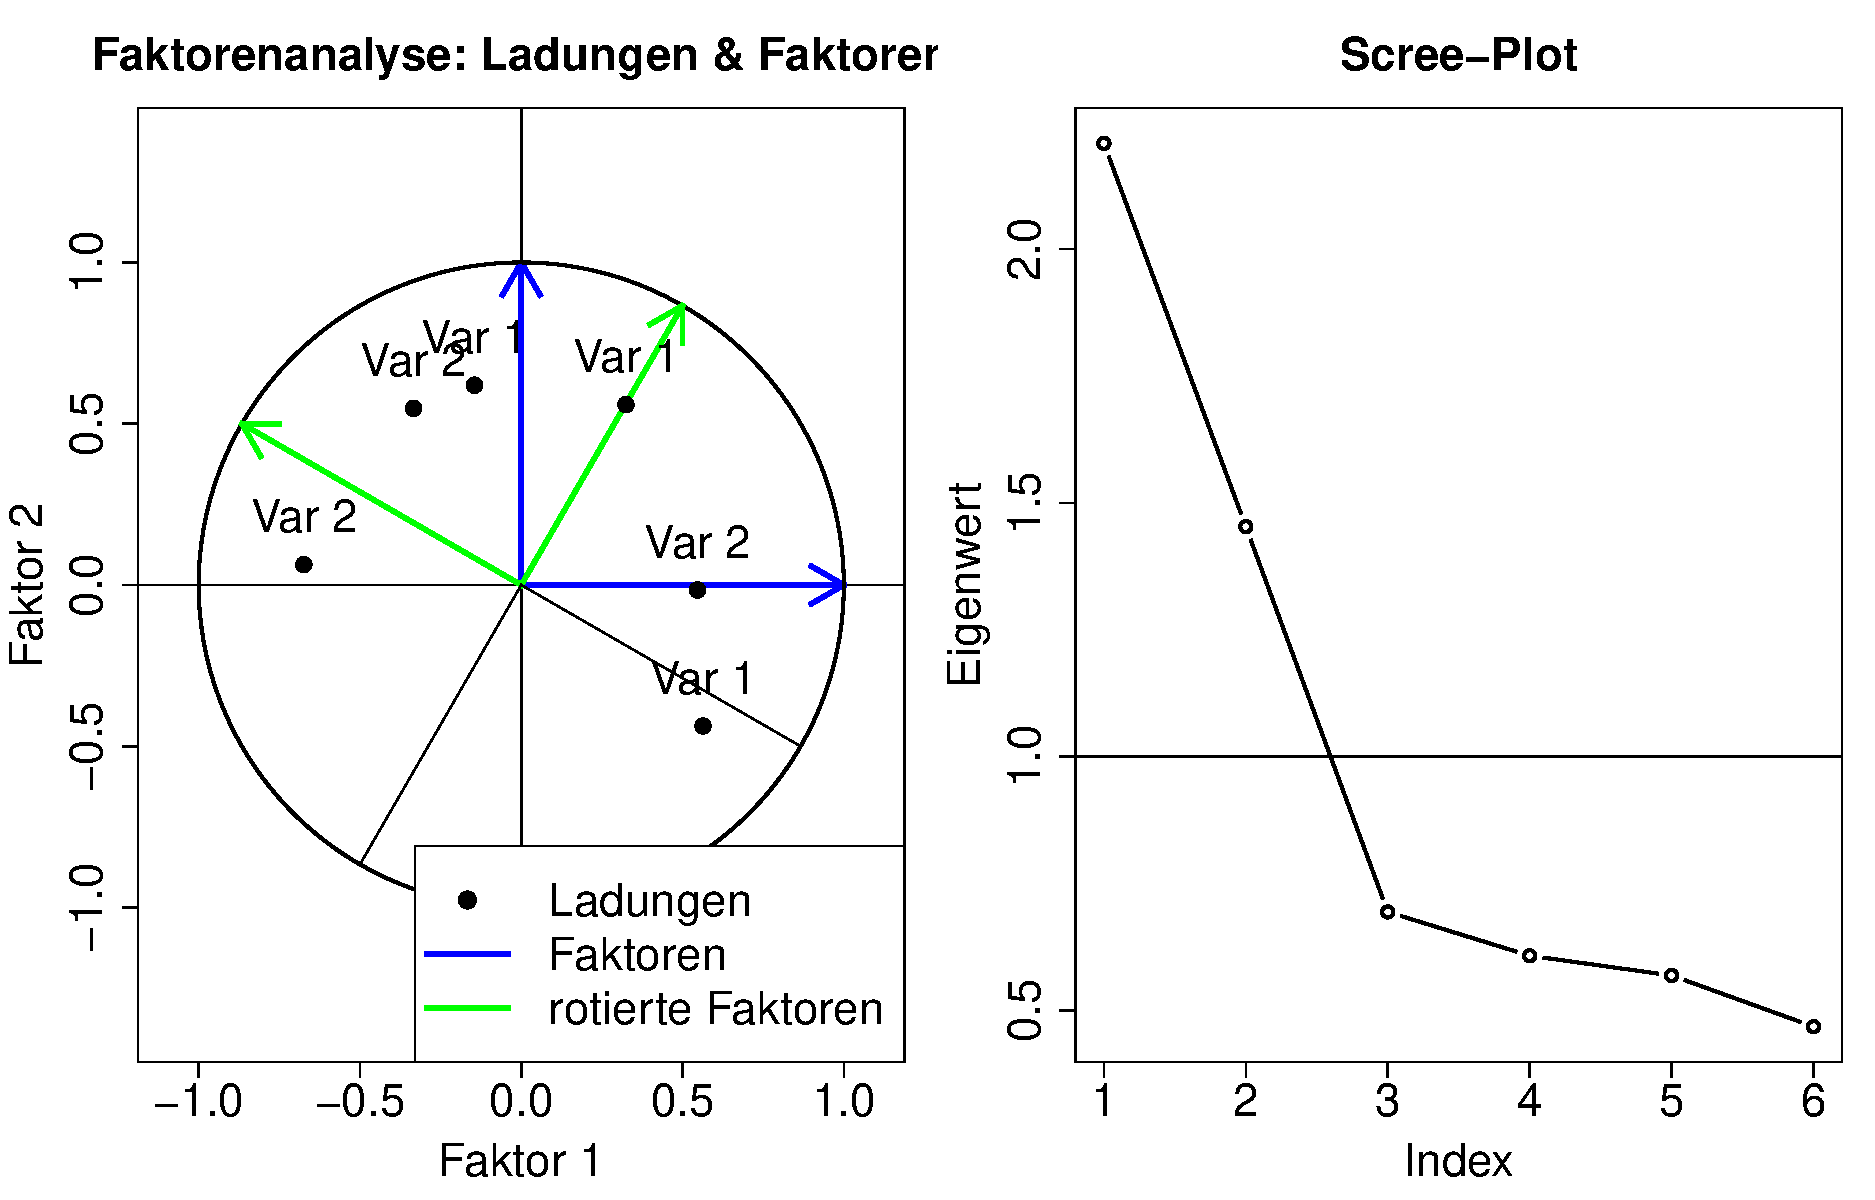
\includegraphics[width=12.5cm]{faLoadings}
\vspace*{-1em}
\caption{Faktorenanalyse: Faktorladungen der Variablen sowie rotierte Faktoren. Scree-Plot der Eigenwerte der Korrelationsmatrix der Daten}
\label{fig:fa}
\end{figure}

Durch orthogonale oder schiefwinklige Rotation der Faktoren lassen sich aus der von \lstinline!factanal()! geschätzten Ladungsmatrix und den zugehörigen Faktorwerten weitere Ladungsmatrizen berechnen, die eine ebenso gute Reproduktion der beobachteten Korrelationsmatrix $\bm{K}_{\bm{x}}$ liefern. Ist allgemein die Rotationsmatrix $\bm{G}$ eine Orthogonalmatrix ($\bm{G}^{\top} = \bm{G}^{-1}$), ergibt sich die neue geschätzte Ladungsmatrix $\tilde{\bm{\Lambda}}$ im Modell unkorrelierter Faktoren aus der alten durch $\tilde{\bm{\Lambda}} = \hat{\bm{\Lambda}} \bm{G}$ (Abb.\ \ref{fig:fa}). Die neue geschätzte Korrelationsmatrix $\tilde{\bm{\Lambda}} \tilde{\bm{\Lambda}}^{\top} + \hat{\bm{D}}_{\bm{\epsilon}}$ stimmt dann mit $\hat{\bm{\Lambda}} \hat{\bm{\Lambda}}^{\top} + \hat{\bm{D}}_{\bm{\epsilon}}$ überein.
\begin{lstlisting}
> ang <- pi/3                     # Rotationswinkel

# Matrix für orthogonale Rotation der Faktoren
> G <- matrix(c(cos(ang), sin(ang), -sin(ang), cos(ang)), nrow=2)
> (Lrot <- Lhat %*% G)            # neue Ladungsmatrix
            [,1]          [,2]
[1,] -0.09662051  -0.706502158
[2,]  0.25977831  -0.480731207
[3,]  0.46393903   0.435109654
[4,]  0.30755796   0.562791872
[5,]  0.64659330  -0.001618208
[6,] -0.28224873   0.615199187

# neue geschätzte Korrelationsmatrix der beobachtbaren Variablen
> KxEstRot <- Lrot %*% t(Lrot) + diag(fa$uniquenesses)
> all.equal(KxEst, KxEstRot)      # Kontrolle: stimmt mit alter überein
[1] TRUE

# rotierte Faktoren einzeichnen
> arrows(0, 0, G[1, ], G[2, ], col="green", lwd=2)
> segments(0, 0, -G[1, ], -G[2, ])

# Variablen beschriften und Legende einfügen
> text(Lhat[ , 1], Lhat[ , 2]+0.06, labels=paste("Var", 1:Q))
> legend(x="bottomright", legend=c("Ladungen", "Faktoren",
+        "rotierte Faktoren"), pch=c(20, NA, NA),
+        lty=c(NA, 1, 1), col=c("black", "blue", "green"))

# Scree-Plot der Eigenwerte der Korrelationsmatrix der Daten
> plot(eigen(cor(X))$values, type="b", ylab="Eigenwert",
+      main="Scree-Plot")

> abline(h=1)                   # Referenzlinie für Kaiser-Kriterium
\end{lstlisting}

Ist $\bm{G}$ eine schiefwinklige Rotationsmatrix, ergibt sich die neue geschätzte Ladungsmatrix $\tilde{\bm{\Lambda}}$ aus der alten durch $\tilde{\bm{\Lambda}} = \hat{\bm{\Lambda}} (\bm{G}^{\top})^{-1}$. Die neue geschätzte Korrelationsmatrix der Faktoren ist $\tilde{\bm{K}}_{\bm{f}} = \bm{G}^{\top} \hat{\bm{K}}_{\bm{f}} \bm{G}$. Die geschätzte Faktorstruktur, also die Matrix der Korrelationen zwischen beobachtbaren Variablen und Faktoren, berechnet sich hier als $\hat{\bm{\Lambda}} \hat{\bm{K}}_{\bm{f}} \bm{G}$. Die neue geschätzte Korrelationsmatrix $\tilde{\bm{\Lambda}} \tilde{\bm{K}}_{\bm{f}} \tilde{\bm{\Lambda}}^{\top} + \hat{\bm{D}}_{\bm{\epsilon}}$ stimmt dann mit $\hat{\bm{\Lambda}} \hat{\bm{K}}_{\bm{f}} \hat{\bm{\Lambda}}^{\top} + \hat{\bm{D}}_{\bm{\epsilon}}$ überein.
\begin{lstlisting}
# Matrix für schiefwinklige Rotation der Faktoren
> G <- matrix(c(0.7071, 0.7071, -0.866, 0.5), nrow=2)

# neue Korrelationsmatrix der Faktoren (bisher: Einheitsmatrix)
> KfRot <- t(G) %*% diag(Q) %*% G

# neue geschätzte Ladungsmatrix
> Lrot <- Lhat %*% solve(t(G))

# neue geschätzte Faktorstruktur
> facStruct <- Lhat %*% diag(Q) %*% G

# neue geschätzte Korrelationsmatrix der beobachtbaren Variablen
> KxEstRot <- Lrot %*% KfRot %*% t(Lrot) + diag(fa$uniquenesses)
> all.equal(KxEst, KxEstRot)    # Kontrolle: stimmt mit alter überein
[1] TRUE
\end{lstlisting}

%%%%%%%%%%%%%%%%%%%%%%%%%%%%%%%%%%%%%%%%%%%%%%%%%%%%%%%%%%%%%%%%%%
%%%%%%%%%%%%%%%%%%%%%%%%%%%%%%%%%%%%%%%%%%%%%%%%%%%%%%%%%%%%%%%%%%
\section{Multidimensionale Skalierung}
\label{sec:multMDS}
%%%%%%%%%%%%%%%%%%%%%%%%%%%%%%%%%%%%%%%%%%%%%%%%%%%%%%%%%%%%%%%%%%
%%%%%%%%%%%%%%%%%%%%%%%%%%%%%%%%%%%%%%%%%%%%%%%%%%%%%%%%%%%%%%%%%%

\index{multidimensionale Skalierung}
Die multidimensionale Skalierung ist ein weiteres Verfahren zur Dimensionsreduktion mit dem Ziel, Beobachtungsobjekte in einem Raum so anzuordnen, dass ihre räumliche Lage zueinander jeweils ihre globale paarweise Unähnlichkeit widerspiegelt. Der Raum soll von möglichst wenigen Merkmalsdimensionen aufgespannt sein. Eine gewählte Anordnung wird als \emph{Konfiguration} bezeichnet. Die inhaltliche Bedeutung der resultierenden Merkmalsdimensionen muss aus den Ergebnissen indirekt erschlossen werden.

Die Ausgangssituation unterscheidet sich von jener in der Hauptkomponentenanalyse\footnote{Tatsächlich sind beide Verfahren eng verwandt, s.\ Abschn.\ \ref{sec:pcaCalc}, Fußnote \ref{ftn:pcamds} sowie Abschn.\ \ref{sec:pcaDimReduce}.} und der Faktorenanalyse dahingehend, dass zunächst unbekannt ist, bzgl.\ welcher Merkmale Objekte beurteilt werden, wenn eine Aussage über ihre generelle Ähnlichkeit zu anderen Objekten getroffen wird. Anders formuliert sind Anzahl und Bedeutung der Variablen, für die Objekte Werte besitzen, nicht gegeben. Dementsprechend werden in einer empirischen Erhebung oft auch nicht separat bestimmte Eigenschaften von einzelnen Objekten gemessen -- vielmehr gilt es, in einem Paarvergleich das Ausmaß der Unähnlichkeit von je zwei Objekte zu beurteilen.

Die \emph{metrische} multidimensionale Skalierung sucht nach einer Konfiguration, so dass die paarweise Unähnlichkeit möglichst gut mit dem jeweiligen euklidischen Abstand zwischen den Punkten übereinstimmt.\footnote{Andere Metriken als der euklidische Abstand sind auch möglich. Die nichtmetrische multidimensionale Skalierung wird durch \lstinline!monoMDS()!\index[func]{monoMDS()@\lstinline{monoMDS()}} aus dem \lstinline!vegan!\index[pack]{vegan@\lstinline{vegan}} Paket \cite{Oksanen2011} bereit gestellt.} Sie wird mit \lstinline!cmdscale()!\index[func]{cmdscale()@\lstinline{cmdscale()}} durchgeführt.
\begin{lstlisting}
cmdscale(d=<<Distanzmatrix>>, k=<<Anzahl an Dimensionen>>, x.ret=FALSE)
\end{lstlisting}

Als Argument \lstinline!d! ist eine symmetrische Matrix zu übergeben, deren Zeilen und Spalten dieselben Objekte repräsentieren. Die Abstände zwischen verschiedenen Objekten i.\,S.\ von Werten eines Unähnlichkeitsmaßes sind in den Zellen außerhalb der Hauptdiagonale enthalten, die selbst überall $0$ ist. Liegen als Daten nicht bereits die Abstände zwischen Objekten vor, sondern die separat für alle Objekte erhobenen Werte bzgl.\ derselben Variablen, können diese mit \lstinline!dist()! in eine geeignete Distanzmatrix transformiert werden (Abschn.\ \ref{sec:matNorm}). Für \lstinline!k! ist anzugeben, durch wie viele Variablen der Raum aufgespannt werden soll, in dem \lstinline!cmdscale()! die Objekte anordnet und ihre euklidischen Distanzen berechnet. Liegen Unähnlichkeitswerte zwischen $n$ Objekten vor, kann die gewünschte Dimension höchstens $n-1$ sein, Voreinstellung ist $2$.

Die Ausgabe umfasst eine $(n \times k)$-Matrix mit den $n$ Koordinaten der Objekte im $k$-dimensionalen Variablenraum, wobei das Zentroid im Ursprung des Koordinatensystems liegt. Mit \lstinline!x.ret=TRUE! enthält das Ergebnis zwei zusätzliche Informationen: die Matrix der paarweisen Distanzen der Objekte bzgl.\ der ermittelten Merkmalsdimensionen und ein Maß für die Güte der Anpassung der ursprünglichen Unähnlichkeiten durch die euklidischen Distanzen. Das Ergebnis ist insofern uneindeutig, als Rotation, Spiegelung und gleichförmige Verschiebung der Punkte ihre Distanzen zueinander nicht ändern.

Als Beispiel liegen die Straßen-Entfernungen zwischen deutschen Städten vor, die die multidimensionale Skalierung auf zwei Dimensionen räumlich anordnen soll.
\begin{lstlisting}
# Städte, deren Entfernungen berücksichtigt werden
> cities <- c("Augsburg", "Berlin", "Dresden", "Hamburg", "Hannover",
+             "Karlsruhe", "Kiel", "München", "Rostock", "Stuttgart")

# erstelle Distanzmatrix aus Vektor der Entfernungen
> n       <- length(cities)                   # Anzahl der Städte
> dstMat  <- matrix(numeric(n^2), nrow=n)     # zunächst leere Matrix
> cityDst <- c(596, 467, 743, 599, 226, 838,  65, 782, 160,
+              194, 288, 286, 673, 353, 585, 231, 633, 477,
+              367, 550, 542, 465, 420, 510, 157, 623,  96,
+              775, 187, 665, 480, 247, 632, 330, 512, 723,
+              298, 805,  80, 872, 206, 752, 777, 220, 824)

> dstMat[upper.tri(dstMat)] <- rev(cityDst)
> dstMat <- t(dstMat[ , n:1])[ , n:1]
> dstMat[lower.tri(dstMat)] <- t(dstMat)[lower.tri(dstMat)]

# füge Städtenamen in Zeilen und Spalten hinzu
> dimnames(dstMat) <- list(city=cities, city=cities)
> (mds <- cmdscale(dstMat, k=2))        # multidimensionale Skalierung
                [,1]        [,2]
Augsburg   399.60802   -70.51443
Berlin    -200.20462  -183.39465
Dresden    -18.47337  -213.01950
Hamburg   -316.39991   130.72245
Hannover  -161.38209   120.21761
Karlsruhe  333.38724   212.12523
Kiel      -409.08703   147.62226
München    408.55752  -144.46446
Rostock   -401.19605  -126.20651
Stuttgart  365.19030   126.91200
\end{lstlisting}

Eine grafische Darstellung der ermittelten Koordinaten erlaubt es, das Ergebnis mit den tatsächlichen Positionen zu vergleichen (Abb.\ \ref{fig:mds}). Hier ist zu erkennen, dass das Ergebnis für die meisten Städte gut mit der realen Topografie übereinstimmt, wenn man die Möglichkeit einer Drehung im Uhrzeigersinn um $90^{\circ}$ berücksichtigt und dann die West-Ost-Richtung spiegelt.
\begin{lstlisting}
> xLims <- range(mds[ , 1]) + c(0, 250)       # x-Achsenbereich
> plot(mds, xlim=xLims, xlab="Nord-Süd", ylab="Ost-West", pch=16,
+      main="Anordnung der Städte nach MDS")

# füge Städtenamen hinzu
> text(mds[ , 1]+50, mds[ , 2], adj=0, labels=cities)
\end{lstlisting}

\begin{figure}[ht]
\centering
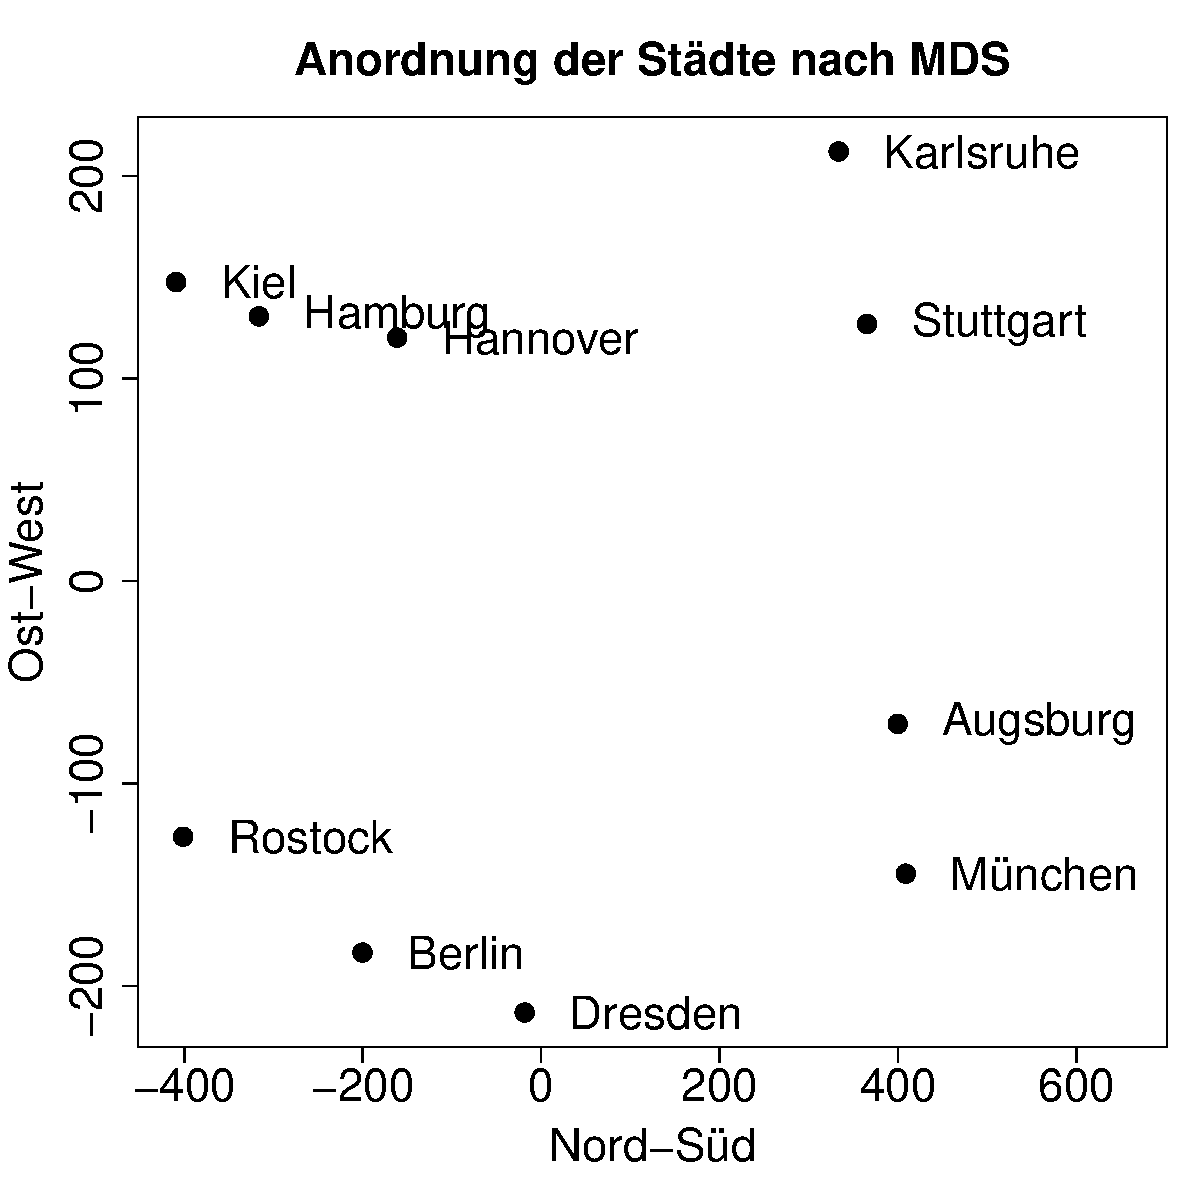
\includegraphics[width=8cm]{mds}
\vspace*{-1em}
\caption{Ergebnis der multidimensionalen Skalierung auf Basis der Distanzen zwischen deutschen Städten}
\label{fig:mds}
\end{figure}

%%%%%%%%%%%%%%%%%%%%%%%%%%%%%%%%%%%%%%%%%%%%%%%%%%%%%%%%%%%%%%%%%%
%%%%%%%%%%%%%%%%%%%%%%%%%%%%%%%%%%%%%%%%%%%%%%%%%%%%%%%%%%%%%%%%%%
\section{Multivariate multiple Regression}
\label{sec:multRegrMult}
%%%%%%%%%%%%%%%%%%%%%%%%%%%%%%%%%%%%%%%%%%%%%%%%%%%%%%%%%%%%%%%%%%
%%%%%%%%%%%%%%%%%%%%%%%%%%%%%%%%%%%%%%%%%%%%%%%%%%%%%%%%%%%%%%%%%%

\index{Regression!multivariate|textbf}
Die univariate multiple Regression (Abschn.\ \ref{sec:regrMult}) lässt sich zur multivariaten multiplen Regression verallgemeinern, bei der durch $p$ Prädiktoren $X_{j}$ (mit $j = 1, \ldots, p$) nicht nur ein Kriterium $Y$ vorhergesagt werden soll, sondern $r$ Kriteriumsvariablen $Y_{l}$ (mit $l = 1, \ldots, r$) gleichzeitig. Die Parameterschätzung im multivariaten Fall ist auf den univariaten zurückführbar: Die i.\,S.\ der geringsten Quadratsumme der Residuen optimale Parameterwahl geht aus der Zusammenstellung der $r$ unabhängig voneinander durchgeführten Regressionen von jeweils einem Kriterium $Y_{l}$ auf alle Prädiktoren $X_{j}$ hervor.

In der Berechnung der multivariaten multiplen Regression mittels \lstinline!lm()!\index[func]{lm()@\lstinline{lm()}} ist die Modellformel zunächst wie im univariaten Fall aufzubauen. Im Unterschied dazu ist das Kriterium auf der linken Seite der Formel hier jedoch kein Vektor, sondern muss eine spaltenweise aus den einzelnen Kriteriumsvariablen zusammengestellte Matrix sein.

Im Beispiel sollen anhand der Prädiktoren Alter, Körpergröße und wöchentliche Dauer sportlicher Aktivitäten die Kriterien Körpergewicht und Gesundheit (i.\,S.\ eines geeigneten quantitativen Maßes) vorhergesagt werden.
\begin{lstlisting}
> N      <- 100                          # Anzahl Versuchspersonen
> height <- rnorm(N, 175, 7)             # Prädiktor 1
> age    <- rnorm(N, 30, 8)              # Prädiktor 2
> sport  <- abs(rnorm(N, 60, 30))        # Prädiktor 3

# modellgerechte Simulation beider Kriterien
> weight <- 0.5*height - 0.3*age - 0.4*sport + 10 + rnorm(N, 0, 3)
> health <- -0.3*age + 0.6*sport + rnorm(N, 4)
> Y      <- cbind(weight, health)        # Matrix der Kriterien

# multivariat formulierte Modellformel für lm()
> (fitM <- lm(Y ~ height + age + sport))
Call:
lm(formula = Y ~ height + age + sport)

Coefficients:
              weight    health
(Intercept) 10.41235   2.44980
height       0.50721   0.01031
age         -0.34730  -0.29678
sport       -0.40894   0.59826

# Kontrolle: Koeffizienten beider univariater Regressionen separat
> coef(lm(weight ~ height + age + sport))
(Intercept)  height      age    sport
    10.4124  0.5072  -0.3473  -0.4089

> coef(lm(health ~ height + age + sport))
Coefficients:
(Intercept)   height       age    sport
   2.44980   0.01031  -0.29678  0.59826
\end{lstlisting}

Die multivariate Regressionsanalyse als inferenzstatistischer Test liefert i.\,d.\,R.\ andere Ergebnisse als die separaten univariaten Regressionsanalysen (Abschn.\ \ref{sec:multALMmodCmp}, \ref{sec:multALMtest}). Das von \lstinline!lm()! erzeugte Objekt muss dazu an die Funktion \lstinline!summary(manova())!\index[func]{manova()@\lstinline{manova()}|textbf} übergeben werden, die \lstinline!aov()! (Abschn.\ \ref{sec:aov}) auf den multivariaten Fall verallgemeinert und ebenso wie diese aufzurufen ist. Mit dem Argument \lstinline!test! von \lstinline!summary()! lassen sich verschiedene multivariate Teststatistiken wählen, etwa die Hotelling-Lawley-Spur mit \lstinline!"Hotelling-Lawley"! (für weitere vgl.\ \lstinline!?summary.manova! und Abschn.\ \ref{sec:multALMtest}). Anders als bei den univariaten Tests ist beim multivariaten Test der Parameter die Reihenfolge der Prädiktoren relevant (für die manuelle Kontrolle s.\ Abschn.\ \ref{sec:multALMexRegr}).
\begin{lstlisting}
> summary(manova(fitM), test="Hotelling-Lawley")
          Df Hotelling-Lawley approx F num Df den Df    Pr(>F)
height     1            8.056    382.7      2     95 < 2.2e-16 ***
age        1            6.897    327.6      2     95 < 2.2e-16 ***
sport      1          257.924  12251.4      2     95 < 2.2e-16 ***
Residuals 96
\end{lstlisting}

%%%%%%%%%%%%%%%%%%%%%%%%%%%%%%%%%%%%%%%%%%%%%%%%%%%%%%%%%%%%%%%%%%
%%%%%%%%%%%%%%%%%%%%%%%%%%%%%%%%%%%%%%%%%%%%%%%%%%%%%%%%%%%%%%%%%%
\section[Hotellings \texorpdfstring{$T^{2}$}{T2}]{Hotellings \texorpdfstring{$\bm{T^{2}}$}{T2}}
\label{sec:multHotelling}
%%%%%%%%%%%%%%%%%%%%%%%%%%%%%%%%%%%%%%%%%%%%%%%%%%%%%%%%%%%%%%%%%%
%%%%%%%%%%%%%%%%%%%%%%%%%%%%%%%%%%%%%%%%%%%%%%%%%%%%%%%%%%%%%%%%%%

%%%%%%%%%%%%%%%%%%%%%%%%%%%%%%%%%%%%%%%%%%%%%%%%%%%%%%%%%%%%%%%%%%
%%%%%%%%%%%%%%%%%%%%%%%%%%%%%%%%%%%%%%%%%%%%%%%%%%%%%%%%%%%%%%%%%%
\subsection{Test für eine Stichprobe}
\label{sec:multHotellingOne}
%%%%%%%%%%%%%%%%%%%%%%%%%%%%%%%%%%%%%%%%%%%%%%%%%%%%%%%%%%%%%%%%%%
%%%%%%%%%%%%%%%%%%%%%%%%%%%%%%%%%%%%%%%%%%%%%%%%%%%%%%%%%%%%%%%%%%

\index{Hotellings T2@Hotellings $T^{2}$!eine Stichprobe}
Hotellings $T^{2}$-Test für eine Stichprobe prüft die Datenvektoren von $r$ gemeinsam normalverteilten Variablen daraufhin, ob sie mit der $\text{H}_{0}$ konsistent sind, dass ihr theoretisches Zentroid $\bm{\mu}$ mit einem bestimmten Vektor $\bm{\mu}_{0}$ übereinstimmt. Der zweiseitige univariate $t$-Test (Abschn.\ \ref{sec:tOne}) ist zu Hotellings $T^{2}$-Test äquivalent, wenn nur Daten einer Zielgröße vorliegen. Der Test lässt sich mit der aus der univariaten Varianzanalyse (Abschn.\ \ref{sec:anova}) bekannten Funktion\index[func]{anova()@\lstinline{anova()}}\index[func]{lm()@\lstinline{lm()}}
\begin{lstlisting}
anova(lm(<<AV>> ~ 1, data=<<Datensatz>>), test="Hotelling-Lawley")
\end{lstlisting}

durchführen. In der für \lstinline!lm()! anzugebenden Formel \lstinline!<<AV>> ~ 1! sind die \lstinline!<<AV>>! Werte dabei multivariat, d.\,h. in Form einer spaltenweise aus den einzelnen Variablen zusammengestellten Matrix zu übergeben. Von den Zeilenvektoren der Daten muss zunächst das Zentroid unter $\text{H}_{0}$ abgezogen werden, damit die Formel zum Test der $\text{H}_{0}: \bm{\mu} - \bm{\mu}_{0} = \bm{0}$ führt, die äquivalent zu $\bm{\mu} = \bm{\mu}_{0}$ ist. Stammen die Variablen aus einem Datensatz, ist dieser unter \lstinline!data! zu nennen. Weiter ist das Argument \lstinline!test! von \lstinline!anova()! zu verwenden, um eine multivariate Teststatistik auszuwählen.\footnote{Bei der multivariaten Formulierung des Modells wird intern aufgrund der generischen \lstinline!anova()! Funktion automatisch \lstinline!anova.mlm()! verwendet, ohne dass dies explizit angegeben werden muss (Abschn.\ \ref{sec:funcGeneric}).} Dies kann \lstinline!"Hotelling-Lawley"! für die Hotelling-Lawley-Spur sein, wobei die Wahl hier nicht relevant ist: Wenn nur eine Bedingung vorliegt, sind alle auswählbaren Teststatistiken zu Hotellings $T^{2}$-Statistik äquivalent.

Im Beispiel sollen die Werte zweier Variablen betrachtet werden. Zunächst sind nur die Daten aus einer Stichprobe (von später dreien) relevant.
\begin{lstlisting}
> muH0 <- c(-3, 2)                        # Zentroid unter H0
     
# theoretische 2x2 Kovarianzmatrix für Zufallsvektoren
> sigma <- matrix(c(16,-2, -2,9), byrow=TRUE, ncol=2)
> mu11  <- c(-4, 4)                       # theoretisches Zentroid
> Nj    <- c(15, 25, 20)                  # Gruppengrößen

# Datenmatrix für 1. Gruppe mit Variablen in den Spalten
> library(mvtnorm)                        # für rmvnorm()
> Y11  <- round(rmvnorm(Nj[1], mean=mu11, sigma=sigma))

# ziehe Zentroid unter H0 von allen Zeilenvektoren ab
> Y11ctr <- scale(Y11, center=muH0, scale=FALSE)
> (anRes <- anova(lm(Y11ctr ~ 1), test="Hotelling-Lawley"))
            Df Hotelling-Lawley approx F num Df den Df   Pr(>F)
(Intercept)  1           1.3987   9.0917      2     13 0.003390 **
Residuals   14
\end{lstlisting}

Die Ausgabe nennt die Hotelling-Lawley-Spur $\text{tr}_{\text{HL}}$ in der Spalte \lstinline!Hotelling-Lawley!, die $F$-verteilte Teststatistik $\frac{n-r}{r} \text{tr}_{\text{HL}}$ in der Spalte \lstinline!approx F!. Weiterhin sind die Freiheitsgrade der zugehörigen F-Verteilung (\lstinline!num Df!, \lstinline!den Df!) und der entsprechende $p$-Wert (\lstinline!Pr(>F)!) aufgeführt.

Das Ergebnis lässt sich auch manuell prüfen. Hotellings $T^{2}$ ist gleich dem $n$-fachen der quadrierten Mahalanobisdistanz zwischen dem Zentroid der Daten und dem Zentroid unter $\text{H}_{0}$ bzgl.\ der korrigierten Kovarianzmatrix der Daten (Abschn.\ \ref{sec:mahaDist}). Außerdem gilt $T^{2} = (n-1) \text{tr}_{\text{HL}}$.
\begin{lstlisting}
> n   <- nrow(Y11)                            # Stichprobengröße
> ctr <- colMeans(Y11)                        # Zentroid

# Hotellings T^2 Teststatistik
> (T2 <- n * (t(ctr-muH0) %*% solve(cov(Y11)) %*% (ctr-muH0)))
[1,] 19.58203

# Kontrolle: n-faches der quadrierten Mahalanobisdistanz
> n * mahalanobis(ctr, muH0, cov(Y11))
[1] 19.58203

# Hotelling-Lawley-Spur
> Tr_HL <- anRes[1, "Hotelling-Lawley"]
> (n-1) * Tr_HL
[1] 19.58203

> r     <- ncol(Y11)                          # Anzahl Variablen
> (F_HL <- ((n-r) / r) * Tr_HL)               # Teststatistik
[1] 9.091655

> (pVal <- pf(F_HL, r, n-r, lower.tail=FALSE))     # p-Wert
[1] 0.003389513
\end{lstlisting}

%%%%%%%%%%%%%%%%%%%%%%%%%%%%%%%%%%%%%%%%%%%%%%%%%%%%%%%%%%%%%%%%%%
%%%%%%%%%%%%%%%%%%%%%%%%%%%%%%%%%%%%%%%%%%%%%%%%%%%%%%%%%%%%%%%%%%
\subsection{Test für zwei unabhängige Stichproben}
\label{sec:multHotellingTwoInd}
%%%%%%%%%%%%%%%%%%%%%%%%%%%%%%%%%%%%%%%%%%%%%%%%%%%%%%%%%%%%%%%%%%
%%%%%%%%%%%%%%%%%%%%%%%%%%%%%%%%%%%%%%%%%%%%%%%%%%%%%%%%%%%%%%%%%%

\index{Hotellings T2@Hotellings $T^{2}$!zwei unabhängige Stichproben}
Hotellings $T^{2}$-Test für zwei unabhängige Stichproben prüft die in zwei Bedingungen erhobenen Datenvektoren von $r$ gemeinsam normalverteilten Variablen mit identischen Kovarianzmatrizen daraufhin, ob sie mit der $\text{H}_{0}$ konsistent sind, dass ihre theoretischen Zentroide übereinstimmen. Der Test ist äquivalent zum univariaten $t$-Test für zwei unabhängige Stichproben, wenn nur Werte einer Zielgröße vorliegen (Abschn.\ \ref{sec:tTwoInd}).

Hotellings $T^{2}$-Test lässt sich wie der Test für eine Stichprobe in Abschn.\ \ref{sec:multHotellingOne} durchführen. Dabei sind in der Modellformel \lstinline!<<AV>> ~ <<UV>>! für \lstinline!lm()! die \lstinline!<<AV>>! Werte beider Gruppen in Form einer spaltenweise aus den einzelnen Variablen zusammengestellten Matrix zu nennen, deren Zeilen von den Beobachtungsobjekten gebildet werden. \lstinline!<<UV>>! codiert in Form eines Faktors für jede Zeile der \lstinline!<<AV>>! Matrix, aus welcher Bedingung der zugehörige Datenvektor stammt. Das Argument \lstinline!test! von \lstinline!anova()! kann auf \lstinline!"Hotelling-Lawley"! für die Hotelling-Lawley-Spur gesetzt werden, wobei auch bei zwei Gruppen alle multivariaten Teststatistiken äquivalent sind.

Das im vorangehenden Abschnitt begonnene Beispiel soll nun um die in einer zweiten Bedingung erhobenen Daten der betrachteten Variablen erweitert werden. Als Teststatistik wird hier wieder die Hotelling-Lawley-Spur $\text{tr}_{\text{HL}}$ gewählt.
\begin{lstlisting}
> mu21 <- c(3, 3)               # Zentroid Zufallsvektoren 2. Bedingung

# Datenmatrix aus 2. Bedingung mit Variablen in den Spalten
> library(mvtnorm)              # für rmvnorm()
> Y21 <- round(rmvnorm(Nj[2], mean=mu21, sigma=sigma))
> Yht <- rbind(Y11, Y21)        # Gesamt-Datenmatrix beider Bedingungen

# codiere für jede Zeile der Datenmatrix die zugehörige Bedingung
> IVht <- factor(rep(1:2, Nj[1:2]))
> anova(lm(Yht ~ IVht), test="Hotelling-Lawley")
Analysis of Variance Table
            Df Hotelling-Lawley approx F num Df den Df    Pr(>F)
(Intercept)  1           2.4627   45.560      2     37 1.049e-10 ***
IVht         1           0.6073   11.235      2     37 0.0001539 ***
Residuals   38
\end{lstlisting}

Die Ausgabe ist analog zu Abschn.\ \ref{sec:multHotellingOne}, die Kennwerte des Tests des Faktors stehen in der mit seinem Namen bezeichneten Zeile. Für die Teststatistik gilt $F = \frac{n_{1} + n_{2}-r-1}{r} \text{tr}_{\text{HL}}$.

Schließlich existiert mit \lstinline!manova()!\index[func]{manova()@\lstinline{manova()}} eine Funktion, die \lstinline!aov()! (Abschn.\ \ref{sec:aov}) auf den multivariaten Fall verallgemeinert und ebenso wie diese aufzurufen ist. Die Modellformel ist dieselbe wie beim Aufruf von \lstinline!lm()!.
\begin{lstlisting}
> (sumRes <- summary(manova(Yht ~ IVht), test="Hotelling-Lawley"))
          Df Hotelling-Lawley approx F num Df den Df    Pr(>F)
IVht       1           0.6073   11.235      2     37 0.0001539 ***
Residuals 38
\end{lstlisting}

Das Ergebnis lässt sich auch manuell prüfen. Hotellings $T^{2}$ ist bis auf einen Faktor gleich der quadrierten Mahalanobisdistanz beider Zentroide bzgl.\ einer geeigneten Schätzung der Kovarianzmatrix der Differenzvektoren. Außerdem gilt $T^{2} = (n_{1}+n_{2}-2) \text{tr}_{\text{HL}}$.
\begin{lstlisting}
> n1   <- nrow(Y11)                         # Gruppengröße 1
> n2   <- nrow(Y21)                         # Gruppengröße 2
> ctr1 <- colMeans(Y11)                     # Zentroid 1. Bedingung
> ctr2 <- colMeans(Y21)                     # Zentroid 2. Bedingung

# unkorrigierte Kovarianzmatrizen aus beiden Bedingungen
> S1 <- cov.wt(Y11, method="ML")$cov
> S2 <- cov.wt(Y21, method="ML")$cov

# mit Stichprobengröße gewichtete Summe der Kovarianzmatrizen
> Su <- (1 / (n1+n2-2)) * (n1*S1 + n2*S2)

# Hotellings T^2
> T2 <- ((n1*n2)/(n1+n2))*(t(ctr2-ctr1) %*% solve(Su) %*% (ctr2-ctr1))
> T2
[1,] 23.07731

# Kontrolle: quadrierte Mahalanobisdistanz beider Zentroide bzgl. Su
> ((n1*n2) / (n1+n2)) * mahalanobis(ctr1, ctr2, Su)
[1] 23.07731

# Hotelling-Lawley-Spur
> Tr_HL <- sumRes$stats["IVht", "Hotelling-Lawley"]

# Kontrolle: T^2 = (n1+n2-2) * Hotelling-Lawley-Spur
> (n1+n2-2) * Tr_HL
[1] 23.07731

> r     <- ncol(Y11)                              # Anzahl Variablen
> (F_HL <- ((n1+n2-r-1) / r) * Tr_HL)             # Teststatistik
[1] 11.23501

> (pVal <- pf(F_HL, r, n1+n2-r-1, lower.tail=FALSE))       # p-Wert
[1] 0.0001538927
\end{lstlisting}

%%%%%%%%%%%%%%%%%%%%%%%%%%%%%%%%%%%%%%%%%%%%%%%%%%%%%%%%%%%%%%%%%%
%%%%%%%%%%%%%%%%%%%%%%%%%%%%%%%%%%%%%%%%%%%%%%%%%%%%%%%%%%%%%%%%%%
\subsection{Test für zwei abhängige Stichproben}
%%%%%%%%%%%%%%%%%%%%%%%%%%%%%%%%%%%%%%%%%%%%%%%%%%%%%%%%%%%%%%%%%%
%%%%%%%%%%%%%%%%%%%%%%%%%%%%%%%%%%%%%%%%%%%%%%%%%%%%%%%%%%%%%%%%%%

\index{Hotellings T2@Hotellings $T^{2}$!zwei abhängige Stichproben}
Analog zum univariaten $t$-Test (Abschn.\ \ref{sec:tTwoDep}) kann der multivariate $T^{2}$-Test für zwei abhängige Stichproben auf die Situation einer Stichprobe zurückgeführt werden: Dazu bildet man variablenweise pro Beobachtungsobjekt die Differenz der Daten aus beiden Bedingungen und stellt die Differenzvariablen spaltenweise zu einer neuen Matrix zusammen. Hotellings $T^{2}$-Test für eine Stichprobe ist mit diesen Differenzdaten dann mit der $\text{H}_{0}$ durchzuführen, dass ihr theoretisches Zentroid $\bm{\mu}_0 = \bm{0}$ ist. Anders als in Abschn.\ \ref{sec:multHotellingOne} entfällt hier wegen $\bm{\mu}_0 = \bm{0}$ die Notwendigkeit, $\bm{\mu}_0$ von den Zeilenvektoren der Datenmatrix der Differenzvariablen abzuziehen, bevor \lstinline!anova()! aufgerufen wird.
\begin{lstlisting}
> N    <- 20                                # Anzahl Personen
> P    <- 2                                 # Anzahl Messzeitpunkte
> Y1t0 <- rnorm(N, mean=90,  sd=15)         # AV 1 Zeitpunkt t0
> Y1t1 <- rnorm(N, mean=100, sd=15)         # AV 1 Zeitpunkt t1
> Y2t0 <- rnorm(N, mean=85,  sd=15)         # AV 2 Zeitpunkt t0
> Y2t1 <- rnorm(N, mean=105, sd=15)         # AV 2 Zeitpunkt t1

# Faktor, der im Long-Format den Messzeitpunkt codiert
> IV <- factor(rep(1:P, each=N), labels=c("t0", "t1"))
> id <- factor(rep(1:N, times=P))           # Faktor Personen-ID

# Datensatz im Long-Format
> Ydf <- data.frame(id, Y1=c(Y1t0, Y1t1), Y2=c(Y2t0, Y2t1), IV)

# bilde pro Variable personenweise Differenz zwischen t0 und t1
> dfDiff <- aggregate(cbind(Y1, Y2) ~ id, data=Ydf, FUN=diff)
> DVdiff <- data.matrix(dfDiff[ , -1])      # als Matrix
> anova(lm(DVdiff ~ 1), test="Hotelling-Lawley")
Analysis of Variance Table
            Df Hotelling-Lawley approx F num Df den Df   Pr(>F)
(Intercept)  1          0.87529   7.8777      2     18 0.003486 **
Residuals   19
\end{lstlisting}

%%%%%%%%%%%%%%%%%%%%%%%%%%%%%%%%%%%%%%%%%%%%%%%%%%%%%%%%%%%%%%%%%%
%%%%%%%%%%%%%%%%%%%%%%%%%%%%%%%%%%%%%%%%%%%%%%%%%%%%%%%%%%%%%%%%%%
\subsection[Univariate Varianzanalyse mit abhängigen Gruppen (RB-\texorpdfstring{$p$}{p})]{Univariate Varianzanalyse mit abhängigen Gruppen (RB-$\bm{p}$)}
\label{sec:multRBp}
%%%%%%%%%%%%%%%%%%%%%%%%%%%%%%%%%%%%%%%%%%%%%%%%%%%%%%%%%%%%%%%%%%
%%%%%%%%%%%%%%%%%%%%%%%%%%%%%%%%%%%%%%%%%%%%%%%%%%%%%%%%%%%%%%%%%%

\index{Varianzanalyse!einfaktorielle!abhängige Gruppen (RB-$p$)}
Daten einer eigentlich univariaten Varianzanalyse mit $p$ abhängigen Gruppen (RB-$p$ Design, Abschn.\ \ref{sec:RBp}) können auch multivariat ausgewertet werden, wodurch die Voraussetzung der Zirkularität entfällt. Hierfür sind zunächst blockweise alle ${p \choose 2} = \frac{p (p-1)}{2}$ Differenzvariablen zwischen je zwei Gruppen zu bilden und spaltenweise zu einer Matrix zusammenzufassen. Deren Spalten sind für $p > 2$ jedoch linear abhängig, da es höchstens $p-1$ linear unabhängige Differenzvariablen gibt. Um diese Redundanz zu beseitigen, müssen $p-1$ Spalten der Matrix ausgewählt werden, in deren Differenzen insgesamt alle $p$ Gruppen eingeflossen sind. Die übrigen Spalten der ursprünglichen Matrix der Differenzvariablen werden gestrichen. Für die beibehaltenen Differenzvariablen ist Hotellings $T^{2}$-Test für eine Stichprobe mit der $\text{H}_{0}$ durchzuführen, dass ihr Zentroid der Vektor $\bm{0}$ ist. Das Vorgehen ist damit analog zu jenem bei Hotellings $T^{2}$-Test für zwei abhängige Stichproben.

Als Beispiel diene jenes aus Abschn.\ \ref{sec:RBp} mit einer zu vier Messzeitpunkten erhobenen Zielgröße.
\begin{lstlisting}
> P   <- 4                                    # Anzahl Messzeitpunkte
> DVw <- cbind(DV_t1, DV_t2, DV_t3, DV_t4)    # Datenmatrix Wide-Format

# alle paarweisen Differenzen der Spalten der Datenmatrix
> diffMat <- combn(1:P, 2, function(x) { DVw[ , x[1]] - DVw[ , x[2]] })

# wähle P-1 Differenzvariablen, die nicht redundant sein dürfen
> DVdiff <- diffMat[ , 1:(P-1), drop=FALSE]
> anova(lm(DVdiff ~ 1), test="Hotelling-Lawley")
Analysis of Variance Table
            Df Hotelling-Lawley approx F num Df den Df Pr(>F)
(Intercept)  1           1.2474   2.9106      3      7 0.1104
Residuals    9
\end{lstlisting}

Alternativ eignet sich die in Abschn.\ \ref{sec:AnovaRBp} vorgestellte Funktion \lstinline!Anova()!\index[func]{Anova()@\lstinline{Anova()}} aus dem \lstinline!car!\index[pack]{car@\lstinline{car}} Paket, für die Daten im Wide-Format benötigt werden. Für den multivariaten Test ist hier bei der Anwendung von \lstinline!summary()! das Argument \lstinline!multivariate=TRUE! zu setzen. Alle ausgegebenen Teststatistiken sind hier äquivalent zum $T^{2}$-Test, weil letztlich ein multivariater Test für nur eine Gruppe vorliegt.
\begin{lstlisting}
> fitRBp   <- lm(DVw ~ 1)                     # Zwischen-Gruppen Design
> intraRBp <- data.frame(IV=gl(P, 1))         # Intra-Gruppen Design
> library(car)                                # für Anova()
> AnovaRBp <- Anova(fitRBp, idata=intraRBp, idesign=~IV)
> summary(AnovaRBp, multivariate=TRUE, univariate=FALSE)      # ...
\end{lstlisting}

%%%%%%%%%%%%%%%%%%%%%%%%%%%%%%%%%%%%%%%%%%%%%%%%%%%%%%%%%%%%%%%%%%
%%%%%%%%%%%%%%%%%%%%%%%%%%%%%%%%%%%%%%%%%%%%%%%%%%%%%%%%%%%%%%%%%%
%\newpage
\section{Multivariate Varianzanalyse (MANOVA)}
\label{sec:multManova}
%%%%%%%%%%%%%%%%%%%%%%%%%%%%%%%%%%%%%%%%%%%%%%%%%%%%%%%%%%%%%%%%%%
%%%%%%%%%%%%%%%%%%%%%%%%%%%%%%%%%%%%%%%%%%%%%%%%%%%%%%%%%%%%%%%%%%

%%%%%%%%%%%%%%%%%%%%%%%%%%%%%%%%%%%%%%%%%%%%%%%%%%%%%%%%%%%%%%%%%%
%%%%%%%%%%%%%%%%%%%%%%%%%%%%%%%%%%%%%%%%%%%%%%%%%%%%%%%%%%%%%%%%%%
\subsection{Einfaktorielle MANOVA}
\label{sec:multManova1}
%%%%%%%%%%%%%%%%%%%%%%%%%%%%%%%%%%%%%%%%%%%%%%%%%%%%%%%%%%%%%%%%%%
%%%%%%%%%%%%%%%%%%%%%%%%%%%%%%%%%%%%%%%%%%%%%%%%%%%%%%%%%%%%%%%%%%

\index{Varianzanalyse!multivariate!einfaktorielle|textbf}
Die einfaktorielle multivariate Varianzanalyse prüft die in mehreren Bedingungen einer Gruppierungsvariable erhobenen Datenvektoren von $r$ gemeinsam normalverteilten Variablen mit identischen Kovarianzmatrizen daraufhin, ob sie mit der $\text{H}_{0}$ konsistent sind, dass ihre theoretischen Zentroide übereinstimmen. Der Test ist äquivalent zur univariaten einfaktoriellen Varianzanalyse, wenn nur die Daten einer Zielgröße vorliegen (Abschn.\ \ref{sec:CRp}).

Zur Durchführung eignet sich wie bei Hotellings $T^{2}$-Test für zwei Stichproben die \lstinline!manova()!\index[func]{manova()@\lstinline{manova()}} Funktion als Verallgemeinerung von \lstinline!aov()!. Dabei ist die Modellformel links der \lstinline!~! multivariat zu formulieren, also eine spaltenweise aus den Variablen zusammengestellte Datenmatrix mit den Beobachtungsobjekten in den Zeilen zu übergeben. Als Gruppierungsvariable auf der rechten Seite der \lstinline!~! ist ein Faktor zu nennen, der für jede Zeile der Datenmatrix codiert, aus welcher Bedingung der Datenvektor stammt.

Im Test der von \lstinline!manova()! durchgeführten Modellanpassung mit \lstinline!summary()!\index[func]{summary()@\lstinline{summary()}} können verschiedene Teststatistiken über das Argument \lstinline!test! gewählt werden: Voreinstellung ist \lstinline!"Pillai"! für die\index{Pillai-Bartlett-Spur} Pillai-Bartlett-Spur, andere Optionen sind \lstinline!"Wilks"! für\index{Wilks' Lambda@Wilks' $\Lambda$} Wilks' $\Lambda$, \lstinline!"Roy"! für Roys Maximalwurzel\index{Roys Maximalwurzel} und\index{Hotelling-Lawley-Spur} \lstinline!"Hotelling-Lawley"! für die Hotelling-Lawley-Spur (Abschn.\ \ref{sec:multALMtest}). Bei zwei Gruppen sind alle Teststatistiken äquivalent.

Das Beispiel aus Abschnitt \ref{sec:multHotellingOne} und \ref{sec:multHotellingTwoInd} soll nun um die in einer dritten Bedingung erhobenen Daten der betrachteten beiden Variablen erweitert werden (für die manuelle Kontrolle s.\ Abschn.\ \ref{sec:multALMexMan1}).
\begin{lstlisting}
> mu31 <- c(1, -1)              # Zentroid Zufallsvektoren 3. Bedingung

# Datenmatrix aus 3. Bedingung mit Variablen in den Spalten
> library(mvtnorm)               # für rmvnorm()
> Y31   <- round(rmvnorm(Nj[3], mean=mu31, sigma=sigma))
> Ym1   <- rbind(Y11, Y21, Y31)  # Matrix der Daten aus allen Gruppen
> IVman <- factor(rep(1:3, Nj))  # Bedingung für jede Zeile Datenmatrix
> manRes1 <- manova(Ym1 ~ IVman) # Anpassung multivar. Varianzanalyse
> summary(manRes1, test="Wilks")            # Wilks' Lambda
           Df    Wilks  approx F  num Df  den Df    Pr(>F)
IVman       2  0.42011    15.199       4     112  5.89e-10 ***
Residuals  57
\end{lstlisting}

%%%%%%%%%%%%%%%%%%%%%%%%%%%%%%%%%%%%%%%%%%%%%%%%%%%%%%%%%%%%%%%%%%
%%%%%%%%%%%%%%%%%%%%%%%%%%%%%%%%%%%%%%%%%%%%%%%%%%%%%%%%%%%%%%%%%%
\subsection{Zweifaktorielle MANOVA}
\label{sec:multManova2}
%%%%%%%%%%%%%%%%%%%%%%%%%%%%%%%%%%%%%%%%%%%%%%%%%%%%%%%%%%%%%%%%%%
%%%%%%%%%%%%%%%%%%%%%%%%%%%%%%%%%%%%%%%%%%%%%%%%%%%%%%%%%%%%%%%%%%

\index{Varianzanalyse!multivariate!zweifaktorielle|textbf}
Die zweifaktorielle multivariate Varianzanalyse ist wie die einfaktorielle mit \lstinline!manova()!\index[func]{manova()@\lstinline{manova()}} durchzuführen, lediglich die Spezifikation der Modellformel rechts der \lstinline!~! erweitert sich um die zusätzlich zu berücksichtigende Gruppierungsvariable. Links der \lstinline!~! steht in der Modellformel weiterhin eine spaltenweise aus den Variablen zusammengesetzte Datenmatrix mit den Beobachtungsobjekten in den Zeilen. Als Gruppierungsvariablen können nun die Faktoren genannt werden, deren Stufen die Bedingungskombinationen festlegen, in denen die Daten erhoben wurden. Jeder Faktor gibt für jede Zeile der Datenmatrix an, aus welcher Bedingung bzgl.\ der durch ihn codierten Gruppierungsvariable der Datenvektor stammt (für die manuelle Kontrolle s.\ Abschn.\ \ref{sec:multALMexMan2}).
\begin{lstlisting}
# Daten aus den 3 Bedingungen der UV 1 in 2. Stufe der UV 2
> mu12 <- c(-1, 4)              # Zentroid Zufallsvektoren 1. Bedingung
> mu22 <- c( 4, 8)              # Zentroid Zufallsvektoren 2. Bedingung
> mu32 <- c( 4, 0)              # Zentroid Zufallsvektoren 3. Bedingung
> library(mvtnorm)              # für rmvnorm()
> Y12 <- round(rmvnorm(Nj[1], mu12, sigma))
> Y22 <- round(rmvnorm(Nj[2], mu22, sigma))
> Y32 <- round(rmvnorm(Nj[3], mu32, sigma))

# vollständige Datenmatrix aus den 3x2 Bedingungen (Variablen=Spalten)
> Ym2 <- rbind(Ym1, Y12, Y22, Y32)

# codiere: jede Zeile Datenmatrix: zugehörige Bedingung beider Faktoren
> IV1     <- rep(IVman, times=2)
> IV2     <- factor(rep(1:2, each=sum(Nj)))
> manRes2 <- manova(Ym2 ~ IV1*IV2)          # Anpassung MANOVA
> summary(manRes2, test="Pillai")           # Pillai-Bartlett-Spur
            Df   Pillai  approx F  num Df  den Df     Pr(>F)
IV1          2  0.72468    32.389       4     228  < 2.2e-16 ***
IV2          1  0.18107    12.493       2     113  1.254e-05 ***
IV1:IV2      2  0.15762     4.876       4     228  0.0008615 ***
Residuals  114
\end{lstlisting}

Auch bei der multivariaten zweifaktoriellen Varianzanalyse ist im Fall ungleicher Zellbesetzungen zu beachten, dass R in der Voreinstellung Quadratsummen vom Typ I berechnet (Abschn.\ \ref{sec:ssTypes}, \ref{sec:multALMmodCmp}). \lstinline!Manova()!\index[func]{Manova()@\lstinline{Manova()}} aus dem \index[pack]{car@\lstinline{car}} \lstinline!car! Paket erlaubt es, analog zur Verwendung von \lstinline!Anova()! (Abschn.\ \ref{sec:AnovaRBp}), Quadratsummen vom Typ II und III zu berechnen. Zuvor ist das \lstinline!contrasts! Argument für \lstinline!lm()!\index[func]{lm()@\lstinline{lm()}} notwendig, um von der Dummy-Codierung (Treatment-Kontraste) zur Effektcodierung der Faktoren zu wechseln (Abschn.\ \ref{sec:multALManova}).
\begin{lstlisting}
# wechsle von Dummy-Codierung der Faktoren zur Effektcodierung
> fitIII <- lm(Ym2 ~ IV1*IV2,
+              contrasts=list(IV1=contr.sum, IV2=contr.sum))

> library(car)                              # für Manova()
> Manova(fitIII, type="III")                # Quadratsummen Typ III
Type III MANOVA Tests: Pillai test statistic
            Df test stat approx F num Df den Df    Pr(>F)    
(Intercept)  1   0.37696   34.184      2    113 2.456e-12 ***
IV1          2   0.43976   16.066      4    228 1.325e-11 ***
IV2          1   0.05937    3.566      2    113 0.0314819 *  
IV1:IV2      2   0.15762    4.876      4    228 0.0008615 ***
\end{lstlisting}

%%%%%%%%%%%%%%%%%%%%%%%%%%%%%%%%%%%%%%%%%%%%%%%%%%%%%%%%%%%%%%%%%%
%%%%%%%%%%%%%%%%%%%%%%%%%%%%%%%%%%%%%%%%%%%%%%%%%%%%%%%%%%%%%%%%%%
%\newpage
%\pagestyle{myheadings} \markright{Daniel Wollschläger \hfill Grundlagen der Datenanalyse mit R}
\section{Diskriminanzanalyse}
\label{sec:multDA}
%%%%%%%%%%%%%%%%%%%%%%%%%%%%%%%%%%%%%%%%%%%%%%%%%%%%%%%%%%%%%%%%%%
%%%%%%%%%%%%%%%%%%%%%%%%%%%%%%%%%%%%%%%%%%%%%%%%%%%%%%%%%%%%%%%%%%

\index{Diskriminanzanalyse}
Die Diskriminanzanalyse bezieht sich auf dieselbe Erhebungssituation wie die einfaktorielle MANOVA und teilt deren Voraussetzungen (Abschn.\ \ref{sec:multManova1}): Beobachtungsobjekte aus $p$ Gruppen liefern Werte auf $r$ quantitativen Zielgrößen $Y_{l}$. Diese Variablen seien in jeder Gruppe multinormalverteilt mit derselben invertierbaren Kovarianzmatrix, aber u.\,U.\ abweichenden Erwartungswertvektoren. Anlass zur Anwendung kann eine zuvor durchgeführte signifikante MANOVA sein, deren unspezifische Alternativhypothese offen lässt, wie genau sich die Gruppenzentroide unterscheiden.

Die Diskriminanzanalyse erzeugt $\min({p-1, r})$ viele Linearkombinationen $LD = b_{0} + b_{1} Y_{1} + {\dots} + b_{l} Y_{l} + {\dots} + b_{r} Y_{r}$ der ursprünglichen Variablen, auf denen sich die Gruppenunterschiede im folgenden Sinne besonders deutlich zeigen:\footnote{Lässt man auch quadratische Funktionen der ursprünglichen Variablen zu, ergibt sich die quadratische Diskriminanzanalyse. Sie wird mit \lstinline!qda()!\index[func]{qda()@\lstinline{qda()}} aus dem \lstinline!MASS!\index[pack]{MASS@\lstinline{MASS}} Paket berechnet.} Die als \emph{Diskriminanzfunktionen}, oder auch als \emph{Fishers lineare Diskriminanten} bezeichneten $LD$ sind unkorrelierte Variablen, deren jeweiliger $F$-Bruch aus der einfaktoriellen Varianzanalyse mit der Diskriminanten als Zielgröße sukzessive maximal ist. Hier zeigt sich eine Ähnlichkeit zur Hauptkomponentenanalyse (Abschn.\ \ref{sec:multPCA}), die die Gruppenzugehörigkeit der Objekte jedoch nicht berücksichtigt und neue unkorrelierte Variablen mit schrittweise maximaler Varianz bildet.

Die Diskriminanzanalyse lässt sich auch mit der Zielsetzung durchführen, Objekte anhand mehrerer Merkmale möglichst gut hinsichtlich eines bestimmten Kriteriums klassifizieren zu können. Hierfür wird zunächst ein Trainingsdatensatz benötigt, von dessen Objekten sowohl die Werte der diagnostischen Variablen als auch ihre Gruppenzugehörigkeit bekannt sind. Mit diesem Datensatz werden die Koeffizienten der Diskriminanzfunktionen bestimmt, die zur späteren Klassifikation anderer Objekte ohne bekannte Gruppenzugehörigkeit dienen.\footnote{\label{ftn:classification}Für weitere\index{Klassifikationsverfahren} Klassifikationsverfahren wie Varianten der\index{Clusteranalyse} Clusteranalyse, CART-Modelle\index{CART-Modelle} oder \emph{support vector machines}\index{support vector machines} vgl.\ die Abschnitte \emph{Cluster Analysis} \cite{CRANtvCluster}, \emph{Multivariate Statistics} \cite{CRANtvMultivariate} und \emph{Machine Learning \& Statistical Learning} \cite{CRANtvMachine} der CRAN Task Views. Die logistische und multinomiale Regression (Abschn.\ \ref{sec:regrLog}, \ref{sec:regrMultinom}) lassen sich ebenfalls zur Klassifikation verwenden und besitzen weniger Verteilungsvoraussetzungen als die Diskriminanzanalyse.} Die lineare Diskriminanzanalyse lässt sich mit \lstinline!lda()!\index[func]{lda()@\lstinline{lda()}} aus dem \lstinline!MASS!\index[pack]{MASS@\lstinline{MASS}} Paket durchführen.
\begin{lstlisting}
lda(formula=<<Modellformel>>, data=<<Datensatz>>,
    CV=<<Kreuzvalidierung>>, prior=<<Basiswahrscheinlichkeiten>>,
    method="<<Kovarianzschätzung>>")
\end{lstlisting}

Das erste Argument ist eine Modellformel der Form \lstinline!<<UV>> ~ <<AV>>!. Bei ihr ist abweichend von den bisher betrachteten linearen Modellen die links von der \lstinline!~! stehende, vorherzusagende Variable ein Faktor der Gruppenzugehörigkeiten, während die quantitativen Zielgrößen die Rolle der Prädiktoren auf der rechten Seite einnehmen. Stammen die in der Modellformel verwendeten Variablen aus einem Datensatz, ist dieser unter \lstinline!data! zu nennen.

\index{robuste Verfahren!Diskriminanzanalyse}
In der Voreinstellung verwendet \lstinline!lda()! die relativen Häufigkeiten der Gruppen als Maß für ihre Auftretenswahrscheinlichkeiten in der Population. Über das Argument \lstinline!prior! lassen sich letztere auch explizit in Form eines Vektors in der Reihenfolge der Stufen von \lstinline!<<UV>>! vorgeben. Setzt man das Argument \lstinline!method="mve"!, verwendet \lstinline!lda()! eine robuste Schätzung von Mittelwerten und Kovarianzmatrix.

Das Beispiel verwendet dieselben Daten wie die einfaktorielle MANOVA (Abschn.\ \ref{sec:multManova1}), wobei die ungleichen Gruppenhäufigkeiten zunächst als Indikator für ihre Wahrscheinlichkeiten dienen sollen.
\begin{lstlisting}
> Ydf1 <- data.frame(IVman, DV1=Ym1[ , 1], DV2=Ym1[ , 2])
> library(MASS)                                     # für lda()
> (ldaRes <- lda(IVman ~ DV1 + DV2, data=Ydf1))
Call:
lda(IVman ~ DV1 + DV2, data = Ydf1)

Prior probabilities of groups:
        1          2          3
0.2500000  0.4166667  0.3333333

Group means:
        DV1    DV2
1 -3.266667   5.60
2  2.360000   4.04
3 -0.350000  -0.40

Coefficients of linear discriminants:
            LD1          LD2
DV1  0.06710397  -0.27380306
DV2 -0.31861364  -0.07850291

Proportion of trace:
   LD1     LD2
0.6327  0.3673
\end{lstlisting}

Die Ausgabe nennt unter der Überschrift \lstinline!Prior probabilities of groups! die angenommenen Gruppenwahrscheinlichkeiten. Unter \lstinline!Group means! folgt eine zeilenweise aus den Vektoren der Gruppenzentroide zusammengestellte Matrix, die in der von \lstinline!lda()! zurückgegebenen Liste in der Komponente \lstinline!means! enthalten ist. Die Koeffizienten $b_{l}$ der Diskriminanzfunktionen finden sich spaltenweise unter \lstinline!Coefficients of linear discriminants!, das Ergebnis speichert diese Matrix in der Komponente \lstinline!scaling!. In der Ausgabe fehlen die für eine Interpretation der Ergebnisse meist nicht interessanten absoluten Terme $b_{0}$ der Linearkombinationen. Unter \lstinline!Proportion of trace! lässt sich der Anteil der von jeder Diskriminanzfunktion aufgeklärten Varianz an der Gesamtvarianz zwischen den Gruppen im unten näher erläuterten Sinn ablesen.

Das Argument \lstinline!CV=TRUE! (Voreinstellung ist \lstinline!FALSE!) bewirkt eine Kreuzvalidierung, wobei gleichzeitig für jede Beobachtung und jede Gruppe die a-posteriori Wahrscheinlichkeit i.\,S.\ von Bayes berechnet wird, dass die Beobachtung zu einer Gruppe gehört. Die Matrix dieser Wahrscheinlichkeiten findet sich dann in der Komponente \lstinline!posterior! der ausgegebenen Liste. Dagegen unterbleibt in diesem Fall die Berechnung der Koeffizienten für die Diskriminanzfunktionen.
\begin{lstlisting}
> ldaP <- lda(IVman ~ DV1 + DV2, CV=TRUE, data=Ydf1)
> ldaP$posterior                   # Wahrscheinlichkeiten ...
\end{lstlisting}

Die aus der Regression bekannte\index[func]{predict()@\lstinline{predict()}} \lstinline!predict(<<lda-Objekt>>, <<Datensatz>>)! Funktion (Abschn.\ \ref{sec:predict}) dient zur Vorhersage der Gruppenzugehörigkeiten auf Basis eines von \lstinline!lda()! ausgegebenen Objekts. Dazu ist als zweites Argument ein Datensatz mit Variablen zu nennen, die dieselben Namen wie die AVn aus der ursprünglichen Analyse tragen. Die von \lstinline!predict()! ausgegebene Liste enthält in der Komponente \lstinline!x! die Diskriminanten selbst und in der Komponente \lstinline!class! die vorhergesagte Kategorie. Die Güte der Vorhersage lässt sich für die Trainingsstichprobe etwa an der Konfusionsmatrix gemeinsamer Häufigkeiten von tatsächlichen und vorhergesagten Gruppenzugehörigkeiten ablesen (für weitere Maße der Übereinstimmung kategorialer Variablen s.\ Abschn.\ \ref{sec:confMat}, \ref{sec:irr}).
\begin{lstlisting}
> ldaPred <- predict(ldaRes, Ydf1) # Vorhersage für ursprüngliche Daten
> head(ldaPred$x, n=3)             # Diskriminanten
         LD1          LD2
1  0.4166295   0.98818001
2 -2.6352990  -0.34445522
3 -2.7193092   1.37686604

> head(ldaPred$class)              # Klassifikation
[1] 3 1 1 1 1 3
Levels: 1 2 3

# Kontingenztafel tatsächlicher und vorhergesagter Kategorien
> cTab <- table(IVman, ldaPred$class, dnn=c("IVman", "ldaPred"))
> addmargins(cTab)
          ldaPred
IVman   1   2   3  Sum
    1   9   3   3   15
    2   3  19   3   25
    3   1   6  13   20
  Sum  13  28  19   60

> sum(diag(cTab)) / sum(cTab)      # Rate der korrekten Klassifikation
[1] 0.6833333
\end{lstlisting}

Die manuelle Kontrolle beruht auf den in Abschn.\ \ref{sec:multALMexMan1} berechneten Matrizen $\bm{B}$ (SSP-Matrix der durch das zugehörige Gruppenzentroid ersetzten Daten) und $\bm{W}$ (SSP-Matrix der Residuen). Die Koeffizientenvektoren der Diskriminanzfunktionen erhält man aus den Eigenvektoren von $\bm{W}^{-1} \bm{B}$. Diese werden dafür zum einen so umskaliert, dass die Residual-Quadratsumme der univariaten Varianzanalysen mit je einer Diskriminante als Zielgröße gleich $N-p$, die mittlere Residual-Quadratsumme also gleich $1$ ist. Die $F$-Brüche dieser Varianzanalysen sind gleich den Eigenwerten von $\bm{W}^{-1} \bm{B}$, die mit dem Quotient der Freiheitsgrade der Quadratsummen innerhalb ($N-p$) und zwischen den Gruppen ($p-1$) multipliziert wurden. Zum anderen werden die Diskriminanten so verschoben, dass ihr Mittelwert jeweils $0$ beträgt. Der Anteil der Eigenwerte von $\bm{W}^{-1} \bm{B}$ an ihrer Summe, also an der Spur von $\bm{W}^{-1} \bm{B}$, wird von \lstinline!lda()! unter \lstinline!Proportion of trace! genannt.
\begin{lstlisting}
> eigWinvB <- eigen(solve(WW) %*% BB)  # Eigenwerte, -vektoren W^-1 * B
> eigVec   <- eigWinvB$vectors         # Eigenvektoren
> eigVal   <- eigWinvB$values          # Eigenwerte
> p        <- nlevels(IVman)           # Anzahl Gruppen
> N        <- sum(Nj)                  # gesamt-N
> My       <- colMeans(Ym1)            # Mittelwerte Variablen

# Proportion of trace, alternativ: eigVal / sum(eigVal)
> eigVal / sum(diag(solve(WW) %*% BB))
[1] 0.6327184 0.3672816

# Skalierungsfaktoren für Eigenvektoren
> scl <- sqrt((N-p) / diag(t(eigVec) %*% WW %*% eigVec))
> b0  <- -scl * t(eigVec) %*% My       # absolute Terme b_0

# Skalierung der Eigenvektoren -> Matrix mit Koeffizienten b_k
> (bk <- eigVec %*% diag(scl))
            [,1]         [,2]
[1,]  0.06710397  -0.27380306
[2,] -0.31861364  -0.07850291

# prüfe, ob Diskriminanten mit Ergebnis von predict() übereinstimmen
> ld <- sweep(Ym1 %*% bk, 2, b0, "+")   # Diskriminanten
> all.equal(ld, ldaPred$x, check.attributes=FALSE)
[1] TRUE

# univ. ANOVAs mit je einer Diskriminante als Zielgröße: SSw=N-p, MSw=1
> anova(lm(ld[ , 1] ~ IVman))           # ANOVA mit 1. Diskriminante
Analysis of Variance Table
Response: ld1
           Df  Sum Sq  Mean Sq  F value     Pr(>F)
IVman       2  39.651   19.826   19.826  2.911e-07 ***
Residuals  57  57.000    1.000

> anova(lm(ld[ , 2] ~ IVman))           # ANOVA mit 2. Diskriminante
Analysis of Variance Table
Response: ld2
           Df  Sum Sq  Mean Sq  F value     Pr(>F)
IVman       2  23.017   11.508   11.508  6.335e-05 ***
Residuals  57  57.000   1.0000

# F-Werte der ANOVAs aus Eigenwerten von W^-1 * B
> ((N-p) / (p-1)) * eigVal
[1] 19.82570 11.50846
\end{lstlisting}

Wurden der Diskriminanzanalyse gleiche Gruppenwahrscheinlichkeiten zugrunde gelegt, ergibt sich die vorhergesagte Gruppenzugehörigkeit für eine Beobachtung aus dem minimalen euklidischen Abstand zu den Gruppenzentroiden im durch die Diskriminanzfunktionen gebildeten Koordinatensystem: Dazu sind die Diskriminanten für alle Beobachtungen zu berechnen und die Gruppenmittelwerte der Trainingsstichprobe auf jeder Diskriminante zu bilden. Für die zu klassifizierende Beobachtung wird jene Gruppe als Vorhersage ausgewählt, deren Zentroid am nächsten an der Beobachtung liegt.
\begin{lstlisting}
# Diskriminanzanalyse mit Annahme gleicher Gruppenwahrscheinlichkeiten
> priorP <- rep(1/nlevels(IVman), nlevels(IVman))     # gleiche W'keit
> ldaEq  <- lda(IVman ~ DV1 + DV2, prior=priorP, data=Ydf1)
> predEq <- predict(ldaEq, Ydf1)              # Diskrim., Vorhersage
> LDmat  <- predEq$x                          # Diskriminanten

# Datensatz der Gruppenzentroide
> ctrDf <- aggregate(cbind(LD1, LD2) ~ IVman, FUN=mean, data=LDmat)
> ctrLD <- data.matrix(ctrDf[ , -1])          # Matrix Gruppenzentroide

# Matrizen der Differenzvektoren der Beobachtungen zu jedem Zentroid
> diffMat1 <- scale(LDmat, center=ctrLD[1, ], scale=FALSE)    # zu Z1
> diffMat2 <- scale(LDmat, center=ctrLD[2, ], scale=FALSE)    # zu Z2
> diffMat3 <- scale(LDmat, center=ctrLD[3 ,], scale=FALSE)    # zu Z3

# euklidische Distanzen als jeweilige Länge des Differenzvektors
> dst1   <- sqrt(diag(tcrossprod(diffMat1)))  # zu Zentroid 1
> dst2   <- sqrt(diag(tcrossprod(diffMat2)))  # zu Zentroid 2
> dst3   <- sqrt(diag(tcrossprod(diffMat3)))  # zu Zentroid 3
> dstMat <- cbind(dst1, dst2, dst3)           # Matrix: alle Distanzen

# jede Zeile: identifiziere Spalte mit minimaler Distanz -> Vorhersage
> dstPred <- apply(dstMat, 1, which.min)
> head(dstPred)                               # Klassifikation
1 2 3 4 5 6
3 1 1 1 1 3

# prüfe auf Übereinstimmung mit Ergebnis von predict()
> all(dstPred == unclass(predEq$class))
[1] TRUE
\end{lstlisting}

%%%%%%%%%%%%%%%%%%%%%%%%%%%%%%%%%%%%%%%%%%%%%%%%%%%%%%%%%%%%%%%%%%
%%%%%%%%%%%%%%%%%%%%%%%%%%%%%%%%%%%%%%%%%%%%%%%%%%%%%%%%%%%%%%%%%%
%\newpage
%\pagestyle{myheadings} \markright{Daniel Wollschläger \hfill Grundlagen der Datenanalyse mit R}
\section{Das allgemeine lineare Modell}
\label{sec:multALM}
%%%%%%%%%%%%%%%%%%%%%%%%%%%%%%%%%%%%%%%%%%%%%%%%%%%%%%%%%%%%%%%%%%
%%%%%%%%%%%%%%%%%%%%%%%%%%%%%%%%%%%%%%%%%%%%%%%%%%%%%%%%%%%%%%%%%%

\index{allgemeines lineares Modell}
Das allgemeine lineare Modell (ALM) liefert einen formalen Rahmen, mit dessen Hilfe sich lineare Regression (Abschn.\ \ref{sec:regrMult}, \ref{sec:multRegrMult}), Varianzanalyse (Abschn.\ \ref{sec:CRp}, \ref{sec:multManova}) und Kovarianzanalyse (Abschn.\ \ref{sec:ancova}) auf dieselbe Weise formulieren und ihre Hypothesen testen lassen. Es integriert dabei die uni- wie multivariaten Varianten dieser Verfahren. R verwendet das ALM implizit beim Anpassen dieser Modelle, was bisweilen bei der Anwendung bedeutsam wird. Daher soll die Grundidee des ALM hier skizziert werden. Ausführliche Darstellungen finden sich bei \citeA{Agresti2015} und \citeA{Christensen2020}. \citeA{Wickens2015} fokussiert auf die oft sehr hilfreiche geometrische Interpretation der Verfahren. Abschnitt \ref{sec:linAlg} erläutert die verwendeten Konzepte der linearen Algebra.

%%%%%%%%%%%%%%%%%%%%%%%%%%%%%%%%%%%%%%%%%%%%%%%%%%%%%%%%%%%%%%%%%%
%%%%%%%%%%%%%%%%%%%%%%%%%%%%%%%%%%%%%%%%%%%%%%%%%%%%%%%%%%%%%%%%%%
\subsection{Modell der multiplen linearen Regression}
\label{sec:multALMregr}
%%%%%%%%%%%%%%%%%%%%%%%%%%%%%%%%%%%%%%%%%%%%%%%%%%%%%%%%%%%%%%%%%%
%%%%%%%%%%%%%%%%%%%%%%%%%%%%%%%%%%%%%%%%%%%%%%%%%%%%%%%%%%%%%%%%%%

\index{Regression!multivariate}
\index{allgemeines lineares Modell!Designmatrix}
Das Modell der univariaten multiplen Regression geht von Beobachtungsobjekten $i = 1, \ldots, n$ aus, die Daten $y_{i}$ eines Kriteriums $Y$ und Werte $x_{ij}$ von $p$ Prädiktoren $X_{j}$ liefern, die jeweils in Vektoren $\bm{y}$ bzw.\ $\bm{x}_{j}$ zusammengefasst werden (Abschn.\ \ref{sec:regrMult}).
\begin{align*}
E(y_{i})  &= \beta_{0} + \beta_{1} x_{i1} + \dots + \beta_{j} x_{ij} + \dots + \beta_{p} x_{ip}\\
E(\bm{y}) &= \beta_{0} + \beta_{1} \bm{x}_{1} + \dots + \beta_{j} \bm{x}_{j} + \dots + \beta_{p} \bm{x}_{p}
\end{align*}

Dabei ist $E(\bm{y})$ der $n$-Vektor $(E(y_{1}), \ldots, E(y_{n}))^{\top}$ der Erwartungswerte von $y_{i}$. Von den skalaren Parametern $\beta_{0}$ (additive Konstante, absoluter Term) und $\beta_{j}$ (theoretische Regressionsgewichte) wird angenommen, dass sie für alle Beobachtungsobjekte identisch sind. Ferner sei vorausgesetzt, dass mehr Beobachtungen als Parameter vorhanden sind, hier also $n > p + 1$ gilt. In Matrix-Schreibweise lässt sich das Modell so formulieren:
\begin{equation*}
E(\bm{y}) = \bm{1} \beta_{0} + \bm{X}_{p} \bm{\beta}_{p} =
[\bm{1}|\bm{X}_{p}] \left(\begin{array}{c} \beta_{0} \\ \bm{\beta}_{p} \end{array}\right) =
\bm{X} \bm{\beta}
\end{equation*}

Hier ist $\bm{1}$ der $n$-Vektor $(1, \ldots, 1)^{\top}$, $\bm{\beta}_{p}$ der $p$-Vektor $(\beta_{1}, \ldots, \beta_{p})^{\top}$, $\bm{\beta}$ der $(p+1)$-Vektor $(\beta_{0},\bm{\beta}_{p}^{\top})^{\top}$ und $\bm{X}_{p}$ die $(n \times p)$-Matrix der spaltenweise zusammengestellten Vektoren $\bm{x}_{j}$. Die Prädiktoren sollen linear unabhängig sein, womit $\bm{X}_{p}$ vollen Spaltenrang $p$ besitzt. $\bm{X} = [\bm{1}|\bm{X}_{p}]$ ist die $(n \times (p+1))$-\emph{Designmatrix}, deren Spalten den Unterraum $V$ mit Dimension $\text{Rang}(\bm{X}) = p + 1$ aufspannen.\footnote{Die Designmatrix erhält man mit der Funktion\index[func]{model.matrix()@\lstinline{model.matrix()}|textbf} \lstinline!model.matrix()!, die als Argument ein mit \lstinline!lm()! erstelltes Modell, oder auch nur die rechte Seite einer Modellformel akzeptiert (Abschn.\ \ref{sec:formula}; \citeNP[p.~144~ff.]{Venables2002}).} Das Modell lässt sich als Behauptung verstehen, dass $E(\bm{y})$ in $V$ liegt. Für einen solchen modellverträglichen Vektor von Erwartungswerten existiert ein Parametervektor $\bm{\beta}$, mit dem $E(\bm{y}) = \bm{X} \bm{\beta}$ gilt.\footnote{Die $\bm{x}_{j}$ sind feste Realisierungen eines Zufallsvektors, also \emph{stochastische Prädiktoren}. Sie enthalten damit nicht alle möglichen Prädiktorwerte, sondern nur jeweils $n$ viele. Man könnte daher auch vom Vektor $E(\bm{y} | \bm{X})$ der auf eine konkrete Designmatrix $\bm{X}$ bedingten Erwartungswerte von $\bm{y}$ sprechen, worauf hier aber verzichtet wird. Die $\bm{x}_{j}$ müssen fehlerfrei sein, bei den $x_{ij}$ muss es sich also um die wahren Prädiktorwerte handeln. Ohne diese Annahme kommen lineare Strukturgleichungsmodelle zur Auswertung in Betracht (Abschn.\ \ref{sec:multFA}, Fußnote \ref{ftn:structEqMod}).}

Im ALM ergeben sich die personenweisen Erwartungswerte eines Kriteriums als lineare Funktion der Prädiktoren. Der Zusammenhang zwischen einer Zielgröße $Y$ und einem Prädiktor $X$ selbst muss im ALM dagegen nicht linear sein. Ein quadratischer Zusammenhang zwischen $Y$ und $X$ könnte etwa als Modell $E(\bm{y}) = \beta_{0} + \beta_{1} \bm{x} + \beta_{2} \bm{x}^{2}$ formuliert werden -- hier gäbe es bei einer inhaltlichen Vorhersagevariable $X$ zwei Prädiktoren, nämlich $X$ und $X^{2}$.

Im Fall der multivariaten multiplen linearen Regression mit $r$ Kriterien $Y_{l}$ stellt man die Vektoren $E(\bm{y}_{l})$ der Erwartungswerte der einzelnen Kriterien spaltenweise zu einer $(n \times r)$-Matrix $E(\bm{Y})$ zusammen. Genauso werden die $r$ vielen $p$-Vektoren $\bm{\beta}_{p.l} = (\beta_{p.1l}, \ldots, \beta_{p.jl}, \ldots, \beta_{p.pl})^{\top}$ der theoretischen Regressionsgewichte jeweils aus der Regression mit den Prädiktoren $X_{j}$ und dem Kriterium $Y_{l}$ spaltenweise zu einer $(p \times r)$-Matrix $\bm{B}_{p}$ zusammengefasst. Die $r$ absoluten Terme $\beta_{0.l}$ bilden einen $r$-Vektor $\bm{\beta}_{0}$. Das Modell lautet dann:
\begin{equation*}
E(\bm{Y}) = \bm{\beta}_{0} + \bm{X}_{p} \bm{B}_{p} =
[\bm{1}|\bm{X}_{p}] \left(\begin{array}{c} \bm{\beta}_{0}^{\top} \\ \bm{B}_{p} \end{array}\right) =
\bm{X}\bm{B}
\end{equation*}

Die Designmatrix im multivariaten Fall stimmt mit jener im univariaten Fall überein. Die Modellparameter sind im univariaten Fall bei Kenntnis von $\bm{X}$ und $E(\bm{y})$ als $\bm{\beta} = \bm{X}^{+} E(\bm{y})$ identifizierbar -- der Lösung der \emph{Normalengleichungen} (Abschn.\ \ref{sec:matOrthProj}). Dies gilt analog auch im multivariaten Fall mit $\bm{B} = \bm{X}^{+} E(\bm{Y})$. Dabei ist $\bm{X}^{+} = (\bm{X}^{\top} \bm{X})^{-1} \bm{X}^{\top}$ die Pseudoinverse von $\bm{X}$, also $\bm{X}^{+} \bm{X} = \bm{I}$ mit der $(n \times n)$-Einheitsmatrix $\bm{I}$. Die Parameter sind gleich den Koordinaten des Vektors der Erwartungswerte, der orthogonal auf $V$ projiziert wurde, bzgl.\ der durch $\bm{X}$ definierten Basis (Abschn.\ \ref{sec:matOrthProj}).

Für eine univariate multiple Regression mit zwei Prädiktoren $X_{j}$ und drei Beobachtungsobjekten, die Prädiktorwerte $x_{ij}$ besitzen, ergibt sich folgendes Modell:
\begin{align*}
E(\bm{y}) =
 \left(\begin{array}{c} E(y_{1})\\ E(y_{2})\\ E(y_{3}) \end{array}\right) &= \left(\begin{array}{c} 1\\ 1\\ 1\end{array}\right)_{\bm{1}} \beta_{0} +
 \left(\begin{array}{cc}
 x_{11} & x_{12}\\
 x_{21} & x_{22}\\
 x_{31} & x_{32}
 \end{array}\right)_{\bm{X}_{p}}
 \left(\begin{array}{c} \beta_{1}\\ \beta_{2}\end{array}\right)_{\bm{\beta}_{p}} \\ &= \left(\begin{array}{ccc}1 & x_{11} & x_{12}\\ 1 & x_{21} & x_{22}\\ 1 & x_{31} & x_{32}\end{array}\right)_{\bm{X}} \left(\begin{array}{c} \beta_{0}\\ \beta_{1}\\ \beta_{2}\end{array}\right)_{\bm{\beta}}\\ &= \left(\begin{array}{c} \beta_{0} + \beta_{1} x_{11} + \beta_{2} x_{12}\\ \beta_{0} + \beta_{1} x_{21} + \beta_{2} x_{22}\\ \beta_{0} + \beta_{1} x_{31} + \beta_{2} x_{32}\end{array}\right)
\end{align*}

Im Fall einer moderierten Regression wird das Modell um zusätzliche Prädiktoren erweitert, die als Interaktionsterm gleich dem Produkt von Einzelprädiktoren sind (Abschn.\ \ref{sec:regrMod}). Hierfür kann man aus Produkten der Spalten von $\bm{X}_{p}$ eine weitere Matrix $\bm{X}_{pI}$ mit den neuen Prädiktoren erstellen, so dass die neue Designmatrix $\bm{X} = [\bm{1} | \bm{X}_{p} | \bm{X}_{pI}]$ ist. Der Parametervektor $\bm{\beta}$ ist entsprechend um passend viele Interaktionsparameter zu ergänzen.

%%%%%%%%%%%%%%%%%%%%%%%%%%%%%%%%%%%%%%%%%%%%%%%%%%%%%%%%%%%%%%%%%%
%%%%%%%%%%%%%%%%%%%%%%%%%%%%%%%%%%%%%%%%%%%%%%%%%%%%%%%%%%%%%%%%%%
\subsection{Modell der einfaktoriellen Varianzanalyse}
\label{sec:multALManova}
%%%%%%%%%%%%%%%%%%%%%%%%%%%%%%%%%%%%%%%%%%%%%%%%%%%%%%%%%%%%%%%%%%
%%%%%%%%%%%%%%%%%%%%%%%%%%%%%%%%%%%%%%%%%%%%%%%%%%%%%%%%%%%%%%%%%%

\index{Varianzanalyse!multivariate!einfaktorielle}
Analog zur Regression wird in der univariaten einfaktoriellen Varianzanalyse mit $p$ unabhängigen Bedingungen (CR-$p$ Design, Abschn.\ \ref{sec:CRp}) zunächst die Zugehörigkeit zu jeder der $p$ Faktorstufen zu einem eigenen dichotomen Prädiktor $X_{j}^{\star}$, der als \emph{Indikatorvariable} bezeichnet wird. Beobachtungsobjekte erhalten für ein $X_{j}^{\star}$ den Wert $1$, wenn sie sich in der zugehörigen Bedingung $j$ befinden, sonst $0$.\footnote{Anders als in der Regression werden die Werte der Indikatorvariablen hier durch die Zuordnung von Beobachtungen zu Gruppen systematisch hergestellt, sind also keine stochastischen Prädiktoren.} Jedes Beobachtungsobjekt erhält also auf einem $X_{j}^{\star}$ die $1$ und auf den verbleibenden $p-1$ Indikatorvariablen die $0$. Die spaltenweise aus den $X_{j}^{\star}$ zusammengestellte $(n \times p)$-Matrix $\bm{X}_{p}^{\star}$ heißt \emph{Inzidenzmatrix} und hat vollen Spaltenrang $p$. Die Komponenten des Vektors $\bm{y}$ und die Zeilen der Inzidenzmatrix $\bm{X}_{p}^{\star}$ seien gemeinsam entsprechend der Gruppenzugehörigkeit geordnet.\footnote{Eine der folgenden Zusammenfassung ähnliche Exposition enthält die Vignette des Pakets\index[pack]{codingMatrices@\lstinline{codingMatrices}} \lstinline!codingMatrices! \cite{Venables2016}. Dabei entsprechen sich folgende Bezeichnungen: Die Inzidenzmatrix $\bm{X}_{p}^{\star}$ hier ist dort $\bm{X}$. Die reduzierte Designmatrix $\bm{X}$ hier ist dort $\widetilde{\bm{X}}$, die Codiermatrix $\bm{C}$ hier ist dort $\bm{B}_{\star}$, die Matrix $[\bm{1} | \bm{C}]$ hier ist dort $\bm{B} = [\bm{1} | \bm{B}_{\star}] = \bm{C}^{-1}$, der Parametervektor $\bm{\beta}_{p-1}$ hier ist dort $\bm{\beta}_{\star}$.}

Für die einfaktorielle Varianzanalyse mit drei Gruppen, zwei Personen pro Gruppe sowie den Parametern $\beta_{0}$ und $\beta_{j}^{\star}$ ergibt sich folgendes Modell. Beobachtungen aus unterschiedlichen Gruppen sind durch waagerechte Linien getrennt.

\begin{align*}
 E(\bm{y}) &= \left(\begin{array}{c} \mu_{1}\\ \mu_{1}\\\hline \mu_{2}\\ \mu_{2}\\\hline \mu_{3}\\ \mu_{3} \end{array}\right)
 = \left(\begin{array}{c} 1\\ 1\\\hline 1\\ 1\\\hline 1\\ 1\end{array}\right)_{\bm{1}} \beta_{0} +
 \left(\begin{array}{ccc}
 1 & 0 & 0\\
 1 & 0 & 0\\\hline
 0 & 1 & 0\\
 0 & 1 & 0\\\hline
 0 & 0 & 1\\
 0 & 0 & 1
 \end{array}\right)_{\bm{X}_{p}^{\star}}
 \left(\begin{array}{c} \beta_{1}^{\star}\\ \beta_{2}^{\star}\\ \beta_{3}^{\star}\end{array}\right)_{\bm{\beta}_{p}^{\star}} \\ &= \left(\begin{array}{cccc}
 1 & 1 & 0 & 0\\
 1 & 1 & 0 & 0\\\hline
 1 & 0 & 1 & 0\\
 1 & 0 & 1 & 0\\\hline
 1 & 0 & 0 & 1\\
 1 & 0 & 0 & 1
 \end{array}\right)_{\bm{X}^{\star}}
 \left(\begin{array}{l} \beta_{0}\\ \beta_{1}^{\star}\\ \beta_{2}^{\star}\\ \beta_{3}^{\star}\end{array}\right)_{\bm{\beta}^{\star}} =
 \left(\begin{array}{c}
 \beta_{0} + \beta_{1}^{\star}\\
 \beta_{0} + \beta_{1}^{\star}\\\hline
 \beta_{0} + \beta_{2}^{\star}\\
 \beta_{0} + \beta_{2}^{\star}\\\hline
 \beta_{0} + \beta_{3}^{\star}\\
 \beta_{0} + \beta_{3}^{\star}
 \end{array}\right)
\end{align*}

Der Vektor $\bm{1}$ ist die Summe der Spalten von $\bm{X}_{p}^{\star}$, liegt also in ihrem Erzeugnis, weshalb die $(n \times (p+1))$-Designmatrix $\bm{X}^{\star} = [\bm{1}|\bm{X}_{p}^{\star}]$ wie $\bm{X}_{p}^{\star}$ selbst nur Rang $p$ besitzt. $(\bm{X}^{\star})^{+}$ ist nun nicht eindeutig bestimmt, da $(\bm{X}^{\star})^{\top} \bm{X}^{\star}$ nicht invertierbar ist. Die Parameter sind hier deswegen anders als in der Regression zunächst nicht identifizierbar. Aus diesem Grund verändert man das Modell, indem man eine Nebenbedingung $\bm{v}^{\top} \bm{\beta}_{p}^{\star} = 0$ über die Parameter einführt und so deren frei variierbare Anzahl um $1$ reduziert. Dabei ist $\bm{v}$ ein $p$-Vektor, der eine Linearkombination der Parameter $\beta_{j}^{\star}$ festlegt, die $0$ ist.\footnote{\label{ftn:cellMeans}Alternativ kann auch der Parameter $\beta_{0} = 0$ gesetzt werden, womit $\bm{X}^{\star} = \bm{X}^{\star}_{p}$ ist. Diese Möglichkeit zur Parametrisierung soll hier nicht weiter verfolgt werden, um das Modell wie jenes der Regression formulieren zu können (Fußnote \ref{ftn:cellMeansModel}).}

\index{allgemeines lineares Modell!Codierschema}
\index{allgemeines lineares Modell!Codiermatrix}
Es sei nun $\bm{\beta}_{p-1} = (\beta_{1}, \ldots, \beta_{p-1})^{\top}$ der $(p-1)$-Vektor der neuen, \emph{reduzierten} Parameter, den \emph{Kontrasten}. Weiter sei $\bm{C}$ eine $(p \times (p-1))$-Matrix, so dass die $(p \times p)$-Matrix $[\bm{1} | \bm{C}]$ vollen Rang $p$ besitzt und unter Erfüllung der Nebenbedingung $\bm{v}^{\top} \bm{\beta}_{p}^{\star} = 0$ gilt:\footnote{Für die Parameterschätzungen gilt dies analog (Abschn.\ \ref{sec:multALMpred}, Fußnote \ref{ftn:dummyCoef}).}
\begin{align*}
\bm{\beta}_{p}^{\star} &= \bm{C} \bm{\beta}_{p-1}\\
\bm{\beta}^{\star} &= [\bm{1} | \bm{C}] \left(\begin{array}{l}\beta_{0} \\ \bm{\beta}_{p-1}\end{array}\right) = [\bm{1} | \bm{C}] \, \bm{\beta}
\end{align*}

Die \emph{Codiermatrix} $\bm{C}$ definiert für jede in den $p$ Zeilen stehende Gruppenzugehörigkeit die zugehörigen Werte auf den neuen, nun $p-1$ Prädiktoren $X_{j}$, die mit den Spalten von $\bm{C}$ korrespondieren. Die Nebenbedingung $\bm{v}^{\top} \bm{\beta}_{p}^{\star} = 0$ ist erfüllt, wenn $\bm{C}$ so gewählt wird, dass $\bm{v}^{\top} \bm{C} = \bm{0}^{\top}$ ist.\footnote{Denn dann gilt $\bm{v}^{\top} \bm{\beta}_{p}^{\star} = \bm{v}^{\top} \bm{C} \bm{\beta}_{p-1} = \bm{0}^{\top} \bm{\beta}_{p-1} = 0$. $\bm{v}$ steht senkrecht auf den Spalten von $\bm{C}$, ist also eine Basis des orthogonalen Komplements des von den Spalten von $\bm{C}$ aufgespannten Unterraums. Mit anderen Worten ist $\bm{v}$ wegen $\bm{0} = (\bm{v}^{\top} \bm{C})^{\top} = \bm{C}^{\top} \bm{v}$ eine Basis des Kerns von $\bm{C}^{\top}$.} Dabei können für ein bestimmtes $\bm{v}$ mehrere Wahlmöglichkeiten für $\bm{C}$ bestehen. Da $[\bm{1} | \bm{C}]$ vollen Rang $p$ besitzt, existiert $[\bm{1} | \bm{C}]^{-1}$, und es gilt:
\begin{equation*}
\bm{\beta} = [\bm{1} | \bm{C}]^{-1} \bm{\beta}^{\star}
\end{equation*}

\index{allgemeines lineares Modell!Kontrastmatrix}
Die \emph{Kontrastmatrix} $[\bm{1} | \bm{C}]^{-1}$ bildet den Vektor $\bm{\beta}^{\star}$ aller ursprünglichen Parameter auf den Vektor aller neuen Parameter $\bm{\beta}$ im Unterraum ab, in dem $\bm{\beta}^{\star}$ mit der gewählten Nebenbedingung frei variieren kann. Anders gesagt ergeben sich die Komponenten von $\bm{\beta}$ als Linearkombinationen der ursprünglichen Parameter $\bm{\beta}^{\star}$, wobei $[\bm{1} | \bm{C}]^{-1}$ zeilenweise aus den Koeffizientenvektoren zusammengestellt ist. $[\bm{1} | \bm{C}]^{-1}$ induziert so die inhaltliche Bedeutung der neuen Parameter.\footnote{Das Paket \index[pack]{hypr@\lstinline{hypr}} \lstinline!hypr! \cite{Rabe2023} hilft dabei, den Zusammenhang zwischen Kontrastmatrix und getesteten Hypothesen zu verstehen -- s.\ insbesondere \lstinline!vignette("hypr-contrasts")!.} Das reduzierte Modell lautet insgesamt:

%Da $\bm{C}$ vollen Spaltenrang $p-1$ besitzt, ist ihre $((p-1) \times p)$-Links-Pseudoinverse mit $\bm{C}^{+} = (\bm{C}^{\top} \bm{C})^{-1} \bm{C}^{\top}$ eindeutig definiert, und es gilt mit $\bm{C}^{+} \bm{C} = \bm{I}$:
%\begin{equation*}
%\bm{\beta}_{p-1} = \bm{C}^{+} \bm{C} \bm{\beta}_{p-1} = \bm{C}^{+} \bm{\beta}_{p}^{\star}
%\end{equation*}
%
%Die Codiermatrix $\bm{C}$ lässt sich also auch so deuten, dass ihre Pseudoinverse $\bm{C}^{+}$ den Vektor $\bm{\beta}_{p}^{\star}$ der ursprünglichen Parameter auf den Vektor der Kontraste $\bm{\beta}_{p-1}$ im Unterraum abbildet, in dem $\bm{\beta}_{p}^{\star}$ mit der gewählten Nebenbedingung frei variieren kann. Anders gesagt ergeben sich die Komponenten von $\bm{\beta}_{p-1}$ als Linearkombinationen der ursprünglichen Parameter $\bm{\beta}_{p}^{\star}$, wobei $\bm{C}^{+}$ die zeilenweise aus den Koeffizientenvektoren zusammengestellte Matrix mit Rang $p-1$ ist. Die Zeilen von $\bm{C}^{+}$ bilden daher eine Basis des Raums der Koeffizientenvektoren unter der gewählten Nebenbedingung $\bm{v}$.
%Dabei erfüllt $\bm{C}^{+} \bm{v} = \bm{0}$,\footnote{$\bm{C}^{+} \bm{v} = (\bm{v}^{\top} (\bm{C}^{+})^{\top})^{\top} = (\bm{v}^{\top} \bm{C} (\bm{C}^{\top} \bm{C})^{-1})^{\top} = (\bm{0}^{\top} (\bm{C}^{\top} \bm{C})^{-1})^{\top} = \bm{0}$.} $\bm{v}$ ist also eine Basis des Kerns der Pseudoinversen $\bm{C}^{+}$ von $\bm{C}$. Das reduzierte Modell lautet damit:

\begin{equation*}
E(\bm{y}) = \bm{1} \beta_{0} + \bm{X}_{p}^{\star} \bm{\beta}_{p}^{\star} = \bm{1} \beta_{0} + \bm{X}_{p}^{\star} \bm{C} \bm{\beta}_{p-1} = [\bm{1}|\bm{X}_{p-1}] \left(\begin{array}{l} \beta_{0} \\ \bm{\beta}_{p-1} \end{array}\right) = \bm{X} \bm{\beta}
\end{equation*}

Hier ist $\bm{X}_{p-1} = \bm{X}_{p}^{\star} \bm{C}$ die reduzierte $(n \times (p-1))$-Inzidenzmatrix und $\bm{X} = [\bm{1}|\bm{X}_{p-1}]$ die reduzierte $(n \times p)$-Designmatrix mit vollem Spaltenrang $p$, wobei $n > p$ vorausgesetzt wird. Der $p$-Vektor $\bm{\beta}$ der neuen Parameter ist so wie im Fall der Regression über $\bm{X}^{+} E(\bm{y})$ identifizierbar.

\index{Kontraste|see{Varianzanalyse}}
\index{Treatment-Kontraste|see{Varianzanalyse}}
\index{Dummy-Codierung|see{Varianzanalyse}}
\index{Varianzanalyse!Treatment-Kontraste}
\index{Varianzanalyse!Dummy-Codierung}
Die inhaltliche Bedeutung der Parameter in $\bm{\beta}$ hängt von der Wahl der Nebenbedingung $\bm{v}$ und der Codiermatrix $\bm{C}$ ab. R verwendet in der Voreinstellung die \emph{Dummy-Codierung} (\emph{Treatment-Kontraste}), bei denen die Indikatorvariablen $X_{j}^{\star}$ zunächst erhalten bleiben. In der Voreinstellung wird dann der ursprüngliche, zur ersten Gruppe gehörende Parameter $\beta_{1}^{\star} = 0$ gesetzt.\footnote{Die in einem linearen Modell mit kategorialen Variablen von R weggelassene Gruppe ist die erste Stufe von \lstinline!levels(<<Faktor>>)!.} Hier ist die Nebenbedingung also $\beta_{1}^{\star} = (1, 0, \ldots, 0) \bm{\beta}_{p}^{\star} = 0$, d.\,h.\ $\bm{v} = (1, 0, \ldots, 0)^{\top}$. \lstinline!contr.treatment(<<Anzahl>>, base=<<Referenzgruppe>>)!\index[func]{contr.treatment()@\lstinline{contr.treatment()}} gibt die Matrix $\bm{C}_{t}$ für Treatment-Kontraste aus. Als Argument ist dabei die Anzahl der Gruppen $p$ sowie optional die Nummer der Referenzstufe zu nennen -- in der Voreinstellung die Stufe $1$. Die Spalten von $\bm{C}_{t}$ sind paarweise orthogonal und besitzen die Länge $1$ ($\bm{C}_{t}^{\top} \bm{C}_{t} = \bm{I}$).
\begin{lstlisting}
> contr.treatment(4)              # Treatment-Kontraste für 4 Gruppen
   2  3  4
1  0  0  0
2  1  0  0
3  0  1  0
4  0  0  1
\end{lstlisting}

Treatment-Kontraste bewirken, dass die reduzierte Inzidenzmatrix $\bm{X}_{p-1}$ durch Streichen der ersten Spalte von $\bm{X}_{p}^{\star}$ entsteht. Die Bezeichnung dieses Codierschemas leitet sich aus der Situation ab, dass die erste Faktorstufe eine Kontrollgruppe darstellt, während die übrigen zu Treatment-Gruppen gehören. Die Parameter können dann als Wirkung der Stufe $j$ i.\,S.\ der Differenz zur Kontrollgruppe verstanden werden: Für die Mitglieder der ersten Gruppe ist $E(y_{i}) = \mu_{1} = \beta_{0}$, da für diese Gruppe alle verbleibenden $X_{j} = 0$ sind (mit $j = 2, \ldots, p$). Für Mitglieder jeder übrigen Gruppe $j$ erhält man $E(y_{i}) = \mu_{j} = \beta_{0} + \beta_{j} = \mu_{1} + \beta_{j}$, da dann $X_{j} = 1$ ist. Damit ist $\beta_{j} = \mu_{j} - \mu_{1}$ gleich der Differenz des Erwartungswertes der Gruppe $j$ zum Erwartungswert der Referenzgruppe.\footnote{\label{ftn:cellMeansModel}Die in Fußnote \ref{ftn:cellMeans} erwähnte Möglichkeit der Parametrisierung führt zum \emph{cell means} Modell, bei dem $\bm{X} = \bm{X}^{\star} = \bm{X}_{p}^{\star}$ gilt und die Parameter $\beta_{j}^{\star}$ direkt die Bedeutung der Gruppenerwartungswerte $\mu_{j}$ erhalten.}

Für $p=3$, zwei Personen pro Gruppe und Treatment-Kontraste ergibt sich folgendes Modell mit den reduzierten Parametern $\beta_{0}$ und $\beta_{j}$:
\begin{align*}
E(\bm{y}) &= \left(\begin{array}{c} \mu_{1}\\ \mu_{1}\\\hline \mu_{2}\\ \mu_{2}\\\hline \mu_{3}\\ \mu_{3}\end{array}\right)
 = \left(\begin{array}{c} 1\\ 1\\\hline 1\\ 1\\\hline 1\\ 1\end{array}\right)_{\bm{1}} \beta_{0} +
 \left(\begin{array}{ccc}
 1 & 0 & 0\\
 1 & 0 & 0\\\hline
 0 & 1 & 0\\
 0 & 1 & 0\\\hline
 0 & 0 & 1\\
 0 & 0 & 1
 \end{array}\right)_{\bm{X}_{p}^{\star}}
 \left(\begin{array}{rr}0 & 0 \\ 1 & 0 \\ 0 & 1 \end{array}\right)_{\bm{C}_{t}}
 \left(\begin{array}{c} \beta_{2}\\ \beta_{3}\end{array}\right)_{\bm{\beta}_{p-1}} \\ &= \left(\begin{array}{crr}1 & 0 & 0\\ 1 & 0 & 0\\\hline 1 & 1 & 0\\ 1 & 1 & 0\\\hline 1 & 0 & 1\\ 1 & 0 & 1\end{array}\right)_{\bm{X}}
 \left(\begin{array}{c} \beta_{0}\\ \beta_{2}\\ \beta_{3}\end{array}\right)_{\bm{\beta}} =
 \left(\begin{array}{ll}
 \beta_{0}             &               \\
 \beta_{0}             &               \\\hline
 \beta_{0} + \beta_{2} &               \\
 \beta_{0} + \beta_{2} &               \\\hline
 \beta_{0}             & + \, \beta_{3}\\
 \beta_{0}             & + \, \beta_{3}
 \end{array}\right)
\end{align*}

Die von $\bm{C}_{t}$ induzierte Bedeutung der Parameter in $\bm{\beta}$ lässt sich direkt an $[\bm{1} | \bm{C}_{t}]^{-1}$ ablesen. Die erste Zeile definiert das Verhältnis von $\beta_{0}$ zu den Gruppenerwartungswerten $\mu_{j}$ und ist allgemein ein Vektor, dessen Koeffizienten sich zu $1$ summieren -- hier $\beta_{0} = \mu_{1}$. Die weiteren Zeilen definieren, wie sich die Kontraste in $\bm{\beta}_{p-1}$ als Differenz jedes Gruppenerwartungswerts zum Erwartungswert der Referenzstufe ergeben -- etwa $\beta_{1} = -\mu_{1} + \mu_{2}$. In diesen Zeilen summieren sich die Koeffizienten zu $0$.
\begin{lstlisting}
# Ausgabe 1. Zeile = Spaltennamen, 1. Spalte = Zeilennamen
> solve(cbind(1, contr.treatment(4)))
   1 2 3 4
   1 0 0 0
2 -1 1 0 0
3 -1 0 1 0
4 -1 0 0 1
\end{lstlisting}

In der mit \lstinline!getOption("contrasts")! einsehbaren Voreinstellung verwendet R Treatment-Kontraste, wenn ungeordnete kategoriale Prädiktoren in einem linearen Modell vorhanden sind, und polynomiale Kontraste für ordinale Prädiktoren (für andere Möglichkeiten vgl.\ \lstinline!?contrasts!). Deren Stufen werden dabei als gleichabständig vorausgesetzt.
\begin{lstlisting}
> getOption("contrasts")                # eingestelltes Codierschema
        unordered       ordered
"contr.treatment"  "contr.poly"
\end{lstlisting}

\index{Effektcodierung|see{Varianzanalyse}}
\index{Varianzanalyse!Effektcodierung}
In der einfaktoriellen Varianzanalyse ist die Konzeption der Parameter jedoch oft eine andere. Hier sind dies die Effektgrößen $\alpha_{j} = \mu_{j} - \mu$, also die jeweilige Differenz der Gruppenerwartungswerte zum (ungewichteten, also gleichgewichteten) mittleren Erwartungswert $\mu = \frac{1}{p} \sum_{j} \mu_{j}$. Die Summe der so definierten Effektgrößen $\alpha_{j}$ in der Rolle der Parameter $\beta_{j}^{\star}$ ist $0$. Die Nebenbedingung lautet hier also $\sum_{j} \beta_{j}^{\star} = \bm{1}^{\top} \bm{\beta}_{p}^{\star} = 0$, d.\,h. $\bm{v} = \bm{1}$.

Die genannte Parametrisierung lässt sich über die ungewichtete \emph{Effektcodierung} ausdrücken:\footnote{Ein andere Wahl für $\bm{C}$ unter der Nebenbedingung $\bm{v} = \bm{1}$ ist die\index{Varianzanalyse!Helmert-Codierung} Helmert-Codierung mit paarweise orthogonalen Spalten von $[\bm{1} | \bm{C}]$ (vgl.\ \lstinline!?contr.helmert!). Die Parameter haben dann jedoch eine andere Bedeutung.} Hierfür wird zunächst die Zugehörigkeit zu jeder Faktorstufe zu einem separaten Prädiktor $X_{j}$, der die Werte $-1$, $0$ und $1$ annehmen kann. Beobachtungsobjekte aus der Gruppe $j$ (mit $j = 1, \ldots, p-1$) erhalten für $X_{j}$ den Wert $1$, sonst $0$. Beobachtungsobjekte aus der Gruppe $p$ erhalten auf allen $X_{j}$ den Wert $-1$. Zur Beseitigung der Redundanz wird dann der ursprüngliche, zur letzten Stufe gehörende Parameter $\beta_{p}^{\star}$ aus dem Modell gestrichen.\footnote{\label{ftn:effCodeWght}Alternativ ließe sich $\mu = \sum_{j} \frac{n_{j}}{n} \, \mu_{j}$ als mit den anteiligen Zellbesetzungen $\frac{n_{j}}{n}$ gewichtetes Mittel der $\mu_{j}$ definieren. Die zugehörige Nebenbedingung für die $\beta_{j}^{\star}$ i.\,S.\ der $\alpha_{j}$ lautet dann $\sum_{j}\frac{n_{j}}{n} \, \beta_{j}^{\star} = 0$, d.\,h.\ $\bm{v} = (\frac{n_{1}}{n}, \ldots, \frac{n_{p}}{n})^{\top}$. Diese Parametrisierung lässt sich mit der gewichteten Effektcodierung umsetzen, die zunächst der ungewichteten gleicht. In der letzten Zeile der Matrix $\bm{C}$ erhalten hier jedoch Mitglieder der Gruppe $p$ für die $X_{j}$ nicht den Wert $-1$, sondern $-\frac{n_{j}}{n_{p}}$. Für die gewichtete Effektcodierung stellt das Paket \index[pack]{wec@\lstinline{wec}} \lstinline!wec! \cite{Nieuwenhuis2017} die Funktion\index[func]{contr.wec()@\lstinline{contr.wec()}} \lstinline!contr.wec()! bereit.} \lstinline!contr.sum(<<Anzahl Gruppen>>)!\index[func]{contr.sum()@\lstinline{contr.sum()}} gibt die Matrix $\bm{C}_{e}$ für die Effektcodierung aus, wobei als Argument die Anzahl der Gruppen $p$ zu nennen ist.
\begin{lstlisting}
> contr.sum(4)                # Effektcodierung für 4-stufigen Faktor
  [,1]  [,2]  [,3]
1    1     0     0
2    0     1     0
3    0     0     1
4   -1    -1    -1
\end{lstlisting}

Mit der ungewichteten Effektcodierung erhält der Parameter $\beta_{0}$ die Bedeutung des ungewichteten mittleren Erwartungswertes $\mu = \frac{1}{p} \sum_{j} \mu_{j}$ und die $\beta_{j}$ die Bedeutung der ersten $p-1$ Effektgrößen $\alpha_{j}$. Für Mitglieder der ersten $p-1$ Gruppen ist nämlich $E(y_{i}) = \mu_{j} = \beta_{0} + \beta_{j}$, für Mitglieder der Gruppe $p$ gilt $E(y_{i}) = \mu_{p} = \beta_{0} - (\beta_{1} + {\dots} + \beta_{p-1})$. Dabei stellt $\beta_{1} + {\dots} + \beta_{p-1}$ die Abweichung $\alpha_{p} = \mu_{p} - \mu$ dar, weil sich die Abweichungen der Gruppenerwartungswerte vom mittleren Erwartungswert über alle Gruppen zu $0$ summieren müssen. In jeder Komponente von $E(\bm{y})$ ist somit $E(y_{i}) = \mu + \alpha_{j}$.

Für $p=3$, zwei Personen pro Gruppe und Effektcodierung ergibt sich folgendes Modell mit den reduzierten Parametern $\beta_{0}$ und $\beta_{j}$:

\begin{align*}
E(\bm{y}) &= \left(\begin{array}{c} \mu_{1}\\ \mu_{1}\\\hline \mu_{2}\\ \mu_{2}\\\hline \mu_{3}\\ \mu_{3}\end{array}\right)
 = \left(\begin{array}{c} 1\\ 1\\\hline 1\\ 1\\\hline 1\\ 1\end{array}\right)_{\bm{1}} \beta_{0} +
 \left(\begin{array}{ccc}
 1 & 0 & 0\\
 1 & 0 & 0\\\hline
 0 & 1 & 0\\
 0 & 1 & 0\\\hline
 0 & 0 & 1\\
 0 & 0 & 1
 \end{array}\right)_{\bm{X}_{p}^{\star}}
 \left(\begin{array}{rr}1 & 0 \\ 0 & 1 \\ -1 & -1 \end{array}\right)_{\bm{C}_{e}}
 \left(\begin{array}{c} \beta_{1}\\ \beta_{2}\end{array}\right)_{\bm{\beta}_{p-1}} \\
 &= \left(\begin{array}{crr}1 & 1 & 0\\ 1 & 1 & 0\\\hline 1 & 0 & 1\\ 1 & 0 & 1\\\hline 1 & -1 & -1\\ 1 & -1 & -1\end{array}\right)_{\bm{X}}
 \left(\begin{array}{c} \beta_{0}\\ \beta_{1}\\ \beta_{2}\end{array}\right)_{\bm{\beta}} =
 \left(\begin{array}{lcl}
 \beta_{0} +  \beta_{1} & &           \\
 \beta_{0} +  \beta_{1} & &           \\\hline
 \beta_{0}              &+& \beta_{2} \\
 \beta_{0}              &+& \beta_{2} \\\hline
 \beta_{0} - (\beta_{1} &+& \beta_{2})\\
 \beta_{0} - (\beta_{1} &+& \beta_{2})
 \end{array}\right)
\end{align*}

Die von $\bm{C}_{e}$ induzierte Bedeutung der Parameter in $\bm{\beta}$ lässt sich direkt an $[\bm{1} | \bm{C}_{e}]^{-1}$ ablesen. Die erste Zeile definiert das Verhältnis von $\beta_{0}$ zu den Gruppenerwartungswerten $\mu_{j}$ -- hier ist dies das arithmetische Mittel $\beta_{0} = \frac{1}{4} \mu_{1} + \frac{1}{4} \mu_{2} + \frac{1}{4} \mu_{3} + \frac{1}{4} \mu_{4}$. Die weiteren Zeilen definieren, wie sich die Kontraste in $\bm{\beta}_{p-1}$ als Vergleich zwischen Gruppenerwartungswert und mittlerem Erwartungswert ergeben, etwa:
\begin{align*}
\beta_{1} &= \frac{3}{4} \mu_{1} - \frac{1}{4} \mu_{2} - \frac{1}{4} \mu_{3} - \frac{1}{4} \mu_{4}\\
          &= \frac{3}{4} \mu_{1} + \frac{1}{4} \mu_{1} - \frac{1}{4} \mu_{1} - \frac{1}{4} \mu_{2} - \frac{1}{4} \mu_{3} - \frac{1}{4} \mu_{4}\\
          &= \mu_{1} - \frac{1}{4} (\mu_{1} + \mu_{2} + \mu_{3} + \mu_{4}) \\
          &= \mu_{1} - \mu = \alpha_{j}
\end{align*}

\begin{lstlisting}
> solve(cbind(1, contr.sum(4)))
         1     2     3     4
[1,]  0.25  0.25  0.25  0.25
[2,]  0.75 -0.25 -0.25 -0.25
[3,] -0.25  0.75 -0.25 -0.25
[4,] -0.25 -0.25  0.75 -0.25
\end{lstlisting}

Soll R bei ungeordneten kategorialen Prädiktoren in diesem Sinne jede Gruppe nicht wie bei Treatment-Kontrasten mit der Referenzstufe, sondern durch die Effektcodierung generell mit dem Gesamtmittel vergleichen, ist dies mit \lstinline!options()!\index[func]{options()@\lstinline{options()}} einzustellen.
\begin{lstlisting}
# gehe zur Effektcodierung für ungeordnete Faktoren über
> options(contrasts=c("contr.sum", "contr.poly"))

# wechsle zurück zu Treatment-Kontrasten
> options(contrasts=c("contr.treatment", "contr.poly"))
\end{lstlisting}

\index[func]{C()@\lstinline{C()}}
Neben dieser Grundeinstellung existiert auch die Möglichkeit, das Codierschema für einen Faktor mit \lstinline!C()! direkt festzulegen.
\begin{lstlisting}
C(<<Faktor>>, contr=<<Codiermatrix>>)
\end{lstlisting}

Das erste Argument von \lstinline!C()! ist ein Faktor. Für das Argument \lstinline!contr! ist entweder eine selbst erstellte Codiermatrix $\bm{C}$ oder eine Funktion wie etwa \lstinline!contr.sum! zu übergeben, die eine passende Codiermatrix erzeugt. $\bm{C}$ wird als Attribut \lstinline!"contrasts"! des von \lstinline!C()! zurückgegebenen Faktors gespeichert und automatisch von Funktionen wie \lstinline!lm()! oder \lstinline!aov()! verwendet, wenn der neue Faktor Teil der Modellformel ist.
\begin{lstlisting}
> IV   <- gl(3, 5)              # Faktor: 3 Gruppen à 5 Personen
> (IVe <- C(IV, contr.sum))     # Effektcodierung für Faktor IVe
[1] 1 1 1 1 1 2 2 2 2 2 3 3 3 3 3
attr(,"contrasts")
  [,1]  [,2]
1    1     0
2    0     1
3   -1    -1
Levels: 1 2 3
\end{lstlisting}

\index[func]{contrasts()@\lstinline{contrasts()}}
\lstinline!contrasts(<<Faktor>>)! gibt die passende Codiermatrix $\bm{C}$ für die Stufen des übergebenen Faktors aus. Ist mit dem Faktor keine Codiermatrix in Form eines Attributs fest verbunden, wird hierfür die Grundeinstellung verwendet, die mit \lstinline!getOption("contrasts")! einsehbar ist.
\begin{lstlisting}
> contrasts(IV)                 # Codiermatrix C nach Grundeinstellung
   2  3
1  0  0
2  1  0
3  0  1
\end{lstlisting}

Schließlich lässt sich das Codierschema temporär auch direkt beim Aufruf der \lstinline!lm()! Funktion angeben, indem ihr Argument \lstinline!contrasts! verwendet wird. Das Argument erwartet eine Liste, deren Komponenten als Namen die Bezeichnungen der Faktoren besitzen, die in der Modellformel auftauchen. Die Komponente selbst ist dann eine Kontrastfunktion wie etwa \lstinline!contr.sum!.
\begin{lstlisting}
> DV <- rnorm(15)
> lm(DV ~ IV, contrasts=list(IV=contr.treatment))               # ...
\end{lstlisting}

%%%%%%%%%%%%%%%%%%%%%%%%%%%%%%%%%%%%%%%%%%%%%%%%%%%%%%%%%%%%%%%%%%
%%%%%%%%%%%%%%%%%%%%%%%%%%%%%%%%%%%%%%%%%%%%%%%%%%%%%%%%%%%%%%%%%%
\subsection{Modell der zweifaktoriellen Varianzanalyse}
\label{sec:multALManovaCRF}
%%%%%%%%%%%%%%%%%%%%%%%%%%%%%%%%%%%%%%%%%%%%%%%%%%%%%%%%%%%%%%%%%%
%%%%%%%%%%%%%%%%%%%%%%%%%%%%%%%%%%%%%%%%%%%%%%%%%%%%%%%%%%%%%%%%%%

\index{Varianzanalyse!multivariate!zweifaktorielle}
In der univariaten zweifaktoriellen Varianzanalyse mit $p$ Stufen des ersten und $q$ Stufen des zweiten Gruppierungsfaktors (CRF-$pq$ Design, Abschn.\ \ref{sec:CRFpq}) ist zunächst für jeden der beiden Haupteffekte eine Inzidenzmatrix analog zum einfaktoriellen Fall zu bilden. Dies sollen hier die $(n \times p)$-Matrix $\bm{X}_{1}^{\star}$ für den ersten Gruppierungsfaktor und die $(n \times q)$-Matrix $\bm{X}_{2}^{\star}$ für den zweiten Gruppierungsfaktor sein. Der zugehörige $p$-Vektor der Parameter für den ersten Gruppierungsfaktor sei $\bm{\beta}_{1}^{\star} = (\beta_{1.1}^{\star}, \ldots, \beta_{1.p}^{\star})^{\top}$, der $q$-Vektor der Parameter für den zweiten Gruppierungsfaktor sei $\bm{\beta}_{2}^{\star} = (\beta_{2.1}^{\star}, \ldots, \beta_{2.q}^{\star})^{\top}$.

Die $(n \times (p \cdot q))$-Inzidenzmatrix $\bm{X}_{1 \times 2}^{\star}$ für den Interaktionseffekt wird als spaltenweise Zusammenstellung aller $p \cdot q$ möglichen Produkte der Spalten von $\bm{X}_{1}^{\star}$ und $\bm{X}_{2}^{\star}$ gebildet (Abschn.\ \ref{sec:regrMod}). Der zugehörige $(p \cdot q)$-Vektor der passend geordneten Parameter sei $\bm{\beta}_{1 \times 2}^{\star} = (\beta_{1 \times 2.11}^{\star}, \ldots, \beta_{1 \times 2.pq}^{\star})^{\top}$. Die $(n \times (p + q + p \cdot q))$-Gesamt-Inzidenzmatrix ist dann $[\bm{X}_{1}^{\star} | \bm{X}_{2}^{\star} | \bm{X}_{1 \times 2}^{\star}]$ und der zugehörige $(p + q + p \cdot q)$-Vektor aller genannten Parameter $(\bm{\beta}_{1}^{\star \top}, \bm{\beta}_{2}^{\star  \top}, \bm{\beta}_{1 \times 2}^{\star  \top})^{\top}$. Entsprechend ist die ursprüngliche $(n \times (p + q + p \cdot q + 1))$-Designmatrix $\bm{X}^{\star} = [\bm{1} | \bm{X}_{1}^{\star} | \bm{X}_{2}^{\star} | \bm{X}_{1 \times 2}^{\star}]$ und das Modell analog zur einfaktoriellen Situation:
\begin{equation*}
E(\bm{y}) = [\bm{1} | \bm{X}_{1}^{\star} | \bm{X}_{2}^{\star} | \bm{X}_{1 \times 2}^{\star}] \left(\begin{array}{l} \beta_{0} \\ \bm{\beta}_{1}^{\star} \\ \bm{\beta}_{2}^{\star} \\ \bm{\beta}_{1 \times 2}^{\star} \end{array}\right) = \bm{X}^{\star} \bm{\beta}^{\star}
\end{equation*}

Für die zweifaktorielle Varianzanalyse mit $p=3$, $q=2$ und einer Person pro Gruppe ergibt sich folgendes Modell:
\begin{align*}
E(\bm{y}) = \begin{array}{ccc}
 \multicolumn{3}{l}{\left(\begin{array}{c}
 \mu_{11}\\
 \mu_{21}\\
 \mu_{31}\\
 \mu_{12}\\
 \mu_{22}\\
 \mu_{32}
 \end{array}\right)} \\ & & \end{array} &= \begin{array}{cccccc}
 \multicolumn{6}{l}{\left(\begin{array}{l|lll|ll|llllll}
 1 & 1 & 0 & 0 & 1 & 0 & 1 & 0 & 0 & 0 & 0 & 0\\
 1 & 0 & 1 & 0 & 1 & 0 & 0 & 1 & 0 & 0 & 0 & 0\\
 1 & 0 & 0 & 1 & 1 & 0 & 0 & 0 & 1 & 0 & 0 & 0\\
 1 & 1 & 0 & 0 & 0 & 1 & 0 & 0 & 0 & 1 & 0 & 0\\
 1 & 0 & 1 & 0 & 0 & 1 & 0 & 0 & 0 & 0 & 1 & 0\\
 1 & 0 & 0 & 1 & 0 & 1 & 0 & 0 & 0 & 0 & 0 & 1
 \end{array}\right)_{\bm{X}^{\star}}} \\ & \hspace*{4pt}\bm{1} & \hspace*{10pt}\bm{X}_{1}^{\star} & \hspace*{12pt}\bm{X}_{2}^{\star} & \hspace*{26pt}\bm{X}_{1 \times 2}^{\star} & \end{array}
 \left(\begin{array}{l}
 \beta_{0}\\\hline
 \beta_{1.1}^{\star}\\
 \beta_{1.2}^{\star}\\
 \beta_{1.3}^{\star}\\\hline
 \beta_{2.1}^{\star}\\
 \beta_{2.2}^{\star}\\\hline
 \beta_{1 \times 2. 11}^{\star}\\
 \beta_{1 \times 2. 21}^{\star}\\
 \beta_{1 \times 2. 31}^{\star}\\
 \beta_{1 \times 2. 12}^{\star}\\
 \beta_{1 \times 2. 22}^{\star}\\
 \beta_{1 \times 2. 32}^{\star}
 \end{array}\right)_{\bm{\beta}^{\star}} \\ &= \left(\begin{array}{c}
 \beta_{0} + \beta_{1.1}^{\star} + \beta_{2.1}^{\star} + \beta_{1 \times 2. 11}^{\star}\\
 \beta_{0} + \beta_{1.2}^{\star} + \beta_{2.1}^{\star} + \beta_{1 \times 2. 21}^{\star}\\
 \beta_{0} + \beta_{1.3}^{\star} + \beta_{2.1}^{\star} + \beta_{1 \times 2. 31}^{\star}\\
 \beta_{0} + \beta_{1.1}^{\star} + \beta_{2.2}^{\star} + \beta_{1 \times 2. 12}^{\star}\\
 \beta_{0} + \beta_{1.2}^{\star} + \beta_{2.2}^{\star} + \beta_{1 \times 2. 22}^{\star}\\
 \beta_{0} + \beta_{1.3}^{\star} + \beta_{2.2}^{\star} + \beta_{1 \times 2. 32}^{\star}
 \end{array}\right)
\end{align*}

Wie in der einfaktoriellen Varianzanalyse besitzt $\bm{X}^{\star}$ nicht vollen Spaltenrang (sondern Rang $(p-1) + (q-1) + (p-1) \cdot (q-1) + 1 = p \cdot q$), weshalb die Parameter nicht identifizierbar sind. Das Modell muss deshalb durch separate Nebenbedingungen an die Parameter der Haupteffekte und Interaktion wieder in eines mit weniger Parametern überführt werden. Zunächst seien dafür $\bm{v}_{1}^{\top} \bm{\beta}_{1}^{\star} = 0$ und $\bm{v}_{2}^{\top} \bm{\beta}_{2}^{\star} = 0$ die Nebenbedingungen für die Parameter der Haupteffekte, deren frei variierbare Anzahl sich dadurch auf $p-1$ bzw.\ $q-1$ reduziert. Weiter bezeichne $\bm{B}_{1 \times 2}^{\star}$ die in einer $(p \times q)$-Matrix angeordneten ursprünglichen Parameter $\bm{\beta}_{1 \times 2}^{\star}$ der Interaktion. Die Nebenbedingung für diese Parameter lässt sich dann als $\bm{v}_{1}^{\top} \bm{B}_{1 \times 2}^{\star} = \bm{0}^{\top}$ und $\bm{B}_{1 \times 2}^{\star} \bm{v}_{2} = \bm{0}$ schreiben, wodurch deren frei variierbare Anzahl nunmehr $(p-1) \cdot (q-1)$ beträgt.

Analog zum einfaktoriellen Fall ist nun zunächst die $(p \times (p-1))$-Codiermatrix $\bm{C}_{1}$ für die $p-1$ Parameter des ersten Gruppierungsfaktors im Vektor $\bm{\beta}_{1}$ nach demselben Schema zu bilden wie die $(q \times (q-1))$-Codiermatrix $\bm{C}_{2}$ für die $q-1$ Parameter des zweiten Gruppierungsfaktors im Vektor $\bm{\beta}_{2}$. Der Rang von $[\bm{1}|\bm{C}_{1}]$ sei also $p$, der Rang von $[\bm{1}|\bm{C}_{2}]$ sei $q$, und es gelte $\bm{v}_{1}^{\top} \bm{C}_{1} = \bm{0}$ ebenso wie $\bm{v}_{2}^{\top} \bm{C}_{2} = \bm{0}$. Die $((p \cdot q) \times (p-1) \cdot (q-1))$-Codiermatrix $\bm{C}_{1 \times 2}$ für die $(p-1) \cdot (q-1)$ Parameter der Interaktion im Vektor $\bm{\beta}_{1 \times 2}$ erhält man als Kronecker-Produkt $\otimes$ von $\bm{C}_{1}$ und $\bm{C}_{2}$.\footnote{Hierbei ist die Reihenfolge relevant, mit denen man die Spalten von $\bm{X}_{1 \times 2}^{\star}$ und entsprechend die Parameter in $\bm{\beta}_{1 \times 2}^{\star}$ ordnet, die zu den Kombinationen $jk$ der Faktorstufen der Grupperingsfaktoren gehören: Variiert (wie hier) der erste Index $j$ schnell und der zweite Index $k$ langsam ($\bm{\beta}_{1 \times 2}^{\star} = (\beta_{11}^{\star}, \beta_{21}^{\star}, \beta_{31}^{\star},\; \beta_{12}^{\star}, \beta_{22}^{\star}, \beta_{32}^{\star})^{\top}$), gilt $\bm{C}_{1 \times 2} = \bm{C}_{2} \otimes \bm{C}_{1}$. Dies ist die Voreinstellung in R, die sich etwa an der Ausgabe von \lstinline!interaction(<<UV1>>, <<UV2>>)! zeigt (Abschn.\ \ref{sec:combFac}). Variiert dagegen $j$ langsam und $k$ schnell ($\bm{\beta}_{1 \times 2}^{\star} = (\beta_{11}^{\star}, \beta_{12}^{\star},\; \beta_{21}^{\star}, \beta_{22}^{\star},\; \beta_{31}^{\star}, \beta_{32}^{\star})^{\top}$), ist $\bm{C}_{1 \times 2} = \bm{C}_{1} \otimes \bm{C}_{2}$ zu setzen.} Der gemeinsame Vektor der reduzierten Parameter sei schließlich $\bm{\beta} = (\beta_{0}, \bm{\beta}_{1}^{\top}, \bm{\beta}_{2}^{\top}, \bm{\beta}_{1 \times 2}^{\top})^{\top}$.

Der Zusammenhang zwischen den neuen Parametern und den ursprünglichen Parametern, die den genannten Nebenbedingungen genügen, ist nun für jeden der drei Effekte wie im einfaktoriellen Fall. Der entsprechende Zusammenhang für die Parameter der Interaktion lässt sich dabei auf zwei verschiedene Arten formulieren -- einmal mit $\bm{\beta}_{1 \times 2}^{\star}$ und einmal mit $\bm{B}_{1 \times 2}^{\star}$.
\begin{alignat*}{2}
&\bm{\beta}_{1}^{\star} & &= \bm{C}_{1} \bm{\beta}_{1} \\
&\bm{\beta}_{2}^{\star} & &= \bm{C}_{2} \bm{\beta}_{2} \\
&\bm{\beta}_{1 \times 2}^{\star} & &= \bm{C}_{1 \times 2} \bm{\beta}_{1 \times 2} = (\bm{C}_{2} \otimes \bm{C}_{1}) \bm{\beta}_{1 \times 2} \\
&\bm{B}_{1 \times 2}^{\star} & &= \bm{C}_{1} \bm{\beta}_{1 \times 2} \bm{C}_{2}^{\top}
\end{alignat*}

Aus dem Produkt jeweils einer ursprünglichen Inzidenzmatrix mit der zugehörigen Codiermatrix berechnen sich die zugehörigen Inzidenzmatrizen für die neuen Parameter: $\bm{X}_{1} = \bm{X}_{1}^{\star} \bm{C}_{1}$ für $\bm{\beta}_{1}$, $\bm{X}_{2} = \bm{X}_{2}^{\star} \bm{C}_{2}$ für $\bm{\beta}_{2}$ und $\bm{X}_{1 \times 2} = \bm{X}_{1 \times 2}^{\star} \bm{C}_{1 \times 2}$ für $\bm{\beta}_{1 \times 2}$. Dabei kann $\bm{X}_{1 \times 2}$ äquivalent auch nach demselben Prinzip wie $\bm{X}_{1 \times 2}^{\star}$ gebildet werden: Die $(p-1) \cdot (q-1)$ paarweisen Produkte der Spalten von $\bm{X}_{1}$ und $\bm{X}_{2}$ werden dazu spaltenweise zu $\bm{X}_{1 \times 2}$ zusammengestellt. Die reduzierte $(n \times p \cdot q)$-Designmatrix mit vollem Spaltenrang ist $\bm{X} = [\bm{1} | \bm{X}_{1} | \bm{X}_{2} | \bm{X}_{1 \times 2}]$, wobei $n > p \cdot q$ vorausgesetzt wird. Das Modell mit identifizierbaren Parametern lautet damit wieder analog zur einfaktoriellen Situation:
\begin{equation*}
E(\bm{y}) = [\bm{1} | \bm{X}_{1} | \bm{X}_{2} | \bm{X}_{1 \times 2}] \left(\begin{array}{l} \beta_{0} \\ \bm{\beta}_{1} \\ \bm{\beta}_{2} \\ \bm{\beta}_{1 \times 2} \end{array}\right) = \bm{X} \bm{\beta}
\end{equation*}

Der $p \cdot q$-Vektor $\bm{\beta}$ der Parameter ist so wie im einfaktoriellen Fall über $\bm{X}^{+} E(\bm{y})$ identifizierbar.

Die inhaltliche Bedeutung der Parameter in $\bm{\beta}$ hängt wie im einfaktoriellen Fall von der Wahl der Nebenbedingungen und Codiermatrizen ab. Voreinstellung in R sind Treatment-Kontraste: Für sie ergibt sich hier $\bm{v}_{1} = (1, 0, \ldots, 0)^{\top}$ und $\bm{v}_{2} = (1, 0, \ldots, 0)^{\top}$, d.\,h.\ es gilt $\beta_{1.1}^{\star} = 0$, $\beta_{2.1}^{\star} = 0$ sowie $\beta_{1 \times 2.1k}^{\star} = 0$ für alle $k$ wie auch $\beta_{1 \times 2.j1}^{\star} = 0$ für alle $j$. In der ersten Zeile und Spalte von $\bm{B}_{1 \times 2}^{\star}$ sind also alle Einträge $0$. Mit Treatment-Kontrasten erhält man für die zweifaktorielle Varianzanalyse mit $p=3$, $q=2$ und einer Person pro Gruppe folgende Codiermatrizen $\bm{C}_{t}$:
\begin{equation*}
\bm{C}_{t1}          = \left(\begin{array}{cc} 0 & 0\\ 1 & 0\\ 0 & 1\end{array}\right) \qquad
\bm{C}_{t2}          = \left(\begin{array}{c}  0 \\ 1\end{array}\right) \qquad
\bm{C}_{t1 \times 2} = \left(\begin{array}{cc} 0 & 0\\ 0 & 0\\ 0 & 0\\ 0 & 0\\ 1 & 0\\ 0 & 1\end{array}\right)
\end{equation*}

Die ursprünglichen Parameter erhalten mit Treatment-Kontrasten folgende Bedeutung: $\beta_{0} = \mu_{11}$, $\beta_{1.j}^{\star} = \mu_{j1} - \mu_{11}$, $\beta_{2.k}^{\star} = \mu_{1k} - \mu_{11}$, $\beta_{1 \times 2.jk}^{\star} = (\mu_{jk} - \mu_{j1}) - (\mu_{1k} - \mu_{11})$. Das zugehörige Modell mit reduzierter Designmatrix $\bm{X}$ und dem reduzierten Parametervektor $\bm{\beta}$ lautet:
\begin{align*}
 E(\bm{y}) &= \begin{array}{ccc}
 \multicolumn{3}{l}{\left(\begin{array}{c}
 \mu_{11}\\
 \mu_{21}\\
 \mu_{31}\\
 \mu_{12}\\
 \mu_{22}\\
 \mu_{32}
 \end{array}\right)} \\
 & &
 \end{array} = \begin{array}{cccccc}
 \multicolumn{6}{l}{\left(\begin{array}{l|cc|c|cc}
 1 & 0 & 0 & \hspace{0.2cm}0\hspace{0.2cm} & \hspace{0.1cm}0\hspace{0.1cm} & \hspace{0.05cm}0\hspace{0.05cm}\\
 1 & 1 & 0 & 0 & 0 & 0\\
 1 & 0 & 1 & 0 & 0 & 0\\
 1 & 0 & 0 & 1 & 0 & 0\\
 1 & 1 & 0 & 1 & 1 & 0\\
 1 & 0 & 1 & 1 & 0 & 1
 \end{array}\right)_{\bm{X}}} \\
 & \hspace*{4pt}\bm{1} & \hspace*{2pt}\bm{X}_{1} & \hspace*{4pt}\bm{X}_{2} & \hspace*{4pt}\bm{X}_{1 \times 2} &
 \end{array}
 \begin{array}{ccc}
 \multicolumn{3}{l}{\left(\begin{array}{l}
 \beta_{0}\\\hline
 \beta_{1.2}\\
 \beta_{1.3}\\\hline
 \beta_{2.2}\\\hline
 \beta_{1 \times 2. 22}\\
 \beta_{1 \times 2. 32}
 \end{array}\right)_{\bm{\beta}}} \\
 & &
 \end{array} \\ &= \left(\begin{array}{lllll}
 \beta_{0}               &                 &                 &                           \\
 \beta_{0} + \beta_{1.2} &                 &                 &                           \\
 \beta_{0}               &+ \, \beta_{1.3} &                 &                           \\
 \beta_{0}               &                 &+ \, \beta_{2.2} &                           \\
 \beta_{0} + \beta_{1.2} &                 &+ \, \beta_{2.2} &+ \, \beta_{1 \times 2. 22}\\
 \beta_{0}               &+ \, \beta_{1.3} &+ \, \beta_{2.2} &                             &+ \, \beta_{1 \times 2. 32}
 \end{array}\right)
\end{align*}

Mit der ungewichteten Effektcodierung ergibt sich hier für die Nebenbedingungen $\bm{v}_{1} = \bm{1}$ und $\bm{v}_{2} = \bm{1}$, d.\,h.\ es gilt $\sum_{j} \beta_{1.j}^{\star} = 0$, $\sum_{k} \beta_{2.k}^{\star} = 0$ sowie $\sum_{j} \beta_{1 \times 2.jk}^{\star} = 0$ für alle $k$ wie auch $\sum_{k} \beta_{1 \times 2.jk}^{\star} = 0$ für alle $j$ (alle Zeilen- und Spaltensummen von $\bm{B}_{1 \times 2}^{\star}$ sind $0$). Für die zweifaktorielle Varianzanalyse mit $p=3$, $q=2$ und einer Person pro Gruppe erhält man mit Effektcodierung folgende Codiermatrizen $\bm{C}_{e}$:
\begin{equation*}
\bm{C}_{e1}          = \left(\begin{array}{rr} 1 & 0\\ 0 & 1\\ -1 & -1\end{array}\right) \qquad
\bm{C}_{e2}          = \left(\begin{array}{r}  1 \\ -1\end{array}\right) \qquad
\bm{C}_{e1 \times 2} = \left(\begin{array}{rr} 1 & 0\\ 0 & 1\\ -1 & -1\\ -1 & 0\\ 0 & -1\\ 1 & 1\end{array}\right)
\end{equation*}

Die ursprünglichen Parameter $\beta_{0}, \beta_{1.jk}^{\star}, \beta_{2.jk}^{\star}$ und $\beta_{1 \times 2.jk}^{\star}$ erhalten durch die Nebenbedingungen die Bedeutung der Parameter $\mu, \alpha_{j}, \beta_{k}$ und $(\alpha \beta)_{jk}$ der häufig gewählten Formulierung des Modells der zweifaktoriellen Varianzanalyse als $\mu_{jk} = \mu + \alpha_{j} + \beta_{k} + (\alpha \beta)_{jk}$.\footnote{Hierbei seien $\alpha_{j} = \mu_{j.} - \mu$ die Effektgrößen des Haupteffekts des ersten Faktors, $\beta_{k} = \mu_{.k} - \mu$ die des Haupteffekts des zweiten Faktors und $(\alpha \beta)_{jk} = \mu_{jk} - (\mu + \alpha_{j} + \beta_{k}) = \mu_{jk} - \mu_{j.} - \mu_{.k} + \mu$ die der Interaktion. Dabei seien $\mu_{j.} = \frac{1}{q} \sum_{k} \mu_{jk}$, $\mu_{.k} = \frac{1}{p} \sum_{j} \mu_{jk}$ und $\mu = \frac{1}{p \cdot q} \sum_{j} \sum_{k} \mu_{jk}$ ungewichtete mittlere Erwartungswerte. Liegen gleiche, oder zumindest proportional ungleiche Zellbesetzungen vor ($\frac{n_{jk}}{n_{jk'}} = \frac{n_{j'k}}{n_{j'k'}}$ sowie $\frac{n_{jk}}{n_{j'k}} = \frac{n_{jk'}}{n_{j'k'}}$ für alle $j, j', k, k'$), lässt sich die Parametrisierung mit gewichteten mittleren Erwartungswerten durch die gewichtete Effektcodierung umsetzen (Fußnote \ref{ftn:effCodeWght}).} Mit Effektcodierung lautet das Modell mit reduzierter Designmatrix $\bm{X}$ und dem reduzierten Parametervektor $\bm{\beta}$:
\begin{align*}
E(\bm{y}) &= \begin{array}{ccc}
 \multicolumn{3}{l}{\left(\begin{array}{c}
 \mu_{11}\\
 \mu_{21}\\
 \mu_{31}\\
 \mu_{12}\\
 \mu_{22}\\
 \mu_{32}
 \end{array}\right)} \\
 & &
 \end{array} = \begin{array}{cccccc}
 \multicolumn{6}{l}{\left(\begin{array}{l|rr|r|rr}
 1 &  1 &  0 &  1 &  1 &  0\\
 1 &  0 &  1 &  1 &  0 &  1\\
 1 & -1 & -1 &  1 & -1 & -1\\
 1 &  1 &  0 & -1 & -1 &  0\\
 1 &  0 &  1 & -1 &  0 & -1\\
 1 & -1 & -1 & -1 &  1 &  1
 \end{array}\right)_{\bm{X}}} \\ & \hspace*{4pt}\bm{1} & \hspace*{12pt}\bm{X}_{1} & \hspace*{10pt}\bm{X}_{2} & \hspace*{6pt}\bm{X}_{1 \times 2} &
 \end{array}
 \begin{array}{ccc}
 \multicolumn{3}{l}{\left(\begin{array}{l}
 \beta_{0}\\\hline
 \beta_{1.1}\\
 \beta_{1.2}\\\hline
 \beta_{2.1}\\\hline
 \beta_{1 \times 2. 11}\\
 \beta_{1 \times 2. 21}
 \end{array}\right)_{\bm{\beta}}} \\
 & &
 \end{array} \\ &=
 \left(\begin{array}{ccrclclcrcl}
 \beta_{0} &+&  \beta_{1.1} & &              &+& \beta_{2.1} &+&  \beta_{1 \times 2. 11} & &                        \\
 \beta_{0} & &              &+& \beta_{1.2}  &+& \beta_{2.1} & &                         &+& \beta_{1 \times 2. 21} \\
 \beta_{0} &-& (\beta_{1.1} &+& \beta_{1.2}) &+& \beta_{2.1} &-& (\beta_{1 \times 2. 11} &+& \beta_{1 \times 2. 21})\\
 \beta_{0} &+&  \beta_{1.1} & &              &-& \beta_{2.1} &-&  \beta_{1 \times 2. 11} & &                        \\
 \beta_{0} & &              &+& \beta_{1.2}  &-& \beta_{2.1} & &                         &-& \beta_{1 \times 2. 21} \\
 \beta_{0} &-& (\beta_{1.1} &+& \beta_{1.2}) &-& \beta_{2.1} &+&  \beta_{1 \times 2. 11} &+& \beta_{1 \times 2. 21}
 \end{array}\right)
\end{align*}

%%%%%%%%%%%%%%%%%%%%%%%%%%%%%%%%%%%%%%%%%%%%%%%%%%%%%%%%%%%%%%%%%%
%%%%%%%%%%%%%%%%%%%%%%%%%%%%%%%%%%%%%%%%%%%%%%%%%%%%%%%%%%%%%%%%%%
% TODO
%\subsection{Modell der Kovarianzanalyse}
%\label{sec:multALMancova}
%%%%%%%%%%%%%%%%%%%%%%%%%%%%%%%%%%%%%%%%%%%%%%%%%%%%%%%%%%%%%%%%%%
%%%%%%%%%%%%%%%%%%%%%%%%%%%%%%%%%%%%%%%%%%%%%%%%%%%%%%%%%%%%%%%%%%

%\index{Kovarianzanalyse}
%(Abschn.\ \ref{sec:ancova})

%%%%%%%%%%%%%%%%%%%%%%%%%%%%%%%%%%%%%%%%%%%%%%%%%%%%%%%%%%%%%%%%%%
%%%%%%%%%%%%%%%%%%%%%%%%%%%%%%%%%%%%%%%%%%%%%%%%%%%%%%%%%%%%%%%%%%
\subsection{Parameterschätzungen, Vorhersage und Residuen}
\label{sec:multALMpred}
%%%%%%%%%%%%%%%%%%%%%%%%%%%%%%%%%%%%%%%%%%%%%%%%%%%%%%%%%%%%%%%%%%
%%%%%%%%%%%%%%%%%%%%%%%%%%%%%%%%%%%%%%%%%%%%%%%%%%%%%%%%%%%%%%%%%%

\index{allgemeines lineares Modell!Parameterschätzungen}
\index{Regression!Homoskedastizität}
Der $n$-Vektor der Beobachtungen $\bm{y} = (y_{1}, \ldots, y_{n})^{\top}$ ergibt sich im Modell des ALM als Summe von $E(\bm{y})$ und einem $n$-Vektor zufälliger Fehler $\bm{\epsilon} = (\epsilon_{1}, \ldots, \epsilon_{n})^{\top}$.
\begin{align*}
y_{i}  &= E(y_{i}) + \epsilon_{i} \\
\bm{y} &= \bm{X} \bm{\beta} + \bm{\epsilon}
\end{align*}

Die Fehler sollen dabei gemeinsam unabhängig und auch unabhängig von $\bm{X}$ sein. Ferner soll für alle $\epsilon_{i} \sim \mathcal{N}(0, \sigma^{2})$ gelten, womit $\bm{\epsilon}$ multivariat normalverteilt ist mit $\bm{\epsilon} \sim \bm{\mathcal{N}}(\bm{0}, \sigma^{2} \bm{I})$. Die Voraussetzung gleicher Fehlervarianzen wird im Fall der Regression als Homoskedastizität bezeichnet, im Fall der Varianzanalyse als Varianzhomogenität (Abb.\ \ref{fig:regrHomSc}). Die Beobachtungen sind dann ihrerseits multivariat normalverteilt mit $\bm{y} \sim \bm{\mathcal{N}}(\bm{X} \bm{\beta}, \sigma^{2} \bm{I})$.\footnote{Zunächst ist $E(\bm{y}) = E(\bm{X} \bm{\beta} + \bm{\epsilon}) = \bm{X} \bm{\beta} + E(\bm{\epsilon}) = \bm{X} \bm{\beta}$. Weiter gilt $V(\bm{y}) = V(\bm{X} \bm{\beta} + \bm{\epsilon}) = V(\bm{\epsilon}) = \sigma^{2} \bm{I}$.}

\begin{figure}[ht]
\centering
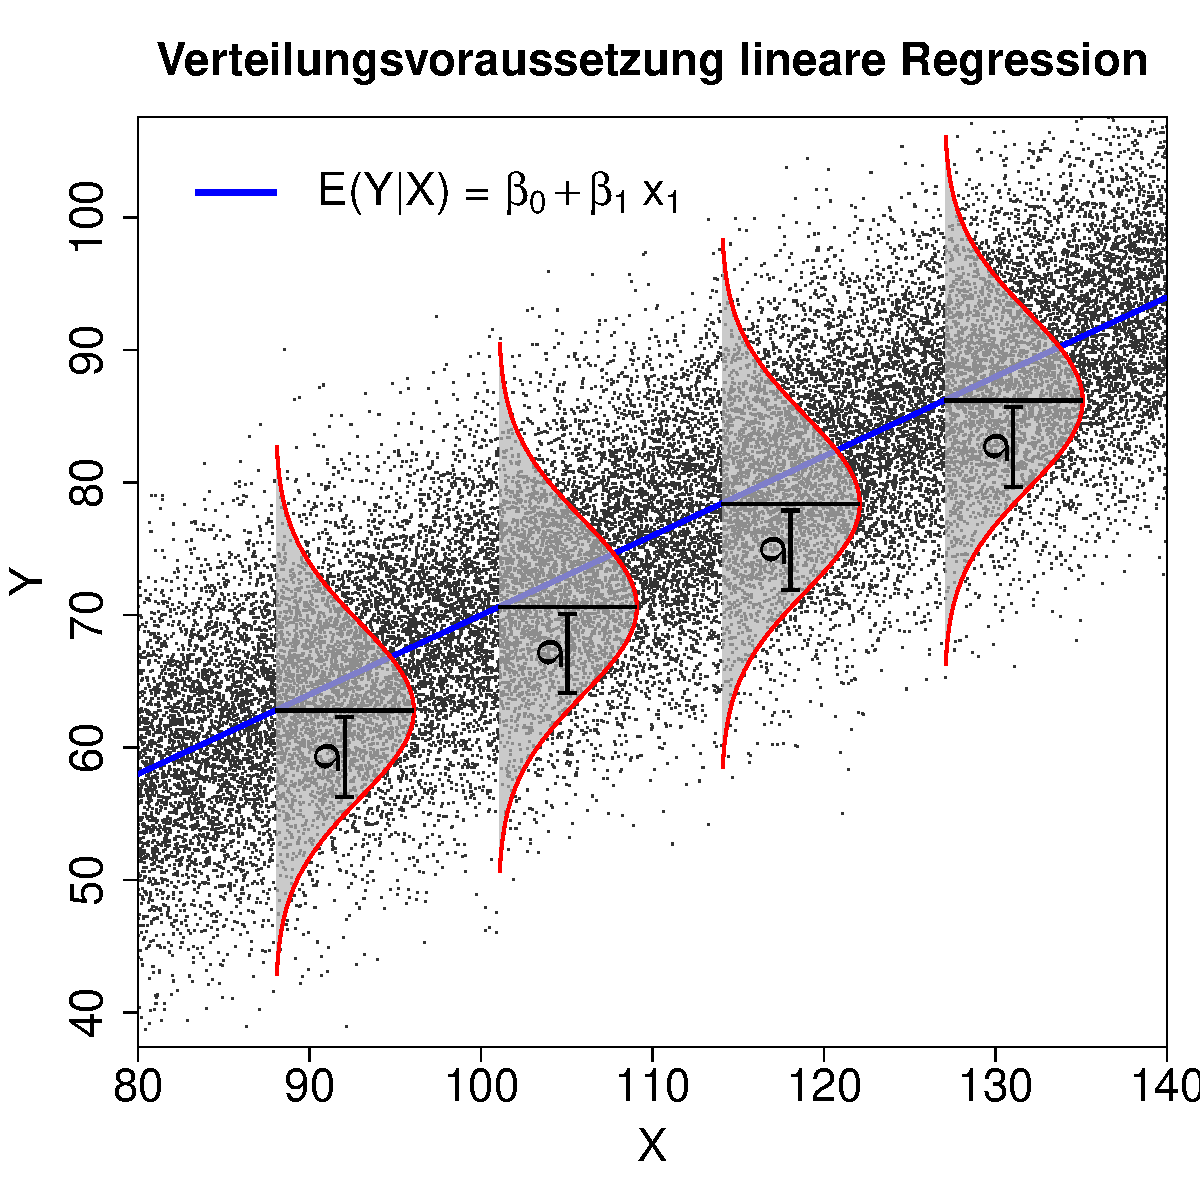
\includegraphics[width=8cm]{regrHomSc}
\vspace*{-1em}
\caption{Verteilungsvoraussetzungen im allgemeinen linearen Modell am Beispiel der einfachen linearen Regression}
\label{fig:regrHomSc}
\end{figure}

Der Vektor $\hat{\bm{\beta}}$ der i.\,S.\ der geringsten Quadratsumme der Residuen optimalen Parameterschätzungen ist gleich $\bm{X}^{+} \bm{y} = (\bm{X}^{\top} \bm{X})^{-1} \bm{X}^{\top} \bm{y}$.\footnote{\label{ftn:dummyCoef}In der Varianzanalyse werden die reduzierten Parameter geschätzt. Für die Beziehung zwischen geschätzten ursprünglichen Parametern und geschätzten reduzierten Parametern gilt $\hat{\bm{\beta}}^{\star} = [\bm{1} | \bm{C}] \, \hat{\bm{\beta}}$. Auf Basis eines mit \lstinline!aov()! oder \lstinline!lm()! angepassten linearen Modells erhält man $\hat{\bm{\beta}}$ mit\index[func]{coef()@\lstinline{coef()}} \lstinline!coef()! und $\hat{\bm{\beta}}^{\star}$ mit\index[func]{dummy.coef()@\lstinline{dummy.coef()}} \lstinline!dummy.coef()!.} Man erhält $\hat{\bm{\beta}}$ also als Koordinaten des Kriteriums, das orthogonal auf $V$ projiziert wurde, bzgl.\ der durch $\bm{X}$ definierten Basis (Abschn.\ \ref{sec:matOrthProj}). Es gilt $\hat{\bm{\beta}} \sim \bm{\mathcal{N}}(\bm{\beta}, \sigma^{2} (\bm{X}^{\top} \bm{X})^{-1})$, $\hat{\bm{\beta}}$ ist damit erwartungstreuer Schätzer für $\bm{\beta}$.\footnote{Zunächst ist $E(\hat{\bm{\beta}}) = E(\bm{X}^{+} \bm{y}) = \bm{X}^{+} E(\bm{y}) = (\bm{X}^{\top} \bm{X})^{-1} \bm{X}^{\top} \bm{X} \bm{\beta} = \bm{\beta}$. Weiter gilt $V(\hat{\bm{\beta}}) = V(\bm{X}^{+} \bm{y}) = \bm{X}^{+} V(\bm{y}) (\bm{X}^{+})^{\top} = (\bm{X}^{\top} \bm{X})^{-1} \bm{X}^{\top} \sigma^{2} \bm{I} \bm{X} (\bm{X}^{\top} \bm{X})^{-1} = \sigma^{2} (\bm{X}^{\top} \bm{X})^{-1}$.}

Der $n$-Vektor $\hat{\bm{y}} = (\hat{y}_{1}, \ldots, \hat{y}_{n})^{\top}$ der vorhergesagten Werte berechnet sich durch $\bm{X} \bm{X}^{+} \bm{y} = \bm{P} \bm{y}$, wobei die orthogonale Projektion $\bm{P} = \bm{X} (\bm{X}^{\top} \bm{X})^{-1} \bm{X}^{\top}$ auch als\index{allgemeines lineares Modell!Hat-Matrix} \emph{Hat-Matrix} bezeichnet wird. Man erhält $\hat{\bm{y}}$ also als Koordinaten des Kriteriums, das orthogonal auf $V$ projiziert wurde, bzgl.\ der Standardbasis. Die Vorhersage $\hat{\bm{y}}$ liegt damit in $V$.

Für den $n$-Vektor der Residuen $\bm{e} = (e_{1}, \ldots, e_{n})^{\top}$ gilt $\bm{e} = \bm{y} - \hat{\bm{y}} = \bm{I} \bm{y} - \bm{P} \bm{y} = (\bm{I} - \bm{P}) \bm{y}$. Die Residuen ergeben sich also als Projektion des Kriteriums auf das orthogonale Komplement von $V$. Die Residuen $\bm{e}$ liegen damit in $V^{\perp}$ und sind senkrecht zur Vorhersage. Der \emph{Fehlerraum} $V^{\perp}$ besitzt die Dimension $\text{Rang}(\bm{I}-\bm{P}) = n - \text{Rang}(\bm{X})$. Weiter gilt $E(\bm{e}) = \bm{0}$ und $V(\bm{e}) = \sigma^{2} (\bm{I} - \bm{P})$.\footnote{Zunächst ist $E(\bm{e}) = E((\bm{I} - \bm{P}) \bm{y}) = E(\bm{y}) - E(\bm{P} \bm{y}) = \bm{X} \bm{\beta} - \bm{P} \bm{X} \bm{\beta}$. Da die Spalten von $\bm{X}$ in $V$ liegen, bleiben sie durch $\bm{P}$ unverändert, es folgt also $E(\bm{e}) = \bm{X} \bm{\beta} - \bm{P} \bm{X} \bm{\beta} = \bm{0}$. Weiter gilt $V(\bm{e}) = V((\bm{I} - \bm{P}) \bm{y}) = (\bm{I} - \bm{P}) V(\bm{y}) (\bm{I} - \bm{P})^{\top} = \sigma^{2} (\bm{I} - \bm{P}) (\bm{I} - \bm{P})^{\top}$. Als orthogonale Projektion ist $\bm{I} - \bm{P}$ symmetrisch und idempotent, es gilt also $V(\bm{e}) = \sigma^{2} (\bm{I} - \bm{P}) (\bm{I} - \bm{P})^{\top} = \sigma^{2} (\bm{I} - \bm{P})$.}

Erwartungstreuer Schätzer für $\sigma^{2}$ ist die Quadratsumme der Residuen $SS_{e} = \|\bm{e}\|^{2} = \bm{y}^{\top} (\bm{I} - \bm{P}) \bm{y}$ geteilt durch die Anzahl der Fehler-Freiheitsgrade, die gleich der Dimension von $V^{\perp}$ ist.\footnote{\label{ftn:SSe}$SS_{e} = \sum_{i} e_{i}^{2} = \|\bm{e}\|^{2} = \bm{e}^{\top} \bm{e} = (\bm{y} - \hat{\bm{y}})^{\top} (\bm{y} - \hat{\bm{y}}) = \bm{y}^{\top} \bm{y} - \bm{y}^{\top} \hat{\bm{y}} - \hat{\bm{y}}^{\top} \bm{y} + \hat{\bm{y}}^{\top} \hat{\bm{y}} = \bm{y}^{\top} \bm{y} - \bm{y}^{\top} \bm{P} \bm{y} - (\bm{P} \bm{y})^{\top} \bm{y} + (\bm{P} \bm{y})^{\top} (\bm{P} \bm{y}) = \bm{y}^{\top} \bm{y} - \bm{y}^{\top} \bm{P} \bm{y} - \bm{y}^{\top} \bm{P} \bm{y} + \bm{y}^{\top} \bm{P} \bm{P} \bm{y} = \bm{y}^{\top} \bm{y} - \bm{y}^{\top} \bm{P} \bm{y} = \bm{y}^{\top} (\bm{I} - \bm{P}) \bm{y}$.} In der Regression mit $p$ Prädiktoren und absolutem Term ist $\hat{\sigma}^{2} = \frac{\|\bm{e}\|^{2}}{n-(p+1)}$ der quadrierte Standardschätzfehler, in der einfaktoriellen Varianzanalyse mit $p$ Gruppen ist $\hat{\sigma}^{2} = \frac{\|\bm{e}\|^{2}}{n-p}$ die mittlere Quadratsumme der Residuen.

Im multivariaten Fall werden mehrere Datenvektoren von Zielgrößen $\bm{y}_{l}$ spaltenweise zu einer Matrix $\bm{Y}$ zusammengestellt. Setzt man in den genannten Formeln $\bm{Y}$ für $\bm{y}$ ein, berechnen sich Parameterschätzungen, die spaltenweise aus den Vektoren der Vorhersagen $\hat{\bm{y}}_{l}$ zusammengestellte Matrix $\hat{\bm{Y}}$ und die spaltenweise aus den Vektoren der Residuen $\bm{e}_{l}$ zusammengestellte Matrix $\bm{E}$ wie in der univariaten Formulierung.

%%%%%%%%%%%%%%%%%%%%%%%%%%%%%%%%%%%%%%%%%%%%%%%%%%%%%%%%%%%%%%%%%%
%%%%%%%%%%%%%%%%%%%%%%%%%%%%%%%%%%%%%%%%%%%%%%%%%%%%%%%%%%%%%%%%%%
\subsection{Hypothesen über parametrische Funktionen testen}
\label{sec:multALMctr}
%%%%%%%%%%%%%%%%%%%%%%%%%%%%%%%%%%%%%%%%%%%%%%%%%%%%%%%%%%%%%%%%%%
%%%%%%%%%%%%%%%%%%%%%%%%%%%%%%%%%%%%%%%%%%%%%%%%%%%%%%%%%%%%%%%%%%

\index{allgemeines lineares Modell!parametrische Funktionen}
Im ALM können verschiedenartige Hypothesen über die Modellparameter $\beta_{j}$ getestet werden. Eine Gruppe solcher Hypothesen ist jene über den Wert einer \emph{parametrischen Funktion}. Im univariaten Fall ist eine parametrische Funktion $\psi = \sum_{j} c_{j} \beta_{j} = \bm{c}^{\top} \bm{\beta}$ eine Linearkombination der Parameter, wobei die Koeffizienten $c_{j}$ zu einem Vektor $\bm{c}$ zusammengestellt werden. Beispiele für parametrische Funktionen sind etwa a-priori Kontraste aus der Varianzanalyse (Abschn.\ \ref{sec:contrCRp}). Auch ein Parameter $\beta_{j}$ selbst (z.\,B.\ ein Gewicht in der Regression) ist eine parametrische Funktion, bei der $\bm{c}$ der $j$-te Einheitsvektor ist. Die $\text{H}_{0}$ lässt sich dann als $\psi = \psi_{0}$ mit einem festen Wert $\psi_{0}$ formulieren.

Eine parametrische Funktion wird mit Hilfe der Parameterschätzungen als $\hat{\psi} = \bm{c}^{\top} \hat{\bm{\beta}}$ erwartungstreu geschätzt, und es gilt $\hat{\psi} \sim \mathcal{N}(\psi, \sigma^{2} \bm{c}^{\top} (\bm{X}^{\top} \bm{X})^{-1} \bm{c})$.\footnote{Zunächst ist $E(\hat{\psi}) = E(\bm{c}^{\top} \hat{\bm{\beta}}) = \bm{c}^{\top} E(\hat{\bm{\beta}}) = \bm{c}^{\top} \bm{\beta} = \psi$. Weiter gilt $V(\hat{\psi}) = V(\bm{c}^{\top} \hat{\bm{\beta}}) = \bm{c}^{\top} V(\hat{\bm{\beta}}) \bm{c} = \bm{c}^{\top} \sigma^{2} (\bm{X}^{\top} \bm{X})^{-1} \bm{c}$. Bei $\hat{\psi}$ handelt es sich um einen \emph{Gauß-Markoff-Schätzer}, also den linearen erwartungstreuen Schätzer mit der geringsten Varianz.} $\hat{\psi}$ lässt sich auch direkt als Linearkombination der Beobachtungen $y_{i}$ im Vektor $\bm{y}$ formulieren:
\begin{equation*}
\hat{\psi} = \bm{c}^{\top} \hat{\bm{\beta}} = \bm{c}^{\top} (\bm{X}^{\top} \bm{X})^{-1} \bm{X}^{\top} \bm{y} = (\bm{X} (\bm{X}^{\top} \bm{X})^{-1} \bm{c})^{\top} \bm{y} = \bm{a}^{\top} \bm{y}
\end{equation*}

Dabei ist $\bm{a} = \bm{X} (\bm{X}^{\top} \bm{X})^{-1} \bm{c}$ der zu $\bm{c}$ gehörende $n$-Vektor der \emph{Schätzerkoeffizienten}, mit dem auch $\hat{\psi} = \bm{a}^{\top} \hat{\bm{y}}$\footnote{\label{ftn:estCoef}Zunächst ist $\bm{X}^{\top} \bm{a} = \bm{X}^{\top} \bm{X} (\bm{X}^{\top} \bm{X})^{-1} \bm{c} = \bm{c}$, also $\bm{c}^{\top} = \bm{a}^{\top} \bm{X}$. Damit gilt $\bm{a}^{\top} \bm{y} = \bm{c}^{\top} (\bm{X}^{\top} \bm{X})^{-1} \bm{X}^{\top} \bm{y} = \bm{a}^{\top} \bm{X} (\bm{X}^{\top} \bm{X})^{-1} \bm{X}^{\top} \bm{y} = \bm{a}^{\top} \bm{P} \bm{y} = \bm{a}^{\top} \hat{\bm{y}}$.} sowie $\sigma^{2}_{\hat{\psi}} = \bm{a}^{\top} \bm{a} \sigma^{2} = \|\bm{a}\|^{2} \sigma^{2}$ gilt.\footnote{$\|\bm{a}\|^{2} = \bm{a}^{\top} \bm{a} = (\bm{X} (\bm{X}^{\top} \bm{X})^{-1} \bm{c})^{\top} \bm{X} (\bm{X}^{\top} \bm{X})^{-1} \bm{c} = \bm{c}^{\top} (\bm{X}^{\top} \bm{X})^{-1} \bm{X}^{\top} \bm{X} (\bm{X}^{\top} \bm{X})^{-1} \bm{c} = \bm{c}^{\top} (\bm{X}^{\top} \bm{X})^{-1} \bm{c}$.} Damit lässt sich die $t$-Teststatistik in der üblichen Form $\frac{\hat{\psi} - \psi_{0}}{\hat{\sigma}_{\hat{\psi}}}$ definieren:
\begin{equation*}
t = \frac{\hat{\psi} - \psi_{0}}{\hat{\sigma} \sqrt{\bm{c}^{\top} (\bm{X}^{\top} \bm{X})^{-1} \bm{c}}} = \frac{\hat{\psi} - \psi_{0}}{\|\bm{a}\| \sqrt{\|\bm{e}\|^{2} / (n - \text{Rang}(\bm{X}))}}
\end{equation*}

Unter $\text{H}_{0}$ ist $t$ zentral $t$-verteilt mit $n - \text{Rang}(\bm{X})$ Freiheitsgraden (im Fall der Regression $n - (p+1)$, im Fall der einfaktoriellen Varianzanalyse ($n-p$)).

%%%%%%%%%%%%%%%%%%%%%%%%%%%%%%%%%%%%%%%%%%%%%%%%%%%%%%%%%%%%%%%%%%
%%%%%%%%%%%%%%%%%%%%%%%%%%%%%%%%%%%%%%%%%%%%%%%%%%%%%%%%%%%%%%%%%%
\subsection{Lineare Hypothesen als Modellvergleiche formulieren}
\label{sec:multALMmodCmp}
%%%%%%%%%%%%%%%%%%%%%%%%%%%%%%%%%%%%%%%%%%%%%%%%%%%%%%%%%%%%%%%%%%
%%%%%%%%%%%%%%%%%%%%%%%%%%%%%%%%%%%%%%%%%%%%%%%%%%%%%%%%%%%%%%%%%%

\index{allgemeines lineares Modell!Modellvergleiche}
\index{allgemeines lineares Modell!lineare Hypothesen}
Analog zur einzelnen parametrischen Funktion können Hypothesen über einen Vektor $\bm{\psi}$ von $m$ parametrischen Funktionen $\psi_{j} = \bm{c}_{j}^{\top} \bm{\beta}$ gleichzeitig formuliert werden, wobei die $\psi_{j}$ linear unabhängig sein sollen. Diese \emph{linearen} Hypothesen besitzen die Form $\bm{\psi} = \bm{L} \bm{\beta}$. Dabei ist $\bm{L}$ eine Matrix aus den zeilenweise zusammengestellten Koeffizientenvektoren $\bm{c}_{j}$ für die Linearkombinationen der allgemein $u$ Parameter im Vektor $\bm{\beta}$ ($u > m$). $\bm{L}$ ist dann eine $(m \times u)$-Matrix mit Rang $m$. Der unter $\text{H}_{0}$ für $\bm{\psi}$ angenommene Vektor sei $\bm{\psi}_{0}$.

Im multivariaten Fall mit $r$ Variablen $Y_{l}$ und der $(u \times r)$-Matrix der Parameter $\bm{B}$ hat eine lineare Hypothese die Form $\bm{\Psi} = \bm{L} \bm{B}$, wobei die unter $\text{H}_{0}$ für $\bm{\Psi}$ angenommene Matrix $\bm{\Psi}_{0}$ sei.

Die hier vorgestellten linearen Hypothesen aus der Varianzanalyse und Regression haben die Form $\bm{\psi}_{0} = \bm{0}$ (bzw.\ $\bm{\Psi}_{0} = \bm{0}$) und beziehen sich auf den Vergleich zweier nested Modelle (Abschn.\ \ref{sec:regrCmp}, \ref{sec:anova}): Das umfassendere (\emph{unrestricted}) $\text{H}_{1}$-Modell mit Designmatrix $\bm{X}_{u}$ besitzt dabei im univariaten Fall allgemein $u$ freie Parameter. Für das eingeschränkte (\emph{restricted}) $\text{H}_{0}$-Modell mit Designmatrix $\bm{X}_{r}$ nimmt man an, dass $m$ der Parameter des umfassenderen Modells $0$ sind, wodurch es noch $r = u-m$ freie Parameter besitzt. Man erhält $\bm{X}_{r}$, indem man die zu den auf $0$ gesetzten Parametern gehörenden $m$ Spalten von $\bm{X}_{u}$ streicht.

Die freien Parameter des eingeschränkten Modells bilden eine echte Teilmenge jener des umfassenderen Modells. Daher liegt der von den Spalten von $\bm{X}_{r}$ aufgespannte Unterraum $V_{r}$ der Vorhersage des eingeschränkten Modells vollständig in jenem des umfassenderen Modells $V_{u}$, dem Erzeugnis der Spalten von $\bm{X}_{u}$. Umgekehrt liegt der Fehlerraum des umfassenderen Modells $V_{u}^{\perp}$ vollständig in jenem des eingeschränkten Modells $V_{r}^{\perp}$. Die $\text{H}_{0}$ lässt sich auch so formulieren, dass $E(\bm{y})$ in $V_{r}$ liegt.

Im multivariaten Fall besitzt $\bm{B}$ allgemein $u$ Zeilen mit freien Parametern. Für das eingeschränkte $\text{H}_{0}$-Modell nimmt man an, dass $m$ Zeilen von $\bm{B}$ gleich $0$ sind. Dadurch besitzt $\bm{B}$ unter $\text{H}_{0}$ noch $r = u-m$ Zeilen mit freien Parametern. $\bm{X}_{u}$ und $\bm{X}_{r}$ stehen wie im univariaten Fall zueinander, unter $\text{H}_{0}$ soll also jede Spalte von $E(\bm{Y})$ in $V_{r}$ liegen. Für die inferenzstatistische Prüfung s.\ Abschn.\ \ref{sec:multALMtest}.

%%%%%%%%%%%%%%%%%%%%%%%%%%%%%%%%%%%%%%%%%%%%%%%%%%%%%%%%%%%%%%%%%%
%%%%%%%%%%%%%%%%%%%%%%%%%%%%%%%%%%%%%%%%%%%%%%%%%%%%%%%%%%%%%%%%%%
\subsubsection{Univariate einfaktorielle Varianzanalyse}
%%%%%%%%%%%%%%%%%%%%%%%%%%%%%%%%%%%%%%%%%%%%%%%%%%%%%%%%%%%%%%%%%%
%%%%%%%%%%%%%%%%%%%%%%%%%%%%%%%%%%%%%%%%%%%%%%%%%%%%%%%%%%%%%%%%%%

\index{Varianzanalyse!multivariate!einfaktorielle}
In der univariaten einfaktoriellen Varianzanalyse sind unter $\text{H}_{0}$ alle Gruppenerwartungswerte gleich. Dies ist äquivalent zur Hypothese, dass $\bm{\beta}_{p-1} = \bm{0}$, also $\bm{\beta} = (\beta_{0}, \bm{\beta}_{p-1}^{\top})^{\top} = (\beta_{0}, \bm{0}^{\top})^{\top}$ gilt. In $\text{H}_{0}: \bm{L} \bm{\beta} = \bm{0}$ hat $\bm{L}$ hier damit die Form $[\bm{0} | \bm{I}]$, wobei $\bm{0}$ der $(p-1)$-Vektor $(0, \ldots, 0)^{\top}$ und $\bm{I}$ die $((p-1) \times (p-1))$-Einheitsmatrix ist. Das $\text{H}_{0}$-Modell mit einem Parameter $\beta_{0}$ lässt sich als $E(\bm{y}) = \bm{1} \beta_{0}$ formulieren. Im umfassenderen $\text{H}_{1}$-Modell mit $p$ Parametern gibt es keine Einschränkung für $\bm{\beta}_{p-1}$, es ist damit identisch zum vollständigen Modell der einfaktoriellen Varianzanalyse $E(\bm{y}) = \bm{X} \bm{\beta}$: Hier ist also $u=p$, $\bm{X}_{u} = \bm{X}$, $r=1$, $\bm{X}_{r} = \bm{1}$ und $m = p-1$ (Abschn.\ \ref{sec:multALManova}).

%%%%%%%%%%%%%%%%%%%%%%%%%%%%%%%%%%%%%%%%%%%%%%%%%%%%%%%%%%%%%%%%%%
%%%%%%%%%%%%%%%%%%%%%%%%%%%%%%%%%%%%%%%%%%%%%%%%%%%%%%%%%%%%%%%%%%
\subsubsection{Univariate zweifaktorielle Varianzanalyse: Quadratsummen vom Typ I}
%%%%%%%%%%%%%%%%%%%%%%%%%%%%%%%%%%%%%%%%%%%%%%%%%%%%%%%%%%%%%%%%%%
%%%%%%%%%%%%%%%%%%%%%%%%%%%%%%%%%%%%%%%%%%%%%%%%%%%%%%%%%%%%%%%%%%

\index{Varianzanalyse!multivariate!zweifaktorielle}
\index{Varianzanalyse!Quadratsummen-Typen}
Wie in Abschn.\ \ref{sec:ssTypes} erläutert, existieren in der zweifaktoriellen Varianzanalyse (CRF-$pq$ Design) Typen von Quadratsummen, die bei ungleichen Zellbesetzungen zu unterschiedlichen Tests führen können. Proportional ungleiche Zellbesetzungen sind dabei gegeben, wenn $\frac{n_{jk}}{n_{jk'}} = \frac{n_{j'k}}{n_{j'k'}}$ sowie $\frac{n_{jk}}{n_{j'k}} = \frac{n_{jk'}}{n_{j'k'}}$ für alle $j, j', k, k'$ gilt. Ist dies nicht der Fall, spricht man von unbalancierten Zellbesetzungen.

Zunächst sind für den Test jedes Effekts (beide Haupteffekte und Interaktionseffekt) das eingeschränkte $\text{H}_{0}$-Modell sowie das umfassendere $\text{H}_{1}$-Modell zu definieren. Die $\text{H}_{0}$ des Haupteffekts des ersten Faktors lässt sich mit Hilfe des zugehörigen Parametervektors als $\bm{\beta}_{1} = \bm{0}$ formulieren. Bei Quadratsummen vom Typ I wählt man für den Test des Haupteffekts des ersten Faktors als $\text{H}_{0}$-Modell das Gesamt-Nullmodell, bei dem alle Parametervektoren $\bm{\beta}_{1}$, $\bm{\beta}_{2}$, $\bm{\beta}_{1 \times 2}$ gleich $\bm{0}$ sind und damit $E(\bm{y}) = \bm{1} \beta_{0}$ gilt. Hier gilt also für die Designmatrix des eingeschränkten Modells $\bm{X}_{r} = \bm{X}_{0} = \bm{1}$. Das sequentiell folgende $\text{H}_{1}$-Modell für den Test des ersten Faktors ist jenes, bei dem man die zugehörigen $p-1$ Parameter in $\bm{\beta}_{1}$ dem eingeschränkten Modell hinzufügt und die Designmatrix entsprechend erweitert, d.\,h.\ $\bm{X}_{u} = [\bm{1} | \bm{X}_{1}]$:
\begin{equation*}
E(\bm{y}) = [\bm{1} | \bm{X}_{1}] \left(\begin{array}{c} \beta_{0} \\ \bm{\beta}_{1} \end{array}\right)
\end{equation*}

Die $\text{H}_{0}$ des Haupteffekts des zweiten Faktors lautet mit Hilfe des zugehörigen Parametervektors $\bm{\beta}_{2} = \bm{0}$. Bei Quadratsummen vom Typ I fällt die Wahl für das $\text{H}_{0}$-Modell des zweiten Faktors auf das $\text{H}_{1}$-Modell des ersten Faktors ($\bm{X}_{r} = [\bm{1} | \bm{X}_{1}]$). Das $\text{H}_{1}$-Modell für den Test des zweiten Faktors ist jenes mit der sequentiell erweiterten Designmatrix $\bm{X}_{u} = [\bm{1} | \bm{X}_{1} | \bm{X}_{2}]$:
\begin{equation*}
E(\bm{y}) = [\bm{1} | \bm{X}_{1} | \bm{X}_{2}] \left(\begin{array}{c} \beta_{0} \\ \bm{\beta}_{1} \\ \bm{\beta}_{2}\end{array}\right)
\end{equation*}

Durch den sequentiellen Aufbau der Modellvergleiche ist die Reihenfolge der Gruppierungsfaktoren beim Test der Haupteffekte in Fällen mit unbalancierten Zellbesetzungen rechnerisch bedeutsam.

Die $\text{H}_{0}$ des Interaktionseffekts lautet mit Hilfe des zugehörigen Parametervektors $\bm{\beta}_{1 \times 2} = \bm{0}$. Die Wahl für das $\text{H}_{0}$-Modell der Interaktion ist das sequentielle $\text{H}_{1}$-Modell des zweiten Faktors ($\bm{X}_{r} = [\bm{1} | \bm{X}_{1} | \bm{X}_{2}]$). Das $\text{H}_{1}$-Modell der Interaktion ist das in Abschn.\ \ref{sec:multALManovaCRF} vorgestellte vollständige Modell der zweifaktoriellen Varianzanalyse ($\bm{X}_{u} = \bm{X}$):
\begin{equation*}
E(\bm{y}) = [\bm{1} | \bm{X}_{1} | \bm{X}_{2} | \bm{X}_{1 \times 2}] \left(\begin{array}{l} \beta_{0} \\ \bm{\beta}_{1}  \\ \bm{\beta}_{2} \\ \bm{\beta}_{1 \times 2}\end{array}\right) = \bm{X} \bm{\beta}
\end{equation*}

In $\text{H}_{0}: \bm{L} \bm{\beta} = \bm{0}$ hat $\bm{L}$ in den genannten Tests der Haupteffekte die Form $[\bm{0} | \bm{I} | \bm{0}]$ und beim Test der Interaktion die Form $[\bm{0} | \bm{I}]$. Dabei ist $\bm{I}$ der Reihe nach die $((p-1) \times (p-1))$-, $((q-1) \times (q-1))$- und $((p-1) \cdot (q-1) \times (p-1) \cdot (q-1))$-Einheitsmatrix und $\bm{0}$ eine passende Matrix aus $0$-Einträgen.

%%%%%%%%%%%%%%%%%%%%%%%%%%%%%%%%%%%%%%%%%%%%%%%%%%%%%%%%%%%%%%%%%%
%%%%%%%%%%%%%%%%%%%%%%%%%%%%%%%%%%%%%%%%%%%%%%%%%%%%%%%%%%%%%%%%%%
\subsubsection{Zweifaktorielle Varianzanalyse: Quadratsummen vom Typ II}
%%%%%%%%%%%%%%%%%%%%%%%%%%%%%%%%%%%%%%%%%%%%%%%%%%%%%%%%%%%%%%%%%%
%%%%%%%%%%%%%%%%%%%%%%%%%%%%%%%%%%%%%%%%%%%%%%%%%%%%%%%%%%%%%%%%%%

Auch bei Quadratsummen vom Typ II unterscheiden sich die eingeschränkten und umfassenderen Modelle um jeweils $p-1$ (erster Haupteffekt), $q-1$ (zweiter Haupteffekt) und $(p-1) \cdot (q-1)$ (Interaktion) freie Parameter. Das $\text{H}_{1}$-Modell beim Test beider Haupteffekte ist hier:
\begin{equation*}
E(\bm{y}) = [\bm{1} | \bm{X}_{1} | \bm{X}_{2}] \left(\begin{array}{l} \beta_{0} \\ \bm{\beta}_{1} \\ \bm{\beta}_{2}\end{array}\right)
\end{equation*}

Das jeweilige $\text{H}_{0}$-Modell für den Test des Haupteffekts eines Faktors wird bei Quadratsummen vom Typ II dadurch gebildet, dass ausgehend vom $\text{H}_{1}$-Modell die Parameter des zu testenden Effekts auf $0$ gesetzt und die zugehörigen Spalten der Designmatrix entfernt werden.
\begin{align*}
E(\bm{y}) &= [\bm{1} | \bm{X}_{2}] \left(\begin{array}{l} \beta_{0} \\ \bm{\beta}_{2}\end{array}\right) && (\text{H}_{0}-\text{Modell für Test Faktor 1}) \\
E(\bm{y}) &= [\bm{1} | \bm{X}_{1}] \left(\begin{array}{l} \beta_{0} \\ \bm{\beta}_{1}\end{array}\right) && (\text{H}_{0}-\text{Modell für Test Faktor 2})
\end{align*}

Die Reihenfolge der Faktoren ist anders als bei Quadratsummen vom Typ I beim Test der Haupteffekte unwesentlich, selbst wenn unbalancierte Zellbesetzungen vorliegen. Liegen proportional ungleiche Zellbesetzungen vor, stimmen die Ergebnisse für den Test der Haupteffekte mit jenen aus Quadratsummen vom Typ I überein. Bei Quadratsummen vom Typ II ist die Wahl für $\text{H}_{0}$- und $\text{H}_{1}$-Modell beim Test der Interaktion gleich jener bei Quadratsummen vom Typ I und III, die Ergebnisse sind daher identisch.

%%%%%%%%%%%%%%%%%%%%%%%%%%%%%%%%%%%%%%%%%%%%%%%%%%%%%%%%%%%%%%%%%%
%%%%%%%%%%%%%%%%%%%%%%%%%%%%%%%%%%%%%%%%%%%%%%%%%%%%%%%%%%%%%%%%%%
\subsubsection{Zweifaktorielle Varianzanalyse: Quadratsummen vom Typ III}
%%%%%%%%%%%%%%%%%%%%%%%%%%%%%%%%%%%%%%%%%%%%%%%%%%%%%%%%%%%%%%%%%%
%%%%%%%%%%%%%%%%%%%%%%%%%%%%%%%%%%%%%%%%%%%%%%%%%%%%%%%%%%%%%%%%%%

Auch bei Quadratsummen vom Typ III unterscheiden sich die eingeschränkten und umfassenderen Modelle um jeweils $p-1$ (erster Haupteffekt), $q-1$ (zweiter Haupteffekt) und $(p-1) \cdot (q-1)$ (Interaktion) freie Parameter. Hier ist beim Test aller Effekte das $\text{H}_{1}$-Modell das in Abschn.\ \ref{sec:multALManovaCRF} vorgestellte vollständige Modell der zweifaktoriellen Varianzanalyse:
\begin{equation*}
E(\bm{y}) = [\bm{1} | \bm{X}_{1} | \bm{X}_{2} | \bm{X}_{1 \times 2}] \left(\begin{array}{l} \beta_{0} \\ \bm{\beta}_{1} \\ \bm{\beta}_{2} \\ \bm{\beta}_{1 \times 2}\end{array}\right) = \bm{X} \bm{\beta}
\end{equation*}

Das jeweilige $\text{H}_{0}$-Modell für den Test aller Effekte wird bei Quadratsummen vom Typ III dadurch gebildet, dass ausgehend vom vollständigen Modell die Parameter des zu testenden Effekts auf $0$ gesetzt und die zugehörigen Spalten der Designmatrix gestrichen werden:
\begin{align*}
E(\bm{y}) &= [\bm{1} | \bm{X}_{2} | \bm{X}_{1 \times 2}] \left(\begin{array}{l} \beta_{0} \\ \bm{\beta}_{2} \\ \bm{\beta}_{1 \times 2}\end{array}\right) && (\text{H}_{0}-\text{Modell für Test Faktor 1}) \\
E(\bm{y}) &= [\bm{1} | \bm{X}_{1} | \bm{X}_{1 \times 2}] \left(\begin{array}{l} \beta_{0} \\ \bm{\beta}_{1} \\ \bm{\beta}_{1 \times 2}\end{array}\right) && (\text{H}_{0}-\text{Modell für Test Faktor 2}) \\
E(\bm{y}) &= [\bm{1} | \bm{X}_{1} | \bm{X}_{2}] \left(\begin{array}{l} \beta_{0} \\ \bm{\beta}_{1} \\ \bm{\beta}_{2}\end{array}\right) && (\text{H}_{0}-\text{Modell für Test Interaktion})
\end{align*}

Die Reihenfolge der Faktoren ist anders als bei Quadratsummen vom Typ I beim Test der Haupteffekte unwesentlich, selbst wenn unbalancierte Zellbesetzungen vorliegen. Bei gleichen Zellbesetzungen liefern alle drei Typen von Quadratsummen dieselben Ergebnisse. Bei Quadratsummen vom Typ III stimmt die Wahl für $\text{H}_{0}$- und $\text{H}_{1}$-Modell beim Test der Interaktion mit jener bei Quadratsummen vom Typ I und II überein, die Ergebnisse sind daher identisch. Ein Test des absoluten Terms $\beta_{0}$ ist mit Quadratsummen vom Typ III ebenso wenig möglich wie ein Test von Haupteffekten, die nicht Teil einer Interaktion sind.

Die $\text{H}_{0}$-Modelle für Haupteffekte machen bei Quadratsummen vom Typ III keine Einschränkung für den Parametervektor $\bm{\beta}_{1 \times 2}$ der Interaktion, obwohl die Parameter des zu testenden, und an der Interaktion beteiligten Haupteffekts auf $0$ gesetzt werden. Die Modellvergleiche verletzen damit anders als bei Quadratsummen vom Typ I und II das Prinzip, dass Vorhersageterme höherer Ordnung nur in das Modell aufgenommen werden, wenn alle zugehörigen Terme niederer Ordnung ebenfalls Berücksichtigung finden.

Modellvergleiche für Quadratsummen vom Typ III können deshalb bei ungleichen Zellbesetzungen in Abhängigkeit von der verwendeten Nebenbedingung für die Parameter samt Codierschema unterschiedlich ausfallen \cite{Venables2016}. Richtige Ergebnisse erhält man mit $\bm{v} = \bm{1}$, was alle Codierschemata gewährleisten, deren Koeffizienten sich über die Spalten der Codiermatrix $\bm{C}$ zu $0$ summieren (Abschn.\ \ref{sec:multALManova}). Dazu zählen Effekt- und Helmert-Codierung, nicht aber Treatment-Kontraste (Dummy-Codierung) -- die Voreinstellung in R. Bei Quadratsummen vom Typ I und II spielt die Wahl von Nebenbedingung und Codierschema dagegen keine Rolle für den inferenzstatistischen Test.

%%%%%%%%%%%%%%%%%%%%%%%%%%%%%%%%%%%%%%%%%%%%%%%%%%%%%%%%%%%%%%%%%%
%%%%%%%%%%%%%%%%%%%%%%%%%%%%%%%%%%%%%%%%%%%%%%%%%%%%%%%%%%%%%%%%%%
\subsubsection{Multiple Regression}
%%%%%%%%%%%%%%%%%%%%%%%%%%%%%%%%%%%%%%%%%%%%%%%%%%%%%%%%%%%%%%%%%%
%%%%%%%%%%%%%%%%%%%%%%%%%%%%%%%%%%%%%%%%%%%%%%%%%%%%%%%%%%%%%%%%%%

Die Modellvergleiche beim Test von $p$ Prädiktoren $X_{j}$ in der multiplen Regression werden nach demselben Prinzip wie in der zweifaktoriellen Varianzanalyse gebildet: Das Gesamt-Nullmodell ist $E(\bm{Y}) = \bm{1} \bm{\beta}_{0}^{\top}$, bei dem für alle Kriterien $\bm{y}_{l}$ der zugehörige Parametervektor der $p$ Prädiktoren $\bm{\beta}_{p.l} = \bm{0}$ und damit $\bm{B}_{p.0} = \bm{0}$ sowie $\bm{X}_{0} = \bm{1}$ ist. Das vollständige Modell ist jenes mit allen Prädiktoren $E(\bm{Y}) = \bm{X} \bm{B}$.

Die Prädiktoren werden über Modellvergleiche getestet, die wie in der zweifaktoriellen Varianzanalyse vom verwendeten Typ der Quadratsummen abhängen. Die Reihenfolge der Prädiktoren ist im multivariaten Fall bei Quadratsummen vom Typ I bedeutsam, sofern nicht alle Prädiktoren paarweise unkorreliert sind: Für den Test des ersten Prädiktors ist das eingeschränkte $\text{H}_{0}$-Modell das Gesamt-Nullmodell, das zugehörige umfassendere $\text{H}_{1}$-Modell ist jenes mit nur dem ersten Prädiktor. Für den Test des zweiten Prädiktors ist das eingeschränkte $\text{H}_{0}$-Modell das sequentielle $\text{H}_{1}$-Modell des ersten Prädiktors, das $\text{H}_{1}$-Modell ist jenes mit den ersten beiden Prädiktoren. Für die Tests aller folgenden Prädiktoren gilt dies analog.

Bei Quadratsummen vom Typ II ist das $\text{H}_{1}$-Modell beim Test aller Prädiktoren gleich dem vollständigen Modell mit allen Prädiktoren, jedoch ohne deren Interaktionen. Das $\text{H}_{0}$-Modell beim Test eines Prädiktors $X_{j}$ entsteht aus dem $\text{H}_{1}$-Modell, indem der zu $X_{j}$ gehörende Parametervektor $\bm{\beta}_{j}^{\top} = \bm{0}^{\top}$ gesetzt und die passende Spalte der Designmatrix gestrichen wird.

Bei Quadratsummen vom Typ III ist das $\text{H}_{1}$-Modell beim Test aller Prädiktoren gleich dem vollständigen Modell mit allen Prädiktoren und deren Interaktionen, sofern letztere berücksichtigt werden sollen. Das $\text{H}_{0}$-Modell beim Test eines Prädiktors $X_{j}$ entsteht aus dem $\text{H}_{1}$-Modell, indem der zu $X_{j}$ gehörende Parametervektor $\bm{\beta}_{j}^{\top} = \bm{0}^{\top}$ gesetzt und die passende Spalte der Designmatrix gestrichen wird. Quadratsummen vom Typ II und III unterscheiden sich also nur, wenn die Regression auch Interaktionsterme einbezieht.

Sollen allgemein die Parameter von $m$ Prädiktoren gleichzeitig daraufhin getestet werden, ob sie $0$ sind, ist das Vorgehen analog, wobei unter $\text{H}_{0}$ die zugehörigen, aus $\bm{B}$ stammenden $m$ Parametervektoren $\bm{\beta}_{j}^{\top} = \bm{0}^{\top}$ gesetzt und entsprechend ausgehend vom $\text{H}_{1}$-Modell die passenden Spalten der Designmatrix gestrichen werden.

%%%%%%%%%%%%%%%%%%%%%%%%%%%%%%%%%%%%%%%%%%%%%%%%%%%%%%%%%%%%%%%%%%
%%%%%%%%%%%%%%%%%%%%%%%%%%%%%%%%%%%%%%%%%%%%%%%%%%%%%%%%%%%%%%%%%%
% TODO
%\subsubsection{Kovarianzanalyse}
%%%%%%%%%%%%%%%%%%%%%%%%%%%%%%%%%%%%%%%%%%%%%%%%%%%%%%%%%%%%%%%%%%
%%%%%%%%%%%%%%%%%%%%%%%%%%%%%%%%%%%%%%%%%%%%%%%%%%%%%%%%%%%%%%%%%%

%%%%%%%%%%%%%%%%%%%%%%%%%%%%%%%%%%%%%%%%%%%%%%%%%%%%%%%%%%%%%%%%%%
%%%%%%%%%%%%%%%%%%%%%%%%%%%%%%%%%%%%%%%%%%%%%%%%%%%%%%%%%%%%%%%%%%
\subsection{Lineare Hypothesen testen}
\label{sec:multALMtest}
%%%%%%%%%%%%%%%%%%%%%%%%%%%%%%%%%%%%%%%%%%%%%%%%%%%%%%%%%%%%%%%%%%
%%%%%%%%%%%%%%%%%%%%%%%%%%%%%%%%%%%%%%%%%%%%%%%%%%%%%%%%%%%%%%%%%%

Liegt eine lineare Hypothese der Form $\bm{\psi} = \bm{L} \bm{\beta}$ vor \cite{Fox2013}, soll $\bm{A}$ die zur $((u-r) \times u)$-Matrix $\bm{L}$ gehörende $((u-r) \times n)$-Matrix bezeichnen, die zeilenweise aus den $n$-Vektoren der Schätzerkoeffizienten $\bm{a}_{j} = \bm{X}_{u} (\bm{X}_{u}^{\top} \bm{X}_{u})^{-1} \bm{c}_{j}$ gebildet wird (Abschn.\ \ref{sec:multALMctr}). Es gilt also $\bm{A}^{\top} = \bm{X}_{u} (\bm{X}_{u}^{\top} \bm{X}_{u})^{-1} \bm{L}^{\top}$ und $\text{Rang}(\bm{A}) = \text{Rang}(\bm{L}) = u-r$. Aus $\bm{c} = \bm{X}^{\top} \bm{a}$ (Abschn.\ \ref{sec:multALMmodCmp}, Fußnote \ref{ftn:estCoef}) folgt damit $\bm{L}^{\top} = \bm{X}_{u}^{\top} \bm{A}^{\top}$, also $\bm{L} = \bm{A} \bm{X}_{u}$.\footnote{$\bm{A} \bm{X}_{u} = (\bm{X}_{u} (\bm{X}_{u}^{\top} \bm{X}_{u})^{-1} \bm{L}^{\top})^{\top} \bm{X}_{u} = \bm{L} (\bm{X}_{u}^{\top} \bm{X}_{u})^{-1} \bm{X}_{u}^{\top} \bm{X}_{u} = \bm{L}$.}

Der Vektor der Schätzungen $\hat{\bm{\psi}} = \bm{L} \hat{\bm{\beta}}$ kann mit $\bm{A}$ analog zur Schätzung einer einfachen parametrischen Funktion $\hat{\psi}_{j} = \bm{c}_{j}^{\top} \hat{\bm{\beta}} = \bm{a}_{j}^{\top} \bm{y}$ auch als Abbildung des Vektors der Beobachtungen $\bm{y}$ formuliert werden:
\begin{equation*}
\hat{\bm{\psi}} = \bm{L} \hat{\bm{\beta}} = \bm{L} (\bm{X}_{u}^{\top} \bm{X}_{u})^{-1} \bm{X}_{u}^{\top} \bm{y} = \bm{A} \bm{y}
\end{equation*}

Mit der Vorhersage $\hat{\bm{y}}$ gilt zudem $\hat{\bm{\psi}} = \bm{A} \hat{\bm{y}}$.\footnote{\label{ftn:estCoeffMat}$\hat{\bm{\psi}} = \bm{L} \hat{\bm{\beta}} = \bm{L} (\bm{X}_{u}^{\top} \bm{X}_{u})^{-1} \bm{X}_{u}^{\top} \bm{y} = \bm{A} \bm{X}_{u} (\bm{X}_{u}^{\top} \bm{X}_{u})^{-1} \bm{X}_{u}^{\top} \bm{y} = \bm{A} \hat{\bm{y}}$.} $\hat{\bm{\psi}}$ ist ein erwartungstreuer Gauß-Markoff-Schätzer mit Verteilung $\hat{\bm{\psi}} \sim \bm{\mathcal{N}}(\bm{\psi}, \sigma^{2} \bm{A} \bm{A}^{\top})$.\footnote{\label{ftn:varPsiHat}Zunächst gilt $E(\bm{L} \hat{\bm{\beta}}) = \bm{L} E(\hat{\bm{\beta}}) = \bm{L} \bm{\beta} = \bm{\psi}$. Weiter ist $V(\hat{\bm{\psi}}) = V(\bm{L} \hat{\bm{\beta}}) = \bm{L} V(\hat{\bm{\beta}}) \bm{L}^{\top} = \sigma^{2} \bm{L} (\bm{X}_{u}^{\top} \bm{X}_{u})^{-1} \bm{L}^{\top} = \sigma^{2} \bm{L} (\bm{X}_{u}^{\top} \bm{X}_{u})^{-1} \bm{X}_{u}^{\top} \bm{X}_{u} (\bm{X}_{u}^{\top} \bm{X}_{u})^{-1} \bm{L}^{\top} = \sigma^{2} \bm{A} \bm{A}^{\top}$. Insbesondere ist also $\bm{A} \bm{A}^{\top} = \bm{L} (\bm{X}_{u}^{\top} \bm{X}_{u})^{-1} \bm{L}^{\top}$.} Der Rang der Kovarianzmatrix $\bm{\Sigma}_{\hat{\bm{\psi}}} = \sigma^{2} \bm{A} \bm{A}^{\top}$ beträgt $u-r$. Er ist also gleich der Differenz der Anzahl zu schätzender Parameter beider Modelle sowie gleich der Differenz der Dimensionen von $V_{u}$ und $V_{r}$ einerseits und von $V_{r}^{\perp}$ und $V_{u}^{\perp}$ andererseits.

%%%%%%%%%%%%%%%%%%%%%%%%%%%%%%%%%%%%%%%%%%%%%%%%%%%%%%%%%%%%%%%%%%
%%%%%%%%%%%%%%%%%%%%%%%%%%%%%%%%%%%%%%%%%%%%%%%%%%%%%%%%%%%%%%%%%%
\subsubsection{Univariate Teststatistik}
%%%%%%%%%%%%%%%%%%%%%%%%%%%%%%%%%%%%%%%%%%%%%%%%%%%%%%%%%%%%%%%%%%
%%%%%%%%%%%%%%%%%%%%%%%%%%%%%%%%%%%%%%%%%%%%%%%%%%%%%%%%%%%%%%%%%%

\index{allgemeines lineares Modell!Modellvergleiche}
Um die Teststatistik für den univariaten Fall zu motivieren, ist zunächst festzustellen, dass für die quadrierte Mahalanobisdistanz (Abschn.\ \ref{sec:mahaDist}) $\|\hat{\bm{\psi}} - \bm{\psi}_{0}\|_{M, \bm{\Sigma}_{\hat{\bm{\psi}}}}^{2}$ von $\hat{\bm{\psi}}$ zu $\bm{\psi}_{0} = \bm{0}$ bzgl.\ $\bm{\Sigma}_{\hat{\bm{\psi}}}$ gilt (Fußnoten \ref{ftn:estCoeffMat} und \ref{ftn:varPsiHat}):
\begin{alignat*}{2}
\|\hat{\bm{\psi}} - \bm{\psi}_{0}\|_{M, \bm{\Sigma}_{\hat{\bm{\psi}}}}^{2} &= (\hat{\bm{\psi}} - \bm{0})^{\top} \bm{\Sigma}_{\hat{\bm{\psi}}}^{-1} (\hat{\bm{\psi}} - \bm{0}) & &= \frac{\hat{\bm{\psi}}^{\top} (\bm{L} (\bm{X}_{u}^{\top} \bm{X}_{u})^{-1} \bm{L}^{\top})^{-1} \hat{\bm{\psi}}}{\sigma^{2}}\\[2ex]
 &= \frac{\hat{\bm{\psi}}^{\top} (\bm{A} \bm{A}^{\top})^{-1} \hat{\bm{\psi}}}{\sigma^{2}} & &= \frac{\bm{y}^{\top} \bm{A}^{\top} (\bm{A} \bm{A}^{\top})^{-1} \bm{A} \bm{y}}{\sigma^{2}}
\end{alignat*}

Hier ist $\bm{A}^{\top} (\bm{A} \bm{A}^{\top})^{-1} \bm{A}$ die Projektion auf das orthogonale Komplement von $V_{r}$ in $V_{u}$ (also $V_{r}^{\perp} \cap V_{u}$), dessen spaltenweise Basis $\bm{A}^{\top}$ ist.\footnote{Es sei $\bm{y}_{r} = \bm{X}_{u} \bm{r}$ aus $V_{r}$ und $\bm{y}_{a} = \bm{A}^{\top} \bm{a}$ aus dem Erzeugnis der Spalten von $\bm{A}^{\top}$ mit $\bm{r}$ und $\bm{a}$ als zugehörigen Koordinatenvektoren bzgl.\ $\bm{X}_{u}$ und $\bm{A}^{\top}$. Mit $\bm{A}^{\top} = \bm{X}_{u} (\bm{X}_{u}^{\top} \bm{X}_{u})^{-1} \bm{L}^{\top}$ liegt $\bm{y}_{a}$ als Linearkombination der Spalten von $\bm{X}_{u}$ in $V_{u}$. Da $\bm{y}_{r}$ in $V_{r}$ liegt, gilt $\bm{L} \bm{y}_{r} = \bm{0}$. Damit folgt $\bm{y}_{a}^{\top} \bm{y}_{r} = (\bm{A}^{\top} \bm{a})^{\top} \bm{X}_{u} \bm{r} = \bm{a}^{\top} \bm{A} \bm{X}_{u} \bm{r} = \bm{a}^{\top} \bm{L} (\bm{X}_{u}^{\top} \bm{X}_{u})^{-1} \bm{X}_{u}^{\top} \bm{X}_{u} \bm{r} = \bm{a}^{\top} \bm{L} \bm{r} = \bm{a}^{\top} \bm{0} = 0$, d.\,h.\ $\bm{y}_{a} \perp \bm{y}_{r}$. Also liegt $\bm{y}_{a}$ auch in $V_{r}^{\perp}$.}

Für die Schätzung der Fehlervarianz $\sigma^{2}$ benötigt man das vollständige (\emph{full}) Modell mit Designmatrix $\bm{X}_{f}$ und Projektionsmatrix $\bm{P}_{f}$ (bisher einfach als $\bm{X}$ und $\bm{P}$ bezeichnet), das alle Parameter beinhaltet. Der zugehörige Vektor der Residuen sei $\bm{e}_{f} = \bm{y} - \hat{\bm{y}}_{f}$, die Residual-Quadratsumme also $SS_{ef} = \|\bm{e}_{f}\|^{2}$ mit Freiheitsgraden $df_{ef} = n - \text{Rang}(\bm{X}_{f})$, der Dimension des Fehlerraumes $V_{f}^{\perp}$ (Abschn.\ \ref{sec:multALMpred}). Als erwartungstreuer Schätzer $\hat{\sigma}^{2}$ dient in allen Tests $SS_{ef} / df_{ef} = \bm{y}^{\top} (\bm{I} - \bm{P}_{f}) \bm{y} / (n - \text{Rang}(\bm{X}_{f}))$ (Abschn.\ \ref{sec:multALMctr}, Fußnote \ref{ftn:SSe}) -- also auch dann, wenn das umfassendere Modell nicht mit dem vollständigen Modell übereinstimmt. Damit lassen sich lineare Nullhypothesen $\bm{L} \bm{\beta} = \bm{0}$ im univariaten Fall mit der folgenden Teststatistik prüfen:
\begin{align*}
F &= \frac{\hat{\bm{\psi}}^{\top} (\bm{L} (\bm{X}_{u}^{\top} \bm{X}_{u})^{-1} \bm{L}^{\top})^{-1} \hat{\bm{\psi}} / \text{Rang}(\bm{\Sigma}_{\hat{\bm{\psi}}})}{\hat{\sigma}^{2}} = \frac{\hat{\bm{\psi}}^{\top} (\bm{A} \bm{A}^{\top})^{-1} \hat{\bm{\psi}} / (u - r)}{\hat{\sigma}^{2}}\\[2ex]
 &= \frac{\bm{y}^{\top} \bm{A}^{\top} (\bm{A} \bm{A}^{\top})^{-1} \bm{A} \bm{y} / (\text{Rang}(\bm{X}_{u}) - \text{Rang}(\bm{X}_{r}))}{\bm{y}^{\top} (\bm{I} - \bm{P}_{f}) \bm{y} / (n - \text{Rang}(\bm{X}_{f}))}
\end{align*}

Unter $\text{H}_{0}$ ist $F$ zentral $F$-verteilt mit $\text{Rang}(\bm{X}_{u}) - \text{Rang}(\bm{X}_{r})$ Zähler- und $n - \text{Rang}(\bm{X}_{f})$ Nenner-Freiheitsgraden. Das Modell einer Regression mit $p$ Prädiktoren und absolutem Term hat $n - (p+1)$ Fehler-Freiheitsgrade, das Modell einer einfaktoriellen Varianzanalyse mit $p$ Gruppen $n-p$.

Der Zähler der Teststatistik lässt sich äquivalent umformulieren, wobei explizit Bezug zum Modellvergleich genommen wird. Dafür sei $\bm{e}_{r}$ der Vektor der Residuen des eingeschränkten Modells mit zugehöriger Projektionsmatrix $\bm{P}_{r}$ und analog $\bm{e}_{u}$ der Vektor der Residuen des umfassenderen Modells mit Projektionsmatrix $\bm{P}_{u}$. In der einfaktoriellen Varianzanalyse sowie im Gesamt-Test der Regressionsanalyse sind das umfassendere Modell und das vollständige Modell identisch ($\bm{P}_{u} = \bm{P}_{f}$), ebenso ist dort das eingeschränkte Modell gleich dem Gesamt-Nullmodell ($\bm{P}_{r} = \bm{P}_{0}$).

Dann ist die Residual-Quadratsumme des eingeschränkten Modells $SS_{er} = \bm{y}^{\top} (\bm{I} - \bm{P}_{r}) \bm{y}$ mit Freiheitsgraden $df_{er} = n - \text{Rang}(\bm{X}_{r})$ und die des umfassenderen Modells $SS_{eu} = \bm{y}^{\top} (\bm{I} - \bm{P}_{u}) \bm{y}$ mit Freiheitsgraden $df_{eu} = n - \text{Rang}(\bm{X}_{u})$. Für die Differenz dieser Quadratsummen gilt $SS_{er} - SS_{eu} = \bm{y}^{\top} (\bm{P}_{u} - \bm{P}_{r}) \bm{y}$, wobei ihre Dimension $df_{er} - df_{eu} = \text{Rang}(\bm{X}_{u}) - \text{Rang}(\bm{X}_{r})$ und $\bm{P}_{u} - \bm{P}_{r} = \bm{A}^{\top} (\bm{A} \bm{A}^{\top})^{-1} \bm{A}$ ist. Damit lautet die Teststatistik:
\begin{align*}
F &= \frac{\bm{y}^{\top} (\bm{P}_{u} - \bm{P}_{r}) \bm{y} / (\text{Rang}(\bm{X}_{u}) - \text{Rang}(\bm{X}_{r}))}{\bm{y}^{\top} (\bm{I} - \bm{P}_{f}) \bm{y} / (n - \text{Rang}(\bm{X}_{f}))}\\[2ex]
  &= \frac{(SS_{er} - SS_{eu}) / (df_{er} - df_{eu})}{SS_{ef} / df_{ef}}
\end{align*}

%%%%%%%%%%%%%%%%%%%%%%%%%%%%%%%%%%%%%%%%%%%%%%%%%%%%%%%%%%%%%%%%%%
%%%%%%%%%%%%%%%%%%%%%%%%%%%%%%%%%%%%%%%%%%%%%%%%%%%%%%%%%%%%%%%%%%
\subsubsection{Multivariate Teststatistiken}
%%%%%%%%%%%%%%%%%%%%%%%%%%%%%%%%%%%%%%%%%%%%%%%%%%%%%%%%%%%%%%%%%%
%%%%%%%%%%%%%%%%%%%%%%%%%%%%%%%%%%%%%%%%%%%%%%%%%%%%%%%%%%%%%%%%%%

Die Quadratsummen des univariaten Falls verallgemeinern sich im multivariaten Fall zu folgenden Matrizen, auf denen letztlich die Teststatistiken basieren \cite{Fox2013}:

\begin{itemize}
\item $\bm{T} = \bm{Y}^{\top} (\bm{I} - \bm{P}_{0}) \bm{Y}$: Dies ist gleich der SSP-Matrix der Residuen des Gesamt-Nullmodells und damit gleich der SSP-Matrix der Gesamt-Daten.\footnote{\label{ftn:ssp}$\bm{X}_{0} = \bm{1}$, daher ist die Matrix der Residuen $\bm{E} = (\bm{I} - \bm{P}_{0}) \bm{Y} = \bm{Q} \bm{Y}$ zentriert (Abschn.\ \ref{sec:matOrthProj}, Fußnote \ref{ftn:ones}) und $(\bm{Q} \bm{Y})^{\top} (\bm{Q} \bm{Y})$ deren SSP-Matrix. Als orthogonale Projektion ist $\bm{Q}$ symmetrisch und idempotent, weshalb $(\bm{Q} \bm{Y})^{\top} (\bm{Q} \bm{Y}) = \bm{Y}^{\top} \bm{Q}^{\top} \bm{Q} \bm{Y} = \bm{Y}^{\top} \bm{Q} \bm{Y}$ gilt.}
\item $\bm{W} = \bm{Y}^{\top} (\bm{I} - \bm{P}_{f}) \bm{Y}$: Dies ist gleich der SSP-Matrix der Residuen des vollständigen Modells (Fußnote \ref{ftn:ssp}), verallgemeinert also $SS_{ef}$.
\item $\bm{B} = \bm{Y}^{\top} (\bm{P}_{u} - \bm{P}_{r}) \bm{Y}$: Dies ist gleich der SSP-Matrix der Vorhersagedifferenzen beider Modelle,\footnote{Zunächst ist die Matrix der Vorhersagedifferenzen $\hat{\bm{Y}}_{u} - \hat{\bm{Y}}_{r} = \bm{P}_{u} \bm{Y} - \bm{P}_{r} \bm{Y} = \bm{Y} - \bm{P}_{r} \bm{Y} - \bm{Y} + \bm{P}_{u} \bm{Y} = (\bm{I} - \bm{P}_{r}) \bm{Y} - (\bm{I} - \bm{P}_{u}) \bm{Y} = \bm{E}_{r} - \bm{E}_{u}$ gleich der Matrix der Differenzen der Residuen. Als Differenz zweier zentrierter Matrizen ist sie damit ihrerseits zentriert. Für die weitere Argumentation s.\ Fußnote \ref{ftn:ssp}.} verallgemeinert also $SS_{er} - SS_{eu}$.
\end{itemize}

In der einfaktoriellen Varianzanalyse handelt es sich bei den Matrizen um multivariate Verallgemeinerungen der Quadratsummen zwischen (\emph{between}, $\bm{B}$) und innerhalb (\emph{within}, $\bm{W}$) der Gruppen, sowie der totalen Quadratsumme $\bm{T} = \bm{B} + \bm{W}$. In der Diagonale dieser Gleichung findet sich für jede der $r$ Zielgrößen die zugehörige Quadratsummenzerlegung aus der univariaten Varianzanalyse wieder. $\bm{B}$ ist hier gleichzeitig die SSP-Matrix der durch die zugehörigen Gruppenzentroide ersetzten Daten.

In der zweifaktoriellen Varianzanalyse ist $\bm{W}$ die multivariate Verallgemeinerung der Residual-Quadratsumme. Es gibt nun für den Test der ersten UV eine Matrix $\bm{B}_{1}$, für den Test der zweiten UV eine Matrix $\bm{B}_{2}$ und für den Test der Interaktion eine Matrix $\bm{B}_{1 \times 2}$ jeweils als multivariate Verallgemeinerung der zugehörigen Effekt-Quadratsumme. Mit diesen Matrizen gilt bei Quadratsummen vom Typ I dann analog zur univariaten Situation $\bm{T} = \bm{B}_{1} + \bm{B}_{2} + \bm{B}_{1 \times 2} + \bm{W}$ (Abschn.\ \ref{sec:ssTypes}). Bei Quadratsummen vom Typ II und III gilt dies nur in orthogonalen Designs.

In der multivariaten multiplen Regression ist analog für den Test jedes Prädiktors $j$ eine Matrix $\bm{B}_{j}$ zu bilden, die sich aus der Differenzprojektion des zugehörigen Paares von eingeschränktem und umfassenderem Modell ergibt.

%% TODO Auch in der Kovarianzanalyse ist für den Test des Faktors, der Kovariate sowie ggf.\ deren Interaktion je eine Matrix $\bm{B}$ zu bilden, die auf der Differenzprojektion des zugehörigen Paares von eingeschränktem und umfassenderem Modell basiert.

\index{Wilks' Lambda@Wilks' $\Lambda$}
\index{Roys Maximalwurzel}
\index{Pillai-Bartlett-Spur}
\index{Hotelling-Lawley-Spur}
\index{allgemeines lineares Modell!Teststatistiken}
Auf Basis der Matrizen $\bm{B}$ und $\bm{W}$ berechnen sich die üblichen multivariaten Teststatistiken für lineare Hypothesen im ALM, die im univariaten Fall alle äquivalent zum oben aufgeführten $F$-Bruch sind.

\begin{itemize}
\item Wilks' $\Lambda$: $\frac{\text{det}(\bm{W})}{\text{det}(\bm{W}+\bm{B})}$
\item Roys Maximalwurzel: entweder der größte Eigenwert $\theta_{1}$ von $(\bm{B}+\bm{W})^{-1} \bm{B}$ oder der größte Eigenwert $\lambda_{1}$ von $\bm{W}^{-1} \bm{B}$ (so definiert in R). Für die Umrechnung von $\theta_{1}$ und $\lambda_{1}$ gilt $\lambda_{1} = \frac{\theta_{1}}{1-\theta_{1}}$ sowie $\theta_{1} = \frac{\lambda_{1}}{1+\lambda_{1}}$.
\item Pillai-Bartlett-Spur: $\text{tr}((\bm{B}+\bm{W})^{-1} \bm{B})$
\item Hotelling-Lawley-Spur: $\text{tr}(\bm{W}^{-1} \bm{B})$
\end{itemize}

%%%%%%%%%%%%%%%%%%%%%%%%%%%%%%%%%%%%%%%%%%%%%%%%%%%%%%%%%%%%%%%%%%
%%%%%%%%%%%%%%%%%%%%%%%%%%%%%%%%%%%%%%%%%%%%%%%%%%%%%%%%%%%%%%%%%%
\subsection{Beispiel: Multivariate multiple Regression}
\label{sec:multALMexRegr}
%%%%%%%%%%%%%%%%%%%%%%%%%%%%%%%%%%%%%%%%%%%%%%%%%%%%%%%%%%%%%%%%%%
%%%%%%%%%%%%%%%%%%%%%%%%%%%%%%%%%%%%%%%%%%%%%%%%%%%%%%%%%%%%%%%%%%

\index{Regression!multivariate}
\index{Regression!Regressionsanalyse}
Das Ergebnis der multivariaten multiplen Regression in Abschn.\ \ref{sec:multRegrMult} lässt sich nun mit dem in Abschn.\ \ref{sec:multALMmodCmp} und \ref{sec:multALMtest} dargestellten Vorgehen manuell prüfen. Im Beispiel sollen anhand der Prädiktoren Alter, Körpergröße und wöchentliche Dauer sportlicher Aktivitäten die Kriterien Körpergewicht und Gesundheit (i.\,S.\ eines geeigneten quantitativen Maßes) vorhergesagt werden. Zunächst sind die Designmatrix $\bm{X}$ und die Projektion $\bm{P}_{f}$ für das vollständige Regressionsmodell zu erstellen.\footnote{Der gewählte Weg zur Berechnung der Projektionsmatrizen soll die mathematischen Formeln direkt umsetzen, ist aber numerisch nicht stabil und weicht von in R-Funktionen implementierten Rechnungen ab \cite{Bates2004}.}
\begin{lstlisting}
> Y  <- cbind(weight, health)                 # Matrix der Kriterien
> X  <- cbind(1, height, age, sport)          # Designmatrix
> XR <- model.matrix(~ height + age + sport)  # Designmatrix aus R
> all.equal(X, XR, check.attributes=FALSE)    # Vergleich
[1] TRUE

> Xplus <- solve(t(X) %*% X) %*% t(X)         # X+
> B     <- Xplus %*% Y                        # Parameterschätzungen
> Pf    <- X  %*% Xplus                       # Projektion (Hat-Matrix)
> Yhat  <- Pf %*% Y                           # Vorhersage

# Kontrolle: vergleiche manuelle Berechnungen mit R
> fit <- lm(Y ~ height + age + sport)         # mult. Regr.-Modell
> all.equal(B, coef(fit), check.attributes=FALSE)         # Parameter
[1] TRUE

> all.equal(Yhat, fitted(fit), check.attributes=FALSE)    # Vorhersage
[1] TRUE
\end{lstlisting}

Im Gesamt-Nullmodell $E(\bm{Y}) = \bm{1} \bm{\beta}_{0}^{\top}$ der multiplen Regression sind alle Parameter bis auf $\bm{\beta}_{0}$ gleich $0$, Designmatrix $\bm{X}_{0}$ ist der Vektor $\bm{1}$. Es folgt die Berechnung der zugehörigen Projektion $\bm{P}_{0}$. Die Residuen ergeben sich aus der Projektion $\bm{I} - \bm{P}_{0}$ auf das orthogonale Komplement des von $\bm{X}_{0}$ aufgespannten Raumes.
\begin{lstlisting}
# Gesamt-Nullmodell
> X0 <- X[ , 1, drop=FALSE]                  # Designmatrix X0=1-Vektor
> P0 <- X0 %*% solve(t(X0) %*% X0) %*% t(X0) # Projektion
> Id <- diag(N)                              # n x n Einheitsmatrix I
> WW <- t(Y) %*% (Id - Pf) %*% Y             # W
\end{lstlisting}

Schließlich muss für den Test jedes der drei Prädiktoren das zugehörige sequentielle Paar aus eingeschränktem $\text{H}_{0}$-Modell und umfassenderem $\text{H}_{1}$-Modell mit zugehörigen Designmatrizen $\bm{X}_{r}$ und $\bm{X}_{u}$ sowie ihren orthogonalen Projektionen $\bm{P}_{r}$ und $\bm{P}_{u}$ berechnet werden. Aus $\bm{P}_{u} - \bm{P}_{r}$ ergibt sich für jeden Prädiktor die Matrix $\bm{B}_{j}$, die in die zugehörigen Teststatistiken eingeht.
\begin{lstlisting}
# Test Prädiktor 1: eingeschränktes Modell (= Gesamt-Nullmodell)
> Xr1 <- X0                                         # Designmatrix
> Pr1 <- P0                                         # Projektion

# Test Prädiktor 1: umfassenderes Modell
> Xu1 <- X[ , c(1, 2)]                              # Designmatrix
> Pu1 <- Xu1 %*% solve(t(Xu1) %*% Xu1) %*% t(Xu1)   # Projektion
> B1  <- t(Y) %*% (Pu1 - Pr1) %*% Y                 # Matrix B1

# Test Prädiktor 2: eingeschränktes Modell (= umfass. Modell Präd. 1)
> Xr2 <- Xu1                                        # Designmatrix
> Pr2 <- Pu1                                        # Projektion

# Test Prädiktor 2: umfassenderes Modell
> Xu2 <- X[ , c(1, 2, 3)]                           # Designmatrix
> Pu2 <- Xu2 %*% solve(t(Xu2) %*% Xu2) %*% t(Xu2)   # Projektion
> B2  <- t(Y) %*% (Pu2 - Pr2) %*% Y                 # Matrix B2

# Test Prädiktor 3: eingeschränktes Modell (= umfass. Modell Präd. 2)
> Xr3 <- Xu2                                        # Designmatrix
> Pr3 <- Pu2                                        # Projektion

# Test Prädiktor 3: umfassenderes Modell (hier = vollst. Modell)
> Xu3 <- X                                          # Designmatrix
> Pu3 <- Pf                                         # Projektion
> B3  <- t(Y) %*% (Pu3 - Pr3) %*% Y                 # Matrix B3
\end{lstlisting}

Mit Hilfe der Matrizen $\bm{B}_{j}$ und $\bm{W}$ können die Teststatistiken für den Test jedes Prädiktors berechnet werden, was hier nur für den ersten Prädiktor gezeigt werden soll. Die Ergebnisse stimmen mit der Ausgabe von \lstinline!summary(manova(...))! in Abschn.\ \ref{sec:multRegrMult} überein.
\begin{lstlisting}
> (WL1 <- det(WW) / det(B1 + WW))                       # Wilks' Lambda
[1] 0.1104243

# Roys Maximalwurzel
> (RLRl1 <- max(eigen(solve(WW) %*% B1)$values))        # lambda
[1] 8.055978

> (RLRt1 <- max(eigen(solve(B1 + WW) %*% B1)$values))   # theta
[1] 0.8895757

# Pillai-Bartlett-Spur: hier gleich Roys Maximalwurzel theta
> (PBT1 <- sum(diag(solve(B1 + WW) %*% B1)))
[1] 0.8895757

# Hotelling-Lawley-Spur: hier gleich Roys Maximalwurzel lambda
> (HLT1 <- sum(diag(solve(WW) %*% B1)))
[1] 8.055978
\end{lstlisting}

%%%%%%%%%%%%%%%%%%%%%%%%%%%%%%%%%%%%%%%%%%%%%%%%%%%%%%%%%%%%%%%%%%
%%%%%%%%%%%%%%%%%%%%%%%%%%%%%%%%%%%%%%%%%%%%%%%%%%%%%%%%%%%%%%%%%%
\subsection{Beispiel: Einfaktorielle MANOVA}
\label{sec:multALMexMan1}
%%%%%%%%%%%%%%%%%%%%%%%%%%%%%%%%%%%%%%%%%%%%%%%%%%%%%%%%%%%%%%%%%%
%%%%%%%%%%%%%%%%%%%%%%%%%%%%%%%%%%%%%%%%%%%%%%%%%%%%%%%%%%%%%%%%%%

\index{Varianzanalyse!multivariate!einfaktorielle}
Das Ergebnis der einfaktoriellen MANOVA in Abschn.\ \ref{sec:multManova1} lässt sich nun mit dem in Abschn.\ \ref{sec:multALMmodCmp} und \ref{sec:multALMtest} dargestellten Vorgehen manuell prüfen. Im Beispiel sollen Daten von zwei Zielgrößen (Datenmatrix \lstinline!Ym1!) in drei Bedingungen (Faktor \lstinline!IVman!) vorliegen. Zunächst sind die Designmatrizen und Projektionen für das eingeschränkte $\text{H}_{0}$-Modell sowie für das umfassendere $\text{H}_{1}$-Modell zu erstellen.
\begin{lstlisting}
# vollständiges Modell: ursprüngliche Inzidenzmatrix X*p
> XstarP <- cbind(as.numeric(IVman == 1),       # 1. Indikatorvariable
+                 as.numeric(IVman == 2),       # 2. Indikatorvariable
+                 as.numeric(IVman == 3))       # 3. Indikatorvariable

# vollständiges Modell für Treatment-Kontraste
> Ct   <- contr.treatment(ncol(XstarP))         # Codiermatrix C
> Xpm1 <- XstarP %*% Ct                         # Xp-1 = X*p * C
> X    <- cbind(1, Xpm1)             # reduzierte Designmatrix [1|Xp-1]
> XR   <- model.matrix(~ IVman)      # Designmatrix aus R
> all.equal(X, XR, check.attributes=FALSE)      # Vergleich
[1] TRUE

# orthogonale Projektion auf durch Designmatrix aufgespannten Raum
> Pf <- X %*% solve(t(X) %*% X) %*% t(X)
> Pu <- Pf              # hier: H1-Modell = vollst. Modell, Pu = Pf

# Gesamt-Nullmodell: Designmatrix = 1-Vektor
> X0 <- X[ , 1, drop=FALSE]

# orthogonale Projektion auf durch Gesamt-Nullmodell aufgespannten Raum
> P0 <- X0 %*% solve(t(X0) %*% X0) %*% t(X0)
> Pr <- P0              # hier: H0-Modell = Gesamt-0-Modell, Pr = P0
\end{lstlisting}

Die Kontrastschätzungen $\hat{\bm{B}} = \bm{X}^{+} \bm{Y}$ bestehen bei den hier verwendeten Treatment-Kontrasten für jede Zielgröße $l$ aus dem Mittelwert der ersten Gruppe ($\hat{\beta}_{0.l} = M_{1.l}$) sowie aus den Abweichungen der verbleibenden Gruppenmittel zu $M_{1.l}$ ($\hat{\beta}_{j.l} = M_{j.l} - M_{1.l}$ mit $j = 2, \ldots, p$).
\begin{lstlisting}
# Parameter- / Kontrastschätzungen für Treatment-Kontraste
> (Bt <- coef(lm(Ym1 ~ IVman, contrasts=list(IVman=contr.treatment))))
                 [,1]   [,2]
(Intercept) -3.266667   5.60
IVman2       5.626667  -1.56
IVman3       2.916667  -6.00

# Kontrolle: teile Datenmatrix nach Gruppen auf und berechne Zentroide
> (Mj <- aggregate(cbind(X1, X2) ~ IVman,
+                  data=data.frame(Ym1), FUN=mean))
  IVman        X1    X2
1     1 -3.266667  5.60
2     2  2.360000  4.04
3     3 -0.350000 -0.40

> Mj[2, c("X1", "X2")] - Mj[1, c("X1", "X2")]  # Abweichung M2-M1=beta2
      X1     X2
5.626667  -1.56

> Mj[3, c("X1", "X2")] - Mj[1, c("X1", "X2")]  # Abweichung M3-M1=beta3
      X1  X2
2.916667  -6
\end{lstlisting}

Bei Treatment-Kontrasten stimmen die Schätzungen der ursprünglichen Parameter in $\hat{\bm{B}}_{p}^{\star} = \bm{L} \hat{\bm{B}}_{p-1}$ für jede Zeile $j = 2, \ldots, p$ mit jenen in $\hat{\bm{B}}$ überein, während durch die Nebenbedingung $\bm{v} = (1, 0, \ldots, 0)^{\top}$ für die Parameter in der ersten Zeile $\hat{\beta}_{1.l}^{\star} = 0$ gilt.
\begin{lstlisting}
> (BstarPt <- Ct %*% Bt[-1, ])          # B*p
      [,1]   [,2]
1 0.000000   0.00
2 5.626667  -1.56
3 2.916667  -6.00
\end{lstlisting}

Bei der Effektcodierung bestehen die Kontrastschätzungen in $\hat{\bm{B}}$ für jede Zielgröße $l$ aus dem ungewichteten Gesamtmittelwert ($\hat{\beta}_{0.l} = M_{l} = \frac{1}{p} \sum_{j} M_{j.l}$) sowie aus den Abweichungen der ersten $p-1$ Gruppenmittel zu $M_{l}$ ($\hat{\beta}_{j.l} = M_{j.l} - M_{l}$ mit $j = 1, \ldots, p-1$).
\begin{lstlisting}
# Parameter- / Kontrastschätzungen für Effektcodierung
> (Be <- coef(lm(Ym1 ~ IVman, contrasts=list(IVman=contr.sum))))
  IVman        X1    X2
1     1 -3.266667  5.60
2     2  2.360000  4.04
3     3 -0.350000 -0.40

> Mj_num <- Mj[ , c("X1", "X2")]
> colMeans(Mj_num)   # ungewichtetes Gesamtmittel = beta0
        X1         X2
-0.4188889  3.0800000

# Mj.l - Ml = beta1, beta2
> scale(Mj_num, colMeans(Mj_num), scale=FALSE)
           X1     X2
1 -2.84777778   2.52
2  2.77888889   0.96
3  0.06888889  -3.48
\end{lstlisting}

Die Schätzungen der ursprünglichen Parameter in $\hat{\bm{B}}_{p}^{\star}$ stimmen bei der Effektcodierung für jede Zeile $j = 1, \ldots, p-1$ mit jenen in $\hat{\bm{B}}$ überein. Die Nebenbedingung $\bm{v} = \bm{1}$ legt für jede Zielgröße $l$ die $\hat{\beta}_{p.l}^{\star}$ dadurch fest, dass die Beziehung $\sum_{j=1}^{p} \hat{\beta}_{j.l}^{\star} = 0$ gelten muss, was zu $\hat{\beta}_{p.l}^{\star} = - \sum_{j=1}^{p-1} \hat{\beta}_{j.l}^{\star}$ führt.
\begin{lstlisting}
> Ce <- contr.sum(ncol(XstarP))        # Codiermatrix Effektcodierung
> (BstarPe <- Ce %*% betaE[-1 , ])     # B*p
         [,1]   [,2]
1 -2.84777778   2.52
2  2.77888889   0.96
3  0.06888889  -3.48

> colSums(BstarPe)                     # Summe über beta*p = 0
[1] 0.000000e+00 1.110223e-16
\end{lstlisting}

Bei der Parametrisierung ohne $\bm{\beta}_{0}$ in der Rolle des theoretischen Zentroids $\bm{\mu}$ (cell means Modell, Abschn.\ \ref{sec:multALManova}, Fußnote \ref{ftn:cellMeans}) erhalten die ursprünglichen Parameter in $\bm{B}_{p}^{\star}$ die Bedeutung der Gruppenzentroide $\bm{\mu}_{j}$ und werden entsprechend über die Gruppenmittelwerte geschätzt. Für jede Zielgröße $l$ gilt also $\hat{\beta}_{j.l}^{\star} = M_{j.l}$, zudem stimmt $\bm{B}_{p}^{\star}$ mit $\bm{B}_{p}$ überein.
\begin{lstlisting}
# Parameterschätzungen B = B* für cell means Modell
> (Bcm <- coef(lm(Ym1 ~ IVman - 1)))
            [,1]   [,2]
IVman1 -3.266667   5.60
IVman2  2.360000   4.04
IVman3 -0.350000  -0.40
\end{lstlisting}

Die Vorhersage $\hat{\bm{Y}}_{f} = \bm{P}_{f} \bm{Y}$ des vollständigen Modells liefert für eine Person in der Gruppe $j$ für jede Zielgröße $l$ den zugehörigen Gruppenmittelwert $M_{j.l}$.
\begin{lstlisting}
> Yhat <- Pf %*% Ym1                  # Vorhersage vollständiges Modell
> unique(Yhat)                        # vorkommende Werte
          [,1]   [,2]
[1,] -3.266667   5.60
[2,]  2.360000   4.04
[3,] -0.350000  -0.40
\end{lstlisting}

Die für den inferenzstatistischen Test notwendigen Matrizen $\bm{T}$, $\bm{B}$ und $\bm{W}$ ergeben sich aus den ermittelten Projektionen $\bm{P}_{r} = \bm{P}_{0}$ und $\bm{P}_{u} = \bm{P}_{f}$ jeweils auf den Unterraum, der durch die Designmatrix des eingeschränkten und des umfassenderen Modells aufgespannt wird.
\begin{lstlisting}
> Id <- diag(sum(Nj))                 # n x n Einheitsmatrix I
> BB <- t(Ym1) %*% (Pu-Pr) %*% Ym1    # B
> WW <- t(Ym1) %*% (Id-Pf) %*% Ym1    # W
> TT <- t(Ym1) %*% (Id-P0) %*% Ym1    # T

# B: SSP-Matrix der durch Vorhersagedifferenzen ersetzten Daten
> all.equal(BB, (sum(Nj)-1) * cov((Pu-Pr) %*% Ym1))
[1] TRUE

# W: SSP-Matrix der durch Differenz zum jeweiligen
# Gruppenzentroid ersetzten Daten
> all.equal(WW, (sum(Nj)-1) * cov((Id-Pf) %*% Ym1))
[1] TRUE

# T: SSP-Matrix der Residuen des Nullmodells sowie der Daten
> all.equal(TT, (sum(Nj)-1) * cov((Id-P0) %*% Ym1))
[1] TRUE

> all.equal(TT, (sum(Nj)-1) * cov(Ym1))       # SSP-Matrix Daten
[1] TRUE

> all.equal(TT, BB + WW)                      # Kontrolle: T = B + W
[1] TRUE
\end{lstlisting}

Mit Hilfe der Matrizen $\bm{B}$ und $\bm{W}$ können die Teststatistiken berechnet werden, die mit der Ausgabe von \lstinline!summary(manova(...))! in Abschn.\ \ref{sec:multManova1} übereinstimmen.
\begin{lstlisting}
> (WL <- det(WW) / det(BB + WW))              # Wilks' Lambda
[1] 0.4201068

# Roys Maximalwurzel
> (RLRl <- max(eigen(solve(WW) %*% BB)$values))             # lambda
[1] 0.6956387

> (RLRt <- max(eigen(solve(BB + WW) %*% BB)$values))        # theta
[1] 0.4102517

> (PBT <- sum(diag(solve(BB + WW) %*% BB)))   # Pillai-Bartlett-Spur
[1] 0.6979024

> (HLT <- sum(diag(solve(WW) %*% BB)))        # Hotelling-Lawley-Spur
[1] 1.099444
\end{lstlisting}

%%%%%%%%%%%%%%%%%%%%%%%%%%%%%%%%%%%%%%%%%%%%%%%%%%%%%%%%%%%%%%%%%%
%%%%%%%%%%%%%%%%%%%%%%%%%%%%%%%%%%%%%%%%%%%%%%%%%%%%%%%%%%%%%%%%%%
\subsection{Beispiel: Zweifaktorielle MANOVA}
\label{sec:multALMexMan2}
%%%%%%%%%%%%%%%%%%%%%%%%%%%%%%%%%%%%%%%%%%%%%%%%%%%%%%%%%%%%%%%%%%
%%%%%%%%%%%%%%%%%%%%%%%%%%%%%%%%%%%%%%%%%%%%%%%%%%%%%%%%%%%%%%%%%%

\index{Varianzanalyse!multivariate!zweifaktorielle}
Das Ergebnis der zweifaktoriellen MANOVA in Abschn.\ \ref{sec:multManova2} lässt sich nun ebenfalls mit dem in Abschn.\ \ref{sec:multALMmodCmp} und \ref{sec:multALMtest} dargestellten Vorgehen manuell prüfen. Es sollen Daten auf zwei Zielgrößen (Datenmatrix \lstinline!Ym2!) in $3 \times 2$ Bedingungen (Faktoren \lstinline!IV1! und \lstinline!IV2!) vorliegen. Zunächst sind die ursprünglichen Inzidenzmatrizen $\bm{X}_{1}^{\star}, \bm{X}_{2}^{\star}, \bm{X}_{1 \times 2}^{\star}$ zu erstellen. Ihr jeweiliges Produkt mit der zugehörigen Codiermatrix $\bm{C}$ geht in die Designmatrizen der eingeschränkten und umfassenderen Modelle ein, die den Tests der drei Hypothesen (zwei Haupteffekte und Interaktionseffekt) zugrunde liegen.
\begin{lstlisting}
# ursprüngliche Inzidenzmatrizen
> Xstar1 <- cbind(as.numeric(IV1 == 1),         # Faktor 1: X*1
+                 as.numeric(IV1 == 2),
+                 as.numeric(IV1 == 3))

> Xstar2 <- cbind(as.numeric(IV2 == 1),         # Faktor 2: X*2
+                 as.numeric(IV2 == 2))

# Interaktion: alle paarweisen Produkte Spalten von X*1 und X*2: X*1x2
> Xstar12 <- cbind(as.numeric(IV1 == 1) * as.numeric(IV2 == 1),
+                  as.numeric(IV1 == 2) * as.numeric(IV2 == 1),
+                  as.numeric(IV1 == 3) * as.numeric(IV2 == 1),
+                  as.numeric(IV1 == 1) * as.numeric(IV2 == 2),
+                  as.numeric(IV1 == 2) * as.numeric(IV2 == 2),
+                  as.numeric(IV1 == 3) * as.numeric(IV2 == 2))

# Codiermatrizen: Treatment-Kontraste
> C1  <- contr.treatment(ncol(Xstar1))      # Faktor 1
> C2  <- contr.treatment(ncol(Xstar2))      # Faktor 2
> C12 <- kronecker(C2, C1)                  # Interaktion

# reduzierte Inzidenzmatrizen
> X1  <- Xstar1  %*% C1                     # Faktor 1: X1 = X*1*C1
> X2  <- Xstar2  %*% C2                     # Faktor 2: X2 = X*2*C2
> X12 <- Xstar12 %*% C12                    # Interaktion: X*1x2*C1x2

# vollständiges Modell: Designmatrix für identifizierbare Parameter
> X  <- cbind(1, X1, X2, X12)               # X = [1|X1|X2|X1x2]
> XR <- model.matrix(~ IV1*IV2)             # Designmatrix aus R
> all.equal(X, XR, check.attributes=FALSE)  # Vergleich
[1] TRUE
\end{lstlisting}

Im Gesamt-Nullmodell der zweifaktoriellen Varianzanalyse sind alle Parameter bis auf $\bm{\bm{\beta}}_{0}$ gleich $0$, als Designmatrix $\bm{X}_{0}$ bleibt also der Vektor $\bm{1}$. Es folgt die Berechnung der zugehörigen Projektion $\bm{P}_{0}$ sowie der zum vollständigen Modell mit Designmatrix $\bm{X}_{f}$ gehörenden Projektion $\bm{P}_{f}$. Aus der Projektion auf das orthogonale Komplement des jeweils von den Spalten von $\bm{X}_{0}$ und $\bm{X}_{f}$ aufgespannten Unterraumes ergeben sich die Matrizen $\bm{T}$ und $\bm{W}$.
\begin{lstlisting}
# Gesamt-Nullmodell
> X0 <- X[ , 1, drop=FALSE]           # Designmatrix X0 = 1-Vektor

# Nullmodell: orthogonale Projektion auf durch X0 aufgespannten Raum
> P0 <- X0 %*% solve(t(X0) %*% X0) %*% t(X0)

# vollst. Modell: orthog. Proj. auf von Designmatrix aufgespannten Raum
> Pf <- X %*% solve(t(X) %*% X) %*% t(X)

# Matrizen T und W für Teststatistiken
> Id <- diag(nrow(Ym2))               # n x n Einheitsmatrix I
> TT <- t(Ym2) %*% (Id - P0) %*% Ym2  # T
> WW <- t(Ym2) %*% (Id - Pf) %*% Ym2  # W
\end{lstlisting}

Die Vorhersage $\hat{\bm{Y}}_{f} = \bm{P}_{f} \bm{Y}$ des vollständigen Modells liefert für eine Person in der Bedingungskombination $jk$ beider Faktoren für jede Zielgröße $l$ den Gruppenmittelwert $M_{jk.l}$.
\begin{lstlisting}
> Yhat <- Pf %*% Ym2                  # Vorhersage vollständiges Modell
> unique(Yhat)                        # vorkommende Werte
            [,1]       [,2]
[1,] -3.26666667   5.600000
[2,]  2.36000000   4.040000
[3,] -0.35000000  -0.400000
[4,]  0.06666667   4.666667
[5,]  3.68000000   7.960000
[6,]  4.05000000  -0.400000

# Kontrolle: teile Datenmatrix nach Gruppen auf und berechne Zentroide
> aggregate(cbind(X1, X2) ~ IV1 + IV2, data=data.frame(Ym2), FUN=mean)
  IV1 IV2          X1        X2
1   1   1 -3.26666667  5.600000
2   2   1  2.36000000  4.040000
3   3   1 -0.35000000 -0.400000
4   1   2  0.06666667  4.666667
5   2   2  3.68000000  7.960000
6   3   2  4.05000000 -0.400000
\end{lstlisting}

Schließlich muss für jede der drei Hypothesen das zugehörige Paar aus eingeschränktem $\text{H}_{0}$-Modell und umfassenderem $\text{H}_{1}$-Modell mit zugehörigen Designmatrizen $\bm{X}_{r}$ und $\bm{X}_{u}$ sowie ihren orthogonalen Projektionen $\bm{P}_{r}$ und $\bm{P}_{u}$ berechnet werden. Dies soll hier für Quadratsummen vom Typ I geschehen. Aus der Differenz beider Projektionen ergibt sich für jeden Effekt die Matrix $\bm{B}_{j}$, die als Verallgemeinerung der univariaten Effekt-Quadratsumme in die zugehörigen Teststatistiken eingeht.
\begin{lstlisting}
# Test UV 1: eingeschränktes Modell (= Gesamt-Nullmodell)
> Xr1 <- X0                                           # Designmatrix
> Pr1 <- P0                                           # Projektion

# Test UV 1: umfassenderes Modell
> Xu1 <- X[ , c(1, 2, 3)]                             # Designmatrix
> Pu1 <- Xu1 %*% solve(t(Xu1) %*% Xu1) %*% t(Xu1)     # Projektion
> B1  <- t(Ym2) %*% (Pu1-Pr1) %*% Ym2                 # Matrix B1

# Test UV 2: eingeschränktes Modell (= umfassenderes Modell UV 1)
> Xr2 <- Xu1                                          # Designmatrix
> Pr2 <- Pu1                                          # Projektion

# Test UV 2: umfassenderes Modell
> Xu2 <- X[ , c(1, 2, 3, 4)]                          # Designmatrix
> Pu2 <- Xu2 %*% solve(t(Xu2) %*% Xu2) %*% t(Xu2)     # Projektion
> B2  <- t(Ym2) %*% (Pu2-Pr2) %*% Ym2                 # Matrix B2

# Test Interaktion: eingeschränktes Modell (= umfass. Modell UV 2)
> Xr12 <- Xu2                                         # Designmatrix
> Pr12 <- Pu2                                         # Projektion

# Test Interaktion: umfassenderes Modell (hier = vollst. Modell)
> Xu12 <- X                                           # Designmatrix
> Pu12 <- Pf                                          # Projektion
> B12  <- t(Ym2) %*% (Pu12 - Pr12) %*% Ym2            # Matrix B12

# Kontrolle: Verallgemeinerung der Quadratsummenzerlegung
# gilt allgemein nur für QS vom Typ I, sonst nur bei gleichen Njk
> all.equal(TT, B1 + B2 + B12 + WW)
[1] TRUE
\end{lstlisting}

Mit Hilfe der Matrizen $\bm{B}_{1}$, $\bm{B}_{2}$, $\bm{B}_{1 \times 2}$ und $\bm{W}$ können die Teststatistiken für den Test jedes Effekts berechnet werden, was hier nur für den ersten Haupteffekt gezeigt werden soll. Die Ausgabe stimmt mit jener von \lstinline!summary(manova(...))! in Abschn.\ \ref{sec:multManova2} überein.
\begin{lstlisting}
> (WL1 <- det(WW) / det(B1 + WW))                     # Wilks' Lambda
[1] 0.3846785

# Roys Maximalwurzel
> (RLRl1 <- max(eigen(solve(WW) %*% B1)$values))      # lambda
[1] 1.042646

> (RLRt1 <- max(eigen(solve(B1 + WW) %*% B1)$values)) # theta
[1] 0.5104389

> (PBT1 <- sum(diag(solve(B1 + WW) %*% B1)))    # Pillai-Bartlett-Spur
[1] 0.7246769

> (HLT1 <- sum(diag(solve(WW) %*% B1)))         # Hotelling-Lawley-Spur
[1] 1.315296
\end{lstlisting}

%%%%%%%%%%%%%%%%%%%%%%%%%%%%%%%%%%%%%%%%%%%%%%%%%%%%%%%%%%%%%%%%%%
%%%%%%%%%%%%%%%%%%%%%%%%%%%%%%%%%%%%%%%%%%%%%%%%%%%%%%%%%%%%%%%%%%
% TODO
%\subsection{Beispiel: Kovarianzanalyse}
%\label{sec:multALMexAncova}
%%%%%%%%%%%%%%%%%%%%%%%%%%%%%%%%%%%%%%%%%%%%%%%%%%%%%%%%%%%%%%%%%%
%%%%%%%%%%%%%%%%%%%%%%%%%%%%%%%%%%%%%%%%%%%%%%%%%%%%%%%%%%%%%%%%%%

%\index{Kovarianzanalyse}
%Die multivariate Verallgemeinerung der Kovarianzanalyse in Abschn.\ \ref{sec:ancova} lässt sich nun ebenfalls mit dem in Abschn.\ \ref{sec:multALMmodCmp} und \ref{sec:multALMtest} dargestellten Vorgehen manuell prüfen. Zunächst sind die ursprünglichen Inzidenzmatrizen $X^{\star}$ zu erstellen. Ihr jeweiliges Produkt mit der zugehörigen Codiermatrix $C$ geht in die Designmatrizen der eingeschränkten und umfassenderen Modelle ein, die den Tests der drei Hypothesen (zwei Haupteffekte und Interaktionseffekt) zugrunde liegen.
